%\chapter{Abstract}
%\label{abstrakt}

%\cite{Herout}.

%\bigskip

%\section{What is the purpose of an abstract}

%\paragraph{Part one -- What is the problem? What is the topic? What's the goal of the text?}
%\begin{itemize}
%  \item{This thesis deals with.}
%  \item{The goal of this thesis is.}
%  \item{My aim was.}
%\end{itemize}

%\begin{enumerate}
%\item Introduction (single digit of pages)
%\item Theoretical part (roughly 10 pages)
%\item Data (single digit of pages)
%\item Breakdown of Your algorithm and testing (roughly 10 pages)
%\item Draft and implementation (several pages)
%\item User interface (several pages)
%\item Testing (roughly 10 pages)
%\item Conclusion (single digit of pages)
%\end{enumerate}

%\subsection{SUBSECTION}

%\begin{table}[hbt]
%\centering
%\caption{Required thesis text length in standard pages}
%\label{rozsah}
%\begin{tabular}{|l|c|l|l|}
%\hline
% & Minimal length & Usual length & Length should \\ \\hline
% &  &  & not exceed  \\ \hline
%Bachelor's thesis & 40 & 60--80 & 100 \\ \hline
%Semester project (SEP) & 20 & 30--40 & 50 \\ \hline
%Dissertation & 50 & 80--100 & 120 \\ \hline
%\end{tabular}
%\end{table}

% =========================================
% CHAPTER 1: INTRODUCTION
% =========================================
\chapter{Introduction}
\label{chap:intro}

Passwords remain one of the most common authentication mechanisms, and their security depends not only on the protection of stored values but also on the computational effort required to recover them. In practice, password strength is often assessed by how costly it is to test candidate values at scale, particularly when an attacker has access to password hashes and sufficient computational resources. The effectiveness of password-based authentication is also influenced by user behavior: dictionary-based choices, predictable patterns, and the reuse of familiar terms often make weak passwords vulnerable even in single-machine settings, where a limited number of candidates can be tested relatively quickly. Stronger passwords, by contrast, may require substantially larger search spaces and more sustained computational effort, making the problem increasingly relevant in contexts where resources must be coordinated across multiple machines.

This thesis investigates how such a task can be approached with a distributed system implemented in the .NET ecosystem. The work focuses on the design and implementation of a prototype that uses the Actor Model for coordination and Hashcat as the underlying engine for password recovery. The goal is not to replace established cracking tools, but to examine how their performance can be combined with a structured orchestration layer that supports workload distribution, monitoring, and fault handling.

The chapters that follow introduce the theoretical background of password cracking, distributed systems, and the Actor Model; describe the proposed architecture and implementation in more detail; present the evaluation methodology and experimental results using an in-process simulation and measurements in a laboratory environment utilizing a cluster of workstations with actual GPU hardware; and conclude with the main findings and limitations of the presented work.



\begin{comment}
The security and privacy of sensitive data fundamentally rely on ensuring that access to it is restricted to authorized entities. Passwords remain the most prevalent method for user authentication to this day due to the balance they offer between usability and security. While backend mechanisms such as hashing and salting enhance the security of storing passwords in databases, as they cannot be easily viewed in plain-text form, the effectiveness of the system ultimately depends on the strength of the credential itself.

However, the reliance on passwords introduces significant vulnerabilities. Unauthorized parties frequently employ brute-force or dictionary attacks utilizing specialized cracking tools to compromise user accounts. Weak credentials—such as short, complexity-lacking, or dictionary-based passwords derived from commonly used words—can be easily cracked even on a single machine. In response, service providers enforce complexity requirements, resulting in passwords that are significantly more computationally expensive to compromise. Cracking these complex passwords exceeds the capabilities of standalone hardware. Consequently, this thesis explores distributed password-cracking methods, utilizing the aggregate power of multiple compute nodes to address these computational challenges.

To accomplish this task, I propose a distributed system architecture based on the Actor Model implemented in .NET (C\#). This model facilitates the deployment of autonomous actors across a cluster of nodes to manage workload distribution and fault tolerance. Rather than reimplementing cryptographic hashing algorithms in a high-level language, this system functions as an orchestration layer for Hashcat, which was selected for its industry-standard performance, robust support for GPU isolation, and advanced keyspace management capabilities. This approach combines the high-level manageability of the Actor Model with the low-level raw performance of specialized hashing software.
\end{comment}

%\section{Motivation}
% Context regarding password security and computational demands.

%\section{Problem Statement}
% Limitations of single-node cracking and need for distributed systems.

%\section{Thesis Objectives}
% Summary of building a distributed system using Actor Model in .NET.

%\section{Thesis Structure}
% Overview of subsequent chapters.



% =========================================
% CHAPTER 2: THEORETICAL BACKGROUND
% (Detailed as requested for Semestral Defence)
% =========================================

\chapter{Password Cracking Fundamentals}
% Research on password-cracking principles and Hashcat capabilities

The widespread use of digital authentication systems has made it necessary to understand both password security and the mechanisms by which it can be compromised. Password cracking, defined as the process of recovering a plaintext password from its stored cryptographic hash, sits at the intersection of cryptanalysis, probability theory, high-performance computing, and system administration. It is not merely a brute-force activity but a sophisticated optimization problem that seeks to maximize the rate of candidate verification under the constraints of hardware and time.

This chapter provides an overview of the theoretical foundations of password cracking, including the evolution of hashing algorithms, the mathematical properties of common attack vectors, and the architecture of the Hashcat engine—the industry-standard tool for parallelized password recovery.

%\section{Fundamental cracking techniques}
%\begin{itemize}
    %\item \textbf{Attack Modes:} Analysis of Dictionary, Brute-Force, Combinator, and Hybrid attacks.
    %\item \textbf{Keyspace Theory:} Understanding keyspace size relative to character sets and length.
%\end{itemize}

\section{Password Hashing}

The foundation of modern password security lies in the concept of the cryptographic hash function. Unlike encryption, which is a reversible transformation designed to protect confidentiality while allowing authorized retrieval, hashing is a one-way deterministic process. It maps an input of arbitrary length (the password) to a fixed-length string of bytes (the digest). The security of this mechanism relies entirely on the computational difficulty of inverting the function—finding a plaintext $P$ such that $H(P) = D$—and the resistance of the algorithm to collisions, where two distinct inputs produce the same output. 

\begin{figure}[H]
\centering
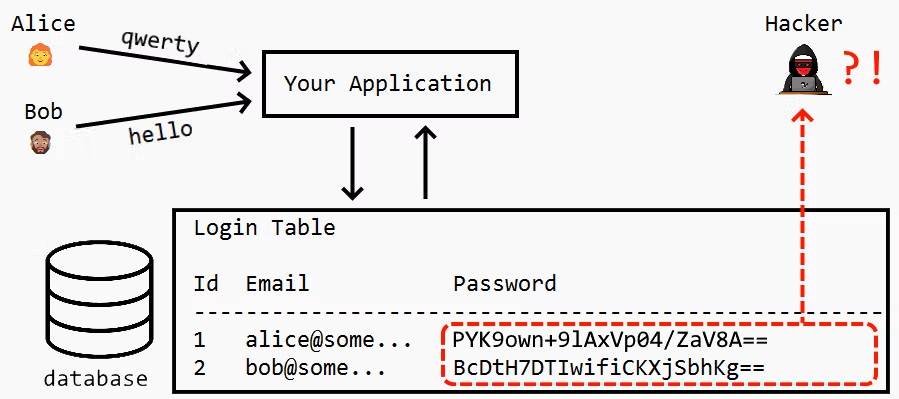
\includegraphics[width=0.6\textwidth]{obrazky-figures/be5db59264e538141840c7cbc012f8e5a8b94df7-899x399.jpg}
\caption{A visualization of the standard way to store passwords in a database (as described in an article by the Stytch Team \cite{what_is_password_hashing}) demonstrating how an unauthorized party cannot view the plaintext passwords directly from a leaked database.}
\end{figure}

\subsection{Cryptographic Primitives and the Speed-Security Paradox}
\label{speed-sec-paradox}

Historically, the selection of hashing algorithms for password storage was driven by the requirements of data integrity verification and digital signatures. Algorithms such as MD5 (Message Digest 5) and SHA-1 (Secure Hash Algorithm 1), as described by \cite{password_storage} and \cite{what_is_password_hashing}, were engineered for speed and efficiency on general-purpose Central Processing Units (CPUs). They rely heavily on bitwise operations—logical AND, OR, XOR, and bit rotations—that are computationally inexpensive and execute rapidly.

However, this design philosophy, while suitable for calculating file checksums or verifying SSL certificates, proved poorly suited to password storage. The efficiency that allows a system to verify a file's integrity in milliseconds also enables an attacker to compute billions of password candidates per second. When modern Graphics Processing Units (GPUs) are leveraged, with their thousands of Arithmetic Logic Units (ALUs) capable of high parallel instruction execution, algorithms like MD5 can be cracked at rates exceeding hundreds of gigahashes per second (GH/s). This phenomenon creates a "speed-security paradox": the faster a hash function is for the legitimate user, the more vulnerable it is to offline brute-force attacks.

To counter this, the cryptographic community moved toward specialized Password Hashing Schemes (PHS) and Key Derivation Functions (KDFs). These algorithms, including PBKDF2 (Password-Based Key Derivation Function 2), bcrypt, scrypt, and Argon2, introduce a tunable "work factor" or "cost" parameter. This parameter forces the hashing process to iterate purely computational work—such as performing the SHA-256 hash function 100,000 times recursively—to generate a single final digest. For a legitimate user attempting to log in, a 500-millisecond delay is imperceptible. For an attacker, this delay is multiplied by the size of the keyspace, rendering exhaustive search attacks computationally infeasible on a single machine.

\subsection{Salting and the Defense Against Precomputation}

A notable vulnerability in early password storage implementations was the storage of unsalted hashes. In such a system, identical passwords produce identical hashes. As described by \cite{what_is_password_hashing}, this deterministic property allows attackers to utilize Time-Memory Trade-off attacks, most notably employing Rainbow Tables \cite{enwiki:1333530676}, which are vast databases of precomputed hash chains that enable attackers to reverse a hash in constant time $O(1)$ by looking it up in the table rather than recomputing it. This trades storage space for computational time.

The defense against this is the "salt"—a random string of data generated using a cryptographically secure pseudorandom number generator (CSPRNG) that is concatenated with the user's password before hashing:

\begin{equation}
H_{stored}=Hash(P+S)
\end{equation}

The salt is stored in plaintext alongside the hash in the database. Its function is to ensure uniqueness. Even if two users choose the password "password123", their respective salts ($S_1$ and $S_2$) will differ, resulting in distinct stored hashes ($H_1$ and $H_2$). This neutralizes Rainbow Table attacks because the precomputed tables would need to be generated for every possible salt value, which is spatially impossible. However, according to \cite{complete_guide_passwd_hash}, salting does not stop dictionary or brute-force attacks; it merely forces the attacker to crack each hash individually rather than process them against a precomputed dataset.

\subsection{Memory-Hardness and Modern Algorithms}

As GPU acceleration became the standard for password recovery (a trend solidified by tools like Hashcat), hashing algorithms evolved to target the specific architectural weaknesses of GPUs. While GPUs possess immense computational throughput, they typically have limited high-speed memory available per core compared to a CPU. These modern algorithms are described by \cite{phs_explained}, \cite{complete_guide_passwd_hash}, \cite{app13169295} as follows:

\begin{itemize}
    \item \textbf{Bcrypt}: Based on the round-based Blowfish cipher, bcrypt utilizes a 4 KB state table that is constantly modified during the hashing process. This memory requirement limits the parallelism of GPUs, as the memory access pattern is data-dependent and unpredictable, forcing threads to stall while waiting for memory fetches.

    \begin{figure}[H]
    \centering
    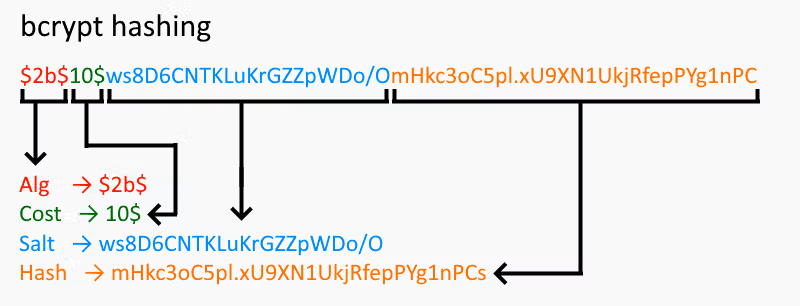
\includegraphics[width=0.7\textwidth]{obrazky-figures/7d29d3f05ffe6fe54105b51788cbed59f5bb4640-800x306.png}
    \end{figure}

    \begin{figure}[H]
    \centering
    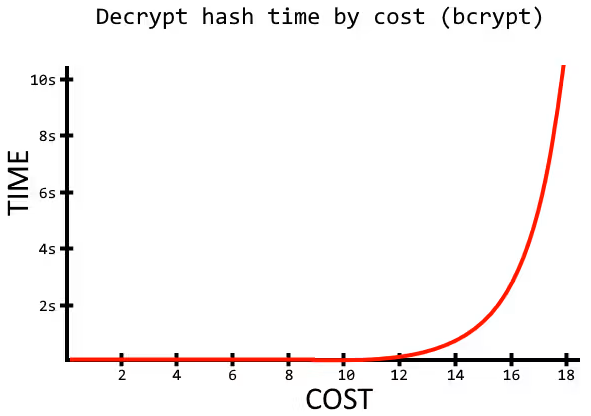
\includegraphics[width=0.7\textwidth]{obrazky-figures/7607b5515e4d19c9e2d48f3794e761ca78a3e852-730x471.png}
    \caption{Visualizations provided by \cite{what_is_password_hashing} depicting the adaptive bcrypt algorithm structure containing the used underlying algorithm (Blowfish), the rounds cost (which has a default value of 10 and scales exponentially with larger values, making the computation increasingly difficult), the randomly generated salt and the hash itself.}
    \end{figure}
    
    \item \textbf{Scrypt}: This algorithm was explicitly designed to be "memory-hard." It requires the generation of a large vector of pseudorandom data in RAM, which is then accessed in a random order to produce the final key. An attacker attempting to implement scrypt on a GPU or a custom ASIC (Application-Specific Integrated Circuit) must dedicate silicon area or VRAM to memory storage, reducing the number of parallel cracking engines that can fit on a single chip.

    \begin{figure}[H]
    \centering
    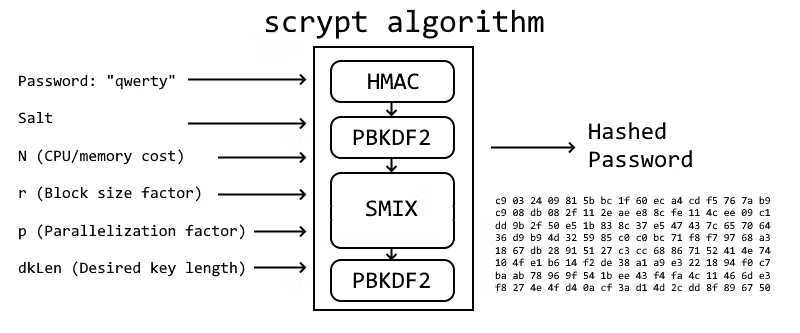
\includegraphics[width=0.8\textwidth]{obrazky-figures/99e4a2b570f1e127ac7dc33232ef3c8b807fb662-800x333.png}
    \caption{The Scrypt algorithm uses several steps to generate the final hash as described and visualised by \cite{what_is_password_hashing}. First, generating an expensive salt using the block size factor (the r parameter in Nrp) to create “blocks.” Next, using PBKDF2 to generate a large array whose size depends on the block size factor (r) and parallelization (p). The cost factor (N) is used as the number of times that each block is mixed using a function called ROMix. Scrypt then generates a new expensive salt by concatenating all mixed blocks. Finally, PBKDF2 uses the password and the calculated salt, trimming the output to the desired number of bytes (dkLen).}
    \end{figure}

    \item \textbf{Argon2}: Selected as the winner of the Password Hashing Competition in 2015, Argon2 offers three variants: Argon2d (data-dependent addressing, resistant to GPU cracking but vulnerable to side-channel attacks), Argon2i (data-independent addressing, resistant to side-channel attacks but slightly less resistant to TMTO), and Argon2id (a hybrid). Argon2 allows administrators to tune not only the time cost but also the memory cost and the degree of parallelism. This tri-parameter tuning allows defenders to optimize the hash for their specific server hardware while maximizing the cost for an attacker.
\end{itemize}



\section{Brute Force Attack}

The Brute Force attack, as described by \cite{enwiki:1323935452}, also known as an exhaustive key search or a mask attack in Hashcat, is the most theoretically sound method of password recovery. It relies on the mathematical certainty that if a password exists within a defined character set and length, systematically trying every possible combination will eventually yield the correct result. While often dismissed in casual discourse as inefficient, it serves as the baseline against which the strength of all encryption is measured and is the primary method for cracking complex, non-dictionary passwords.

\subsection{Keyspace Theory and Combinatorics}

The fundamental concept governing brute force attacks is the "keyspace"—the set of all possible permutations for a given password policy, as described by \cite{brute_force_math}. The size of the keyspace ($C$) determines the theoretical maximum time required to crack a password and is derived from combinatorial principles. The formula for the keyspace of a password of a fixed length $L$ using a character set of size $N$ is:

\begin{equation}
    C=N^L
\end{equation}

For a password policy that allows variable lengths (e.g., from 1 to 8 characters), the total keyspace is the summation of the permutations for each length increment:

\begin{equation}
    C_{total}=\sum_{i=1}^L N^i=N^1+N^2+...+N^L
\end{equation}

This exponential relationship means that linear increases in password length result in polynomial increases in attack difficulty. For instance, moving from a 7-character password to an 8-character password multiplies the keyspace by $N$. If $N=95$ (the full printable ASCII set), the 8-character password is 95 times harder to crack than the 7-character one. Conversely, increasing the character set size ($N$) generally yields diminishing returns compared to increasing length ($L$).

\subsection{Mask Attack Implementation in Hashcat}

In practical application within the Hashcat engine \cite{hashcat_wiki}, brute force is rarely executed as a blind iteration over an undefined range. It is instead implemented as a \textbf{Mask Attack} (Attack Mode 3) \footnote{https://hashcat.net/wiki/doku.php?id=mask\_attack}. A mask allows the attacker to define the structure of the candidates to be generated, optimizing the attack by eliminating structurally impossible candidates.

Hashcat utilizes a specific syntax to represent character sets within a mask:

\begin{itemize}
    \item \verb|?l|: Lowercase letters (a-z)

    \item \verb|?u|: Uppercase letters (A-Z)

    \item \verb|?d|: Digits (0-9)

    \item \verb|?h|: Hexadecimal lowercase (0-9, a-f)

    \item \verb|?H|: Hexadecimal uppercase (0-9, A-F)

    \item \verb|?s|: Special symbols

    \item \verb|?a|: All printable characters (?l +?u +?d +?s)

    \item \verb|?b|: All binary attributes (0x00 - 0xff)
\end{itemize}

A mask is constructed by concatenating these placeholders. For example, if an analyst knows a password consists of the prefix "Admin" followed by four digits, the mask would be: \verb|Admin?d?d?d?d|

This reduces the search from a full 9-character brute force (which would take centuries) to a 4-digit search ($10^4 = 10,000$ combinations), which Hashcat can resolve basically instantly.

\textbf{Custom Character Sets}: Hashcat allows for even greater granularity through custom character sets, defined using the flags \verb|-1|, \verb|-2|, \verb|-3|, and \verb|-4|. If, for example, a password policy requires "at least one uppercase letter and one digit," but the attacker wants to try a specific subset of symbols, they can define a custom set with the following command: \verb|hashcat -a 3 -1?d?s ?u?l?l?l?l?1|, where the custom set \verb|-1| is defined as digits plus symbols (\verb|?d?s|). The mask tries an uppercase letter (\verb|?u|), followed by four lowercase letters (\verb|?l|), followed by a character from the custom set (\verb|?1|). This precise targeting prevents the engine from wasting cycles on candidates that do not fit the known criteria.

\textbf{Increment Mode}: A standard mask attack (for example, \verb|?a?a?a?a?a?a?a?a|) only attempts passwords of exactly that length (8 characters). It does not check 7-character or 6-character passwords. To address this, Hashcat utilizes increment mode (\verb|--increment|), which automatically iterates the mask from a starting length (\verb|--increment-min|) to the full mask length (\verb|--increment-max|). This ensures that the entire keyspace of password candidates of varying lengths is covered up to the limit .

Furthermore, pure brute force assumes that all characters are equally likely in all positions. Human language behavior contradicts this, as each letter of the alphabet typically appears with different frequencies in common words. Hashcat supports \textbf{Markov Chain attacks}, which utilize a statistical model (defined in a .hcstat file) derived from large datasets of leaked passwords. This model predicts the probability of a character based on the preceding characters. By ordering the brute force generation based on these probabilities, Hashcat attempts the most "human-like" random strings first, statistically reducing the Time-To-Crack (TTC) for non-random passwords generated by humans. This mode is turned on by the Hashcat mask attack by default and uses a .hcstat file generated from the known rockyou.txt\footnote{https://hashcat.net/forum/thread-1710.html} wordlist. This mode can be turned off by launching Hashcat with the \verb|--markov-disable| CLI option.



\section{Dictionary Attack}

While brute force is mathematically comprehensive, the exponential growth of the keyspace renders it impractical for long passwords. The dictionary attack (Mode 0) exploits the linguistic nature of human-generated passwords, as described by \cite{enwiki:1320882747}. Users typically select passwords based on mnemonics, dictionary words, names, or cultural references to aid memorization. A dictionary attack iterates through a finite list of these candidates (a "wordlist") and hashes each one to compare against the target.

The efficiency of a dictionary attack is not primarily determined by the speed of the hardware but by the quality and relevance of the wordlist. A word list containing millions of English words will fail against a password like "P@ssw0rd!" as the exact string is not in the dictionary. To bridge this gap, modern cracking engines employ sophisticated rule-based permutations.


\subsection{Rule-Based Attack}

The \textbf{Rule-Based Attack} (utilized within Mode 0) \footnote{https://hashcat.net/wiki/doku.php?id=rule\_based\_attack} is one of Hashcat's most important practical capabilities because it transforms a static dictionary into a high-volume candidate generator \cite{hashcat_wiki}. Instead of requiring explicit storage of every candidate variant, rules act as a compact domain-specific language over each base word. For each input token, Hashcat executes one or more rule functions (e.g., case changes, positional edits, appends, prepends, substitutions), creating a large virtual candidate space at runtime.

From a performance perspective, this design is critical. The Hashcat documentation explicitly notes that regular-expression-style processing is too slow for the throughput needed to keep modern GPU kernels saturated; rule syntax is intentionally compact and execution-oriented to minimize candidate-generation overhead.

\textbf{Compatibility with John the Ripper}: Hashcat's rule engine is functionally compatible with John the Ripper (JtR) and PasswordsPro regarding shared function names, but the accepted argument sets can differ, so complex rule files are not always directly portable without adjustments.

\begin{table}[H]
\centering
\caption{Condensed overview of important Hashcat rule function groups.}
\label{tab:hashcat_rule_groups}
\small
\begin{tabular}{|p{3.0cm}|p{5.2cm}|p{5.2cm}|}
\hline
\textbf{Category} & \textbf{Representative functions} & \textbf{Typical purpose} \\\hline
Core transforms (JtR-compatible) & \verb|l|, \verb|u|, \verb|c|, \verb|t|, \verb|r|, \verb|d|, \verb|$X|, \verb|^X|, \verb|sXY|, \verb|@X| & Model common user edits: case patterns, reversing, duplication, suffix/prefix additions, leetspeak substitutions, and character removal. \\\hline
Positional edits & \verb|DN|, \verb|iNX|, \verb|oNX|, \verb|'N|, \verb|xNM|, \verb|ONM| & Target structural patterns at specific indexes, such as deleting, inserting, overwriting, truncating, extracting, and omitting character ranges. \\\hline
Hashcat-specific extensions & \verb|k|, \verb|K|, \verb|*NM|, \verb|+N|, \verb|-N|, \verb|LN|, \verb|RN|, \verb|yN|, \verb|YN| & Add non-JtR transformations such as swap-front/back, arbitrary index swaps, bitwise character shifts, ASCII increments/decrements, and block duplication. \\\hline
Memory-assisted rules & \verb|M|, \verb|XNMI|, \verb|4|, \verb|6| & Save intermediate states and re-insert substrings or full memorized words to generate compound candidates. \\\hline
Reject and condition rules & \verb|<N|, \verb|>N|, \verb|_N|, \verb|!X|, \verb|/X|, \verb|=NX|, \verb|\%NX| & Filter candidates by length/content constraints before expensive hash computation. In modern hashcat, reject rules have usage limitations (not regular rule-file behavior in all contexts) as documented in the wiki. \\\hline
\end{tabular}
\normalsize
\end{table}

\newpage
\begin{comment}
    
\textbf{Important rule-engine features}:

\begin{itemize}
    \item \textbf{Hex bytes in rules}: Hashcat supports \verb|\xNN| in rule definitions, enabling the insertion of non-printable bytes and exact byte-level transformations.

    \item \textbf{Multi-rules}: Multiple \verb|-r| arguments are combined combinatorially (Cartesian composition of rule lines) rather than executed as a simple sequential list of files. This expands coverage rapidly but can increase memory pressure.

    \item \textbf{Character class commands}: Since hashcat 7.0.0, commands prefixed with \verb|~| support class-aware operations (for a limited class set such as \verb|?l|, \verb|?u|, \verb|?d|, \verb|?h|, \verb|?H|, \verb|?s|). Some are supported on CPU and GPU, while some reject-oriented variants are CPU-only.

    \item \textbf{Rule debugging}: Using \verb|--stdout| allows for the inspection of generated candidates without running a full crack session, which is useful for both development and standalone candidate generation pipelines.

    \item \textbf{Matched-rule collection}: \verb|--debug-mode=1 --debug-file=<file>| stores rules that produced successful matches, enabling iterative optimization of rule sets.

    \item \textbf{Line complexity limits}: The wiki documents an upper bound on functions per rule line and across multi-rule composition, requiring careful design of complex chains.
\end{itemize}

\textbf{Random rule generation} is a Hashcat-specific exploration capability. Instead of relying only on predefined rule files, the engine can generate random rule sets at runtime:

\begin{itemize}
    \item \verb|--generate-rules=NUM| sets how many random rules are applied per base word.
    \item \verb|--generate-rules-func-min=NUM| and \verb|--generate-rules-func-max=NUM| bound the number of functions per generated rule.
    \item \verb|--generate-rules-func-sel=<list>| constrains the function pool (for example, \verb|ioTlc|).
\end{itemize}

This mechanism is useful when standard rule packs are exhausted and additional heuristic exploration is needed. In practical campaigns, it is most effective when paired with strict bounds on function count and a curated function-selection set to avoid uncontrolled candidate explosion.
\end{comment}



\subsection{Combinator Attack}

Passphrases consisting of multiple words are becoming increasingly common due to length-based security recommendations and ease of remembrance for end users, resulting in long passwords that are infeasible to crack by a brute force attack. Standard dictionary attacks also fail here because the space is included, or the combination is not a single token. The \textbf{Combinator Attack} (Mode 1) \footnote{https://hashcat.net/wiki/doku.php?id=combinator\_attack} addresses this by taking two dictionaries (or the same dictionary twice) and computing the Cartesian product of the two lists \cite{hashcat_wiki}.

\begin{equation}
    Candidate = Word_{Left} + Word_{Right}
\end{equation}

If dict1.txt contains "pass" and dict2.txt contains "word," the combinator attack generates "password". This mode is particularly effective when combined with rules that add separators, numbers, and other special symbols.

\subsection{Hybrid Attack}

The principle of hybrid attacks (Modes 6 and 7) \footnote{https://hashcat.net/wiki/doku.php?id=hybrid\_attack} is similar to the combinator attack, as it fuses the strengths of both dictionary and brute force attacks. They are designed to crack passwords that consist of a linguistic base followed or preceded by a random or patterned suffix/prefix \cite{hashcat_wiki}.

\begin{itemize}
    \item \textbf{Mode 6 (Wordlist + Mask)}: The engine takes a word from the dictionary and appends a brute-force mask to it.
    
 (Example command: \verb|hashcat -a 6 -m 0 <$hash> rockyou.txt ?d?d?d|)

    \item \textbf{Mode 7 (Mask + Wordlist)}: The engine prepends a mask to the dictionary word.
    
 (Example command: \verb|hashcat -a 7 -m 0 <$hash> ?d?d?d rockyou.txt|)
\end{itemize}


\subsection{Association Attack}

The \textbf{Association Attack} (Mode 9) \footnote{https://hashcat.net/wiki/doku.php?id=association\_attack} is a targeted mode designed for situations in which each hash has a corresponding per-account hint candidate (for instance, a username-derived token) \cite{hashcat_wiki}. Unlike a standard straight attack that tests all dictionary words against all hashes, association mode maps candidate lines to hash lines by index and tests them as associated pairs.

If we denote the hash list as $H=\{h_1,h_2,\dots,h_n\}$ and the associated candidate list as $W=\{w_1,w_2,\dots,w_n\}$, then mode 9 evaluates per-line associations of the form:

\begin{equation}
    h_i \stackrel{?}{=} Hash(R(w_i))\quad\text{for }i\in\{1,\dots,n\}
\end{equation}

where $R(\cdot)$ denotes an optional rule transformation pipeline.

According to the Hashcat wiki, two operational constraints are fundamental:

\begin{itemize}
    \item The wordlist must have exactly the same number of lines as the hash list.
    \item For hash types with work factor parameters (for example, bcrypt cost), all target hashes must use identical work factors.
\end{itemize}

\begin{comment}
This mode is especially useful as a high-value pre-pass for large salted datasets. Instead of spending resources on broad cross-product matching immediately, the attacker first evaluates context-linked candidates that are statistically more likely. Any recovered hashes are removed from later broader campaigns, reducing the remaining workload for regular straight, combinator, hybrid, or mask phases.

From an implementation perspective, association mode still supports rule processing. Therefore, a practical strategy is to run mode 9 with carefully chosen rule sets first, then continue with wider search modes. The wiki also notes that directories of wordlists can be used, but line-by-line alignment requirements must still be preserved for valid association semantics.
\end{comment}


\section{The Hashcat Engine}

Hashcat's dominance as the industry standard for password recovery is derived from its sophisticated internal engine, which is engineered to maximize the throughput of heterogeneous computing platforms. As described by \cite{bitwarden_hashcat}, Hashcat is designed from the ground up to exploit the Single Instruction, Multiple Data (SIMD) architecture of modern GPU accelerators using OpenCL, unlike legacy CPU-based crackers.

\subsection{Performance Tuning and Workload Profiles}

The throughput of the Hashcat engine is not static; it depends on how effectively the GPU pipeline is saturated. A GPU is a latency-hiding machine; it requires a large queue of work to keep all ALU cores busy while waiting for memory fetches. Hashcat provides granular control over this workload via several tuning parameters, as described in detail by the Hashcat documentation \cite{workload_profiles}.

\textbf{Workload Profiles} (\verb|-w|): This high-level parameter controls the size of the task batch sent to the GPU.

\begin{itemize}
    \item \verb|-w 1| (Low): Prioritizes low latency. Batches are small, meaning the GPU finishes quickly and returns control to the OS display driver. This keeps the desktop responsive but reduces cracking speed due to the overhead of frequent kernel launches.

    \item \verb|-w 2| (Default): A balance between responsiveness and performance.

    \item \verb|-w 3| (High): Prioritizes throughput. Large batches are queued. The desktop interface will likely freeze or lag significantly as the GPU is fully occupied with compute tasks.

    \item \verb|-w 4| (Nightmare): Maximizes batch size to the limits of the hardware. Designed for headless servers. This can cause the OS watchdog (TDR) to reset the driver if the batch takes too long to execute.
\end{itemize}

\subsection{Workload Distribution}

To tackle large keyspaces or to distribute work across a cluster of machines, Hashcat implements a deterministic keyspace segmentation strategy, as described by the Hashcat Wiki \cite{hashcat_wiki}. The basic terms to move forward are \footnote{https://hashcat.net/wiki/doku.php?id=distributing-work}:

\begin{itemize}
    \item \textbf{Keyspace}: Hashcat calculates the total work unit count for a given attack. This is accessible via the \verb|--keyspace| and \verb|--total-candidates| flags.

    \item \textbf{Segmentation}: The keyspace is a linear sequence of values. By assigning a specific offset (\verb|--skip|) and a chunk size (\verb|--limit|), the user can instruct Hashcat to process a specific slice of the keyspace.
\end{itemize}

This functionality is useful when designing a distributed system with Coordinator and Agent nodes working together to crack a given password hash with a large number of candidates. The exact strategy for using these parameters is described in later chapters.

\begin{figure}[H]
\centering
\includesvg[width=0.85\textwidth]{obrazky-figures/keyspace_segmentation.svg}
\caption{A conceptual visualization of keyspace segmentation in Hashcat. The total mathematically generated keyspace is treated as a linear array. By providing the skip parameter to set the starting index and the limit parameter to define the chunk size, an orchestrator can divide the work into non-overlapping segments for multiple Agents.}
\label{fig:keyspace_segmentation}
\end{figure}


\chapter{Distributed Computation Using the Actor Model}

This chapter examines the main theoretical and practical challenges of distributed computation and the architectural patterns used to address them. It focuses on the Actor Model as a paradigm for managing concurrency and state, and concludes with a comparison of three prominent .NET frameworks—Akka.NET, Microsoft Orleans, and Proto.Actor—to identify the most suitable foundation for a distributed cracking orchestrator.

\section{Challenges in Distributed Systems}

The distributed environment introduces several practical challenges, as summarized by the "Fallacies of Distributed Computing" chapter in \cite{distribution_challenges}, as a set of assertions that architects often incorrectly assume to be true: that the network is reliable, latency is zero, and bandwidth is infinite. In the specific domain of distributed password cracking, these fallacies manifest as tangible impediments to throughput (hashes per second) and correctness (keyspace coverage).

\subsection{Network Latency and Communication Overhead}
\label{net_lat_comm_ov}

Network latency—the time delay between the initiation of a network transmission and the receipt of the first unit of data, as described by \cite{distribution_challenges} and \cite{network_latency}—plays a pivotal role in the efficiency of a distributed cracker. This latency is distinct from bandwidth; while bandwidth measures the capacity of the pipe, latency measures the speed of travel through it. In a distributed environment, latency is composed of transmission latency, propagation latency, and processing delays at routers and switches.

In the context of password cracking, the impact of latency is non-uniform and depends on the cryptographic function being attacked. This relationship dictates the architectural requirements for the "Coordinator" or "Work Generator"—the component responsible for carving the keyspace into assignable chunks.

\textbf{The Latency-Throughput Correlation}: The notable metric in distributed cracking is the ratio of computation time to communication time, as described by \cite{distribution_challenges} and \cite{what_is_password_hashing}.

\begin{itemize}
    \item \textbf{Scenario A: Slow Hashes (High Computational Cost)}: When attacking algorithms like bcrypt with high iteration counts, a single candidate password may require milliseconds of GPU time. A relatively small batch of candidates can occupy a worker node for minutes. In this scenario, network latency is negligible. Even if the round-trip time (RTT) for requesting a new job is 500 ms, it represents a fraction of a percent of the total job execution time. The system is "compute-bound."

    \item \textbf{Scenario B: Fast Hashes (Low Computational Cost)}: Conversely, algorithms like NTLM or MD5 allow modern GPUs to compute billions of hashes per second. If the orchestrator assigns a small keyspace segment (e.g., 100 million candidates), a high-end GPU might exhaust this workload in milliseconds. If the network latency to request the next batch is 50 ms, the GPU spends more time idling (waiting for work) than computing. This phenomenon can cause node starvation, degrade the aggregate cluster performance, and make the system "network-bound".
\end{itemize}

\textbf{Bandwidth Constraints}: While latency impacts the control plane, bandwidth constrains the data plane. Distributed cracking often involves the dissemination of large dictionaries (wordlists) or rule files. The fallacy that "bandwidth is infinite" leads to bottlenecks when an orchestrator attempts to simultaneously push a multi-gigabyte wordlist to hundreds of worker nodes. Architectural mitigations must include local caching strategies, compression, or the use of peer-to-peer distribution protocols (like BitTorrent) to alleviate strain on the central server. Furthermore, the variability of network performance—caused by congestion, packet loss, and jitter—means that no finite protocol can guarantee deterministic delivery times. The system must be designed to tolerate unbounded latency, never assuming that a delayed response implies a failed node.

\subsection{Partial Failures and System State}
\label{part_fails_sys_state}

The defining characteristic of a distributed system is the concept of partial failure. In a monolithic application, components share a fate; if the memory bus fails, the entire application halts. As depicted by \cite{distribution_challenges} and \cite{distribution_challenges_amazon}, in a distributed cluster, one component (e.g., a worker node) may fail while others (e.g., the server or database) continue to operate correctly. This creates a state of deep uncertainty.

\textbf{The Three-State Nature of Remote Operations}: When an orchestrator sends a command to a worker node, the outcome is not binary (Success/Failure) but ternary:

\begin{enumerate}
    \item \textbf{Success}: The worker receives the command, executes it, and acknowledges completion.

    \item \textbf{Failure}: The worker receives the command but cannot execute it (e.g., the plaintext password was not found, or there was a GPU driver error) and reports a failure.

    \item \textbf{Unknown}: The orchestrator receives no response. The failure could be located in the request path (the worker never got the job), the execution phase (the worker is executing the job but is slow), or the response path (the work is done, but the acknowledgement was lost). If the orchestrator assumes the worker failed and re-assigns the job to another node, it risks duplicating work—an inefficiency that, while tolerable, wastes resources. More critically, if the orchestrator assumes the worker succeeded (perhaps due to a timeout logic error) and marks the chunk as done, the system incurs data corruption: a segment of the keyspace has been skipped, and the password may be missed. This mandates the implementation of robust timeout and retry mechanisms, often utilizing "heartbeats" to distinguish between a slow node and a dead node. However, even heartbeats are imperfect; a node under heavy load may fail to respond to a heartbeat while still successfully processing a job.
\end{enumerate}

\section{Reliability Strategies}
%\begin{itemize}
%    \item \textbf{Checkpointing:} Saving progress states to allow resumption after crashes[cite: 24].
%    \item \textbf{Idempotency:} Ensuring that repeated task execution does not corrupt aggregated results.
%\end{itemize}

To engineer a system that remains robust in the face of the aforementioned challenges, two primary reliability strategies are employed: checkpointing and idempotency. These patterns allow the system to make forward progress despite interruptions and ensure data integrity despite message duplication.

\subsection{Checkpointing}

Checkpointing, as described in \cite{checkpointing}, is the technique of persisting the state of a running process so that, in the event of a failure, execution can resume from the last saved state rather than restarting from the origin. In distributed password cracking, this concept operates at two distinct levels: the granular task level (Distributed Checkpointing) and the engine level (Local Checkpointing).

\textbf{Local Checkpointing (Engine Level)}: The underlying cracking engine, Hashcat \cite{hashcat_wiki}, implements a native checkpointing mechanism. As it iterates through a specific mask or wordlist, it maintains a .restore file. This binary file records the precise position in the keyspace loop where the engine is currently operating. If the Hashcat process is terminated (e.g., via user interruption or power loss), relaunching the executable with the \verb|--restore| flag allows it to read this file and resume operations exactly where it left off. However, relying solely on local checkpointing is insufficient for a distributed cluster. The orchestrator would have no visibility into how much of the assigned work was actually completed \footnote{https://hashcat.net/wiki/doku.php?id=restore}.

\textbf{Distributed Checkpointing (Task Granularity)}: To survive the loss of individual nodes, the system must implement checkpointing at the orchestration level. This is achieved through \textbf{Keyspace Segmentation}.

\begin{enumerate}
    \item \textbf{Segmentation}: The global keyspace is divided into discrete, immutable "Work Units" or "Chunks" (for example, as a mechanism described in \cite{BUT168182}).

    \item \textbf{State Tracking}: The orchestrator maintains the status of each chunk in a persistent database (e.g., Pending, Running, Completed).

    \item \textbf{Checkpoint}: In this architecture, the successful completion and acknowledgement of a Work Unit is the checkpoint. The system does not attempt to save the precise state of every GPU register across the network in real-time. Instead, it relies on the atomicity of the Work Unit.
\end{enumerate}

If a node crashes while working on a chunk, the orchestrator detects the timeout and re-queues the entire chunk for another node. While this results in a small amount of duplicated work, it guarantees that no gaps are left in the keyspace. This approach aligns with "Uncoordinated Checkpointing" strategies, where global consistency is maintained by the independence of tasks rather than a global freeze-and-save protocol. To optimize this, the size of the Work Unit must be tuned: small enough that a retry is inexpensive but large enough to amortize the network latency overhead (as discussed in \ref{net_lat_comm_ov}).

\newpage

\subsection{Idempotency}

Idempotency, as depicted in \cite{idempotency}, is a property of an operation whereby applying it multiple times yields the same result as applying it once. In mathematical terms, a function $f$ is idempotent if $f(f(x)) = f(x)$. In distributed systems, this property is the primary defense against the "at-least-once" delivery semantics of unreliable networks.

\textbf{The Necessity of Idempotency}: Because network acknowledgements can be lost (as discussed in \ref{part_fails_sys_state}), an orchestrator must be aggressive in retrying tasks. If a worker completes a job but the "Completed" message is dropped, the orchestrator will eventually time out and re-send the job to a different worker. This leads to the same job being executed twice.

\begin{itemize}
    \item \textbf{Non-Idempotent System}: If the system simply counts "Total Hashes Checked" by adding the job size to a running total, processing the job twice results in an inflated, incorrect hashrate and progress percentage.

    \item \textbf{Idempotent System}: If the system marks a specific Job ID as "Completed," processing the completion message a second time changes nothing; the Job ID is already marked.
\end{itemize}

\textbf{Implementation Patterns}: To achieve idempotency in a cracking cluster, several patterns are essential:

\begin{itemize}
    \item \textbf{Idempotency Keys}: Every request and work unit must be assigned a deterministic Unique Identifier (UUID) at creation. This UUID serves as the idempotency key. When a worker reports a result, it includes this key. The database layer uses this key to enforce uniqueness, ensuring that duplicate reports do not create duplicate entries.

    \item \textbf{Upsert Logic}: Database operations should utilize "Upsert" (Update or Insert) semantics. For example, when updating a job status, the query should be
    
       \verb|"Set Status to 'Completed' WHERE JobID = X"|.
    
       Running this query multiple times has the exact same effect as running it once.

    \item \textbf{Result Deduplication}: In a scenario where multiple nodes might redundantly crack the same hash, the system must check whether the hash is already present in the "Cracked" table before inserting it.
\end{itemize}

By baking idempotency into the API and database schema, the system becomes resilient to network "stuttering," retries, and the chaotic replay of messages that often accompanies system recovery.

\newpage
\section{Core Concepts of the Actor Model}
\label{sec:core_actor_concepts}

To manage the high concurrency and state complexity of distributed cracking, the Actor Model, as described by \cite{enwiki:1323072662}, provides a suitable theoretical framework for this context compared with traditional object-oriented programming (OOP). Originating in 1973 with Carl Hewitt, the Actor Model treats "Actors" as the universal primitives of concurrent computation, offering a high-level abstraction that aligns well with distributed systems.

\subsection{State and Behavior}

In traditional concurrent programming (e.g., utilizing threads and locks), shared memory is the primary medium of interaction. This leads to complex race conditions and deadlocks. The Actor Model inverts this: \textbf{Actors share nothing} and only communicate by sending messages to each other's mailboxes, as described in \cite{actor_model_understanding}.

According to the fundamental principles of the Actor Model (as concisely summarized in \cite{proto_actors_docs}), an actor encapsulates its internal state, behavior, and mailbox into a single, isolated entity that is driven by external events.

\begin{figure}[H]
\centering
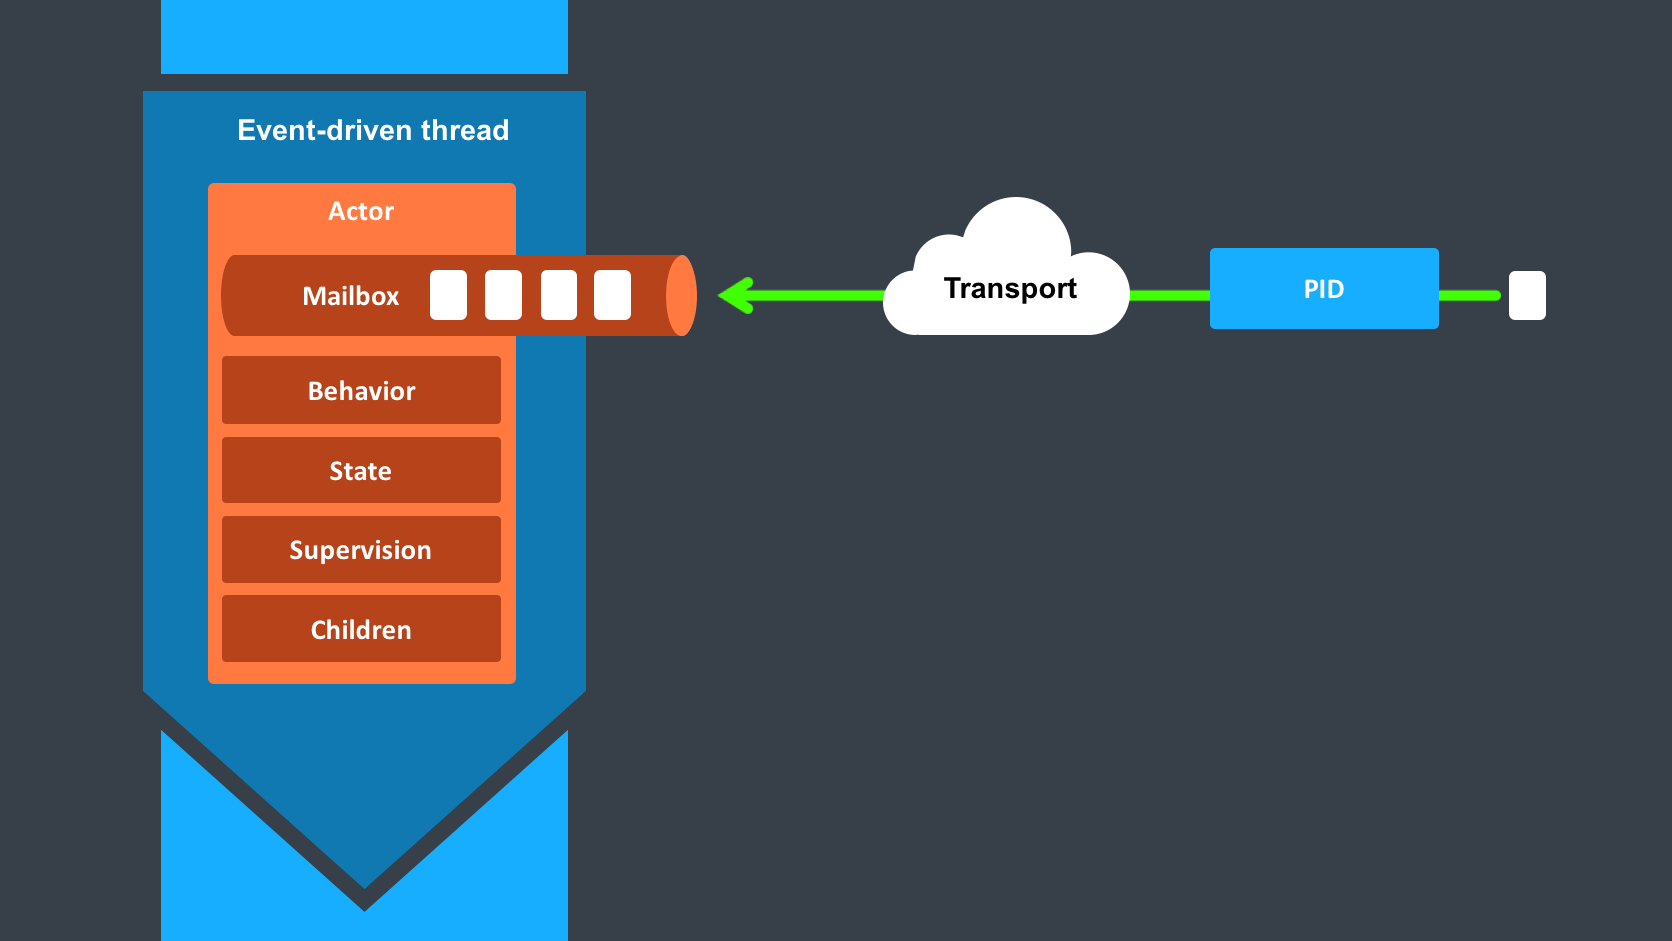
\includegraphics[width=1.0\textwidth]{obrazky-figures/actor-d79f93eee9d91cbce869f0a5944b26f5.png}
\caption{A conceptual visualization of an actor's internal anatomy adapted from \cite{proto_actors_docs}. The actor operates on an event-driven thread, connecting to the asynchronous network via its \textbf{Mailbox}. It encapsulates its private \textbf{State} (preventing external access) and uses its \textbf{Behavior} to process incoming messages sequentially. It can also manage a hierarchy of \textbf{Children} for localized fault tolerance.}
\label{fig:actor-thread}
\end{figure}

\subsection{Mailboxes, References, and Asynchronous Messaging}

Communication in the Actor Model is exclusively asynchronous. To send a message, the sender must possess a unique logical reference to the recipient's mailbox. This reference typically encapsulates both the physical network address of the host node and the unique string identifier of the specific actor instance. An actor routes a message to another actor's reference and immediately continues its own execution, avoiding blocking operations. This non-blocking nature is important for the scalability of the orchestration layer.

The mailbox is an important architectural component \cite{proto_mailboxes_docs}. When a message is sent to an actor, it is not executed immediately by the sender's thread; instead, it is safely enqueued. A dedicated dispatcher then polls this mailbox and invokes the actor's message-handling routine. Crucially, the dispatcher ensures that an actor processes \textbf{exactly one message at a time}. 

For a password cracking cluster, a job Coordinator actor holds the state of the keyspace. Because only the Coordinator can modify this state, and because its mailbox guarantees sequential message processing, race conditions are structurally prevented. Two worker nodes cannot simultaneously work on the same chunk because the Coordinator processes the first request entirely, updates its state, and only then dequeues the second request. This "single-threaded illusion" simplifies the mental model for developers and removes the need for complex thread-synchronization primitives such as mutexes or semaphores.

\subsection{The Actor Lifecycle}

Beyond simply processing application messages, actors possess a strictly managed lifecycle \cite{proto_lifecycle_docs} controlled by the underlying framework. The framework dispatches specific system messages to the actor to notify it of state transitions, allowing developers to execute precise initialization and cleanup logic without blocking the main execution path:

\begin{itemize}
    \item \textbf{Starting / Started}: Triggered immediately after the actor is instantiated but before it processes any external mail. This is utilized to safely establish database connections or initialize background telemetry timers.
    
    \item \textbf{Restarting}: Invoked when an actor is about to restart. Its object is destroyed, so this event allows the execution of some teardown logic to perform a graceful shutdown (e.g. persist a state to a database).

    \item \textbf{Stopping}: The actor has been instructed to terminate. It finishes processing the currently active message but rejects any new incoming messages. Similar to the restarting state, where a graceful shutdown should be handled.

    \item \textbf{Stopped}: The actor has stopped execution and is no longer able to send or receive messages from its mailbox. When this message is processed, the actor object is scheduled for garbage collection.
\end{itemize}

\subsection{Supervision Strategy: Hierarchical Fault Tolerance}

The Actor Model handles failure through a strict parental hierarchy, as described by \cite{actor_supervision}. When an actor is created, it is the child of the actor that created it. This establishes a supervision tree. The core philosophy, popularized by Erlang, is "Let It Crash." Instead of defensive programming (wrapping every line in \verb|try/catch|), actors are allowed to fail.

When a child fails, their parent intercepts the error and decides how to react using the following \textbf{Supervision Directives}: 

\begin{itemize}
    \item \textbf{Restart}: The error corrupted the state (e.g., an unhandled exception). The parent kills the child and starts a fresh instance. The internal state is wiped, but the "identity" (mailbox) remains, processing queued messages.
    
    \item \textbf{Stop}: The error is fatal, and the child is permanently terminated.
    
    \item \textbf{Escalate}: The parent does not know how to handle the error and fails, passing the problem up to the grandparent actor.
    
    \item \textbf{Resume}: The error is trivial (e.g., a corrupt log entry), and the child retains its state and processes the next message.
\end{itemize}

Whatever action is taken on a parent propagates to its children. If a parent is halted, all its children halt. If it is restarted, all its children restart.

Failure of a node may affect other actors in a cluster in two ways:

\begin{itemize}
    \item \textbf{One-For-One}: The directive applies only to the failing child. This is the standard for independent workers. For example, if GPU Node 1 crashes, the Supervisor restarts Node 1. Node 2 is unaffected.

    \item \textbf{All-For-One}: The directive applies to all children of the supervisor. This is used when actors are tightly coupled. For example, if a "File Reader" actor fails in a pipeline, the "File Parser" and "Database Writer" actors might also need to be restarted because they are now out of sync.
\end{itemize}

For a distributed cracker, the One-For-One strategy is essential to ensure that a single faulty node does not destabilize the entire cluster.



\section{Analysis of Actor Model Frameworks Available for .NET}

The .NET ecosystem has broadened its support for the Actor Model. There are three primary frameworks commonly used in this space: \textbf{Akka.NET}, \textbf{Microsoft Orleans}, and \textbf{Proto.Actor}. Each framework interprets the Actor Model differently, balancing performance, ease of use, and explicit control in different ways.

\subsection{Akka.NET}

Akka.NET is a port of the JVM-based Akka framework, widely considered the gold standard for Actor Model implementations in enterprise systems. It provides a comprehensive, developer-friendly ecosystem.

\textbf{Architecture and Features}:

\begin{itemize}
    \item \textbf{Explicit Actors}: Akka.NET requires developers to explicitly define actor classes, manage their creation (using the \verb|Props| class), and orchestrate the supervision hierarchy. This explicitness offers granular control over the system's behavior.

    \item \textbf{Clustering and Gossip}: The Akka.Cluster module \cite{akka_cluster} implements a decentralized membership protocol where nodes communicate via a Gossip Protocol, exchanging state information to converge on a view of the cluster members. This creates a peer-to-peer network with no single point of failure.

    \item \textbf{Persistence}: The Akka.Persistence module \cite{akka_persistance} supports Event Sourcing. Actors can persist their internal state changes as a sequence of events. If an actor crashes and is restarted (even on a different node), it replays these events to restore its state. This is ideal for a job Coordinator that must not lose track of assigned chunks.
\end{itemize}

\textbf{Performance}: Akka.NET uses the DotNetty transport layer (TCP/UDP). It includes self-optimizing batching systems that group messages to reduce network overhead. Benchmarks from \cite{akka_performance} indicate it can handle approximately 190,000 messages per second in batched scenarios on standard hardware. While high, this throughput is bounded by the overhead of the detailed actor context serialization.

\subsection{Microsoft Orleans}

Microsoft Orleans, created by Microsoft Research, introduces a radical evolution of the model described in \cite{orleans_overview}: the "Virtual Actor" or "Grain," which, unlike Akka's actors that must be explicitly created and started, are virtual entities that always exist logically. This approach has many quality of life benefits, as described by \cite{orleans_benefits}.

\begin{itemize}
    \item \textbf{Activation on Demand}: A Grain is automatically activated (instantiated in memory) by the runtime only when a message is sent to it. The developer does not manage the lifecycle.

    \item \textbf{Deactivation}: When a Grain is idle, the runtime deactivates it (removes it from memory) to free up resources.

    \item \textbf{Location Transparency}: The runtime handles the placement of Grains on silos (servers). A "Grain Directory" tracks where each Grain resides.
\end{itemize}

\textbf{Performance}: Orleans is optimized for high-concurrency, low-latency I/O-bound workloads (e.g., web requests). According to \cite{orleans_perf}, it employs a cooperative multitasking model where Grains execute on a limited number of threads (typically one per CPU core). This presents a significant challenge for password cracking. If a Grain executes a long-running CPU-bound task (like calculating a complex hash or managing a large batch of work), it blocks the thread. This "starves" the silo, preventing it from processing other messages, heartbeats, or acknowledgements. To work around this, developers use \verb|StatelessWorker| grains or explicitly offload work to the .NET ThreadPool (with \verb|Task.Run|), which breaks the single-threaded safety guarantees of the Grain model and introduces complexity.
While libraries like \textit{Orleans.SyncWork}\footnote{https://github.com/OrleansContrib/Orleans.SyncWork/tree/main} exist to mitigate this, the framework fights against the nature of heavy computational tasks.

\subsection{Proto.Actor}

Proto.Actor was created by Roger Alsing, a co-founder of Akka.NET, specifically to address perceived architectural limitations in Akka.NET regarding performance and complexity, as described by \cite{about_proto_actor}. It is a cross-platform framework (C\#, Go, Kotlin) built on Google's gRPC high-performance Remote Procedure Call (RPC) messaging framework.

\begin{itemize}
    \item \textbf{gRPC and Protobuf}: Proto.Actor leverages Protocol Buffers for serialization and gRPC streams for transport. This results in low overhead. Benchmarks have shown Proto.Actor capable of handling about 2.5 million messages per second over the network, significantly outperforming Akka.NET's \textasciitilde190k.

    \item \textbf{Hybrid Model}: Proto.Actor supports both "Classic Actors" (explicit lifecycle, like Akka) and "Grains" (virtual actors, like Orleans via the Proto.Cluster package \cite{about_proto_cluster}), giving developers flexibility to mix paradigms. Virtual Actors provide the location transparency needed for orchestration layers, while Classic Actors offer the explicit lifecycle control and direct process binding required for hardware-coupled edge compute nodes.

    \item \textbf{Precise Control via PIDs and Lifecycle Hooks}: Aligning with the theoretical concepts discussed in Section \ref{sec:core_actor_concepts}, Proto.Actor implements the unique actor reference as a \verb|PID| (Process Identifier) \cite{proto_actors_docs}. Furthermore, it exposes explicit framework-level messages—such as \verb|Started| and \verb|Stopped| \cite{proto_lifecycle_docs}—which are seamlessly integrated into the actor's standard message-handling behavior. This enables exact programmatic control over resource allocation, empowering the system to safely initialize background telemetry timers or gracefully halt Hashcat instances upon actor termination.

    \item \textbf{Pluggable Clustering}: Rather than implementing a monolithic clustering engine, Proto.Actor outsources cluster membership to dedicated providers like \textbf{Consul}, \textbf{Kubernetes}, or \textbf{etcd}. This allows it to leverage existing cloud-native infrastructure for reliability.
\end{itemize}



% =========================================
% CHAPTER 4: SYSTEM ANALYSIS AND ARCHITECTURE
% =========================================
\chapter{System Analysis and Architecture Design}
\label{chap:analysis}

This chapter provides an overview of requirements, analyzes existing solutions in the distributed password cracking space, and proposes an improved Actor-based design for a system based on the theoretical background contained in previous chapters.

\section{Requirements Analysis}

The development of a distributed password cracking system introduces a different set of constraints from those of a typical web service. The system must coordinate computationally intensive tasks across heterogeneous hardware while preserving strict synchronization of the keyspace so that no candidate passwords are skipped.

\subsection{Functional Requirements}

\begin{itemize}
    \item \textbf{Distributed Keyspace Management}: The system must be capable of calculating the total keyspace of a given attack and segmenting it into discrete, non-overlapping "Work Units" or "Chunks."

    \item \textbf{Heterogeneous Node Support}: The scheduling algorithm must accommodate nodes with vastly different performance profiles (e.g., a laptop with an integrated GPU vs. a server with multiple dedicated GPUs). Faster nodes must consume larger chunks of the keyspace to prevent starvation.

    \item \textbf{Attack Mode Support}: The system must support the core Hashcat attack modes (e.g., Mask, Dictionary with or without rules, Combinator, Hybrid, and Association Attack).

    \item \textbf{Job Control}: Administrators must have the ability to easily input attack parameters and start and abort jobs globally.

    \item \textbf{Result Aggregation}: Plaintext passwords recovered by any node must be securely transmitted to the Coordinator and stored immediately.
\end{itemize}

\subsection{Non-Functional Requirements}

\begin{itemize}
    \item \textbf{High Throughput Messaging}: The orchestration layer must handle high-frequency telemetry updates (hashrate, temperature, job progress, etc.) from hundreds of nodes without becoming a bottleneck. This requirement specifically drives the selection of \textbf{Proto.Actor} over Akka.NET or Microsoft Orleans, as Proto.Actor's gRPC-based transport layer demonstrates significantly lower serialization overhead and higher message throughput in high-concurrency scenarios.

    \item \textbf{Fault Tolerance}: The system must survive the sudden loss of any worker node without data corruption. Unfinished work units from failed nodes must be automatically reassigned.

    \item \textbf{Concurrent Data Access}: The backing storage must smoothly handle parallel operations. The distributed actor system will constantly bulk-insert progress updates and recovered passwords, while the web interface simultaneously queries this exact data to render live user dashboards.

    \item \textbf{Low Latency Overhead}: The time required to assign a new work unit must be negligible compared to the time required to process it. For fast hashing algorithms (e.g., NTLM or MD5), the amount of messages transferred over the network should be minimal, favoring larger chunks. This raises the need to design a dynamic chunking algorithm that sets the size of the work unit based on the Agent node's capabilities (the hash rate metric provided by Hashcat's \verb|--benchmark| flag can provide this insight).
\end{itemize}

\section{Analysis of Existing Solutions: FitCrack and Hashtopolis}

To contextualize the proposed architecture, it is useful to evaluate the two prominent open-source distributed cracking systems currently available: \textbf{FitCrack} and \textbf{Hashtopolis}. Both systems wrap the Hashcat engine but employ different architectural paradigms that influence their performance and suitability for specific use cases.

\subsection{FitCrack}

As described by its authors in \cite{BUT168182}, FitCrack is a distributed password cracking system built on top of the \textbf{BOINC} (Berkeley Open Infrastructure for Network Computing) framework. It was developed primarily for digital forensics and research at the Brno University of Technology.

The architecture of FitCrack utilizes a "Volunteer Computing" model. The server encapsulates cracking tasks into independent "Work Units" that are pushed to client queues. Clients download these units, process them offline, and upload the results upon completion.

Its arguable strength is high fault tolerance because it is designed for volunteer grids (like SETI@home); it assumes clients are unreliable. It handles node disconnections gracefully by automatically re-issuing uncompleted work units. However, it can suffer from high latency because BOINC is not designed for real-time responsiveness; canceling or modifying a job takes time to propagate.

For \textbf{Mask Attacks}, FitCrack divides the calculated keyspace into fixed-size chunks. Due to the high communication latency inherent in the BOINC protocol, these chunks must be sufficiently large (often requiring minutes or hours to compute) to avoid network bottlenecks. 

For \textbf{Dictionary Attacks}, FitCrack traditionally relies on physically distributing the wordlist files (or pre-sliced segments of them) to the client nodes. While robust, this approach imposes significant bandwidth costs and requires substantial local storage on the Agent machines, especially when utilizing large multi-gigabyte dictionaries.

\subsection{Hashtopolis}

Hashtopolis provides us with insights into a different approach in this field. As described in \cite{hashtopolis}, it is a client-server management platform widely adopted by the penetration testing community. It uses a PHP/MySQL backend and Python-based Agents.

Its architecture operates on a Pull-Based model via a REST API. Agents periodically poll the server (e.g., every 5-30 seconds) to request a "Chunk" of work.

One of its strengths is the comprehensive web interface provided for managing "Supertasks" (chained attack modes), uploading wordlists, and visualizing cluster heatmaps. Unlike FitCrack, it features granular control that allows for relatively fast job cancelation and modification. However, its reliance on HTTP polling creates significant network overhead as the cluster grows. Thousands of Agents polling a PHP server every few seconds can induce a Denial-of-Service (DoS) condition on the control plane. Additionally, the central MySQL database often becomes a point of contention for writing status updates and chunk assignments, limiting linear scalability.

In \textbf{Mask Attacks}, Hashtopolis attempts to mitigate hardware heterogeneity by dynamically sizing blocks of the keyspace based on an Agent's benchmarked speed. However, because it relies on a central relational database to calculate, assign, and track these non-overlapping chunks, issuing them to hundreds of polling Agents simultaneously can lead to database lock contention. This architectural bottleneck limits the platform's ability to scale linearly.

For \textbf{Dictionary Attacks}, Agents are required to download the necessary wordlists locally in advance or on-demand. It then orchestrates the attack by sending specific \verb|--skip| and \verb|--limit| line-number directives. While effective, parsing millions of newlines to reach a high \verb|--skip| value introduces a computational penalty on the Agent before hashing even begins.

\newpage

\section{Proposed Actor-Based Architecture}

The system architecture adopts a three-tier topology consisting of Manager, Coordinator, and Agent nodes, implemented using the \textbf{Proto.Actor} framework. The architectural design utilizes specific Proto.Actor features of Virtual Actors (Grains) and Classic Actors. This hybrid approach is not supported by either Akka.NET or Microsoft Orleans. Unlike FitCrack, which relies on the polling-based BOINC infrastructure or the REST API model used by Hashtopolis, this system utilizes a persistent gRPC connection maintained by the actor system, allowing for real-time bi-directional asynchronous communication. 

\subsection{The Coordinator Node}

The Coordinator service is split into two parts: \textbf{Manager} and \textbf{Coordinator} in the .NET solution as Virtual Actors / Grains that can be easily addressed by their names by connected Agent nodes in the cluster.

The Manager node serves as the root state manager, cluster leader, and web server. It does not orchestrate the active cracking Agents directly; instead, it handles the high-level lifecycle of jobs and data persistence.

\begin{comment}
\begin{itemize}
    \item \verb|JobManagerGrain|: The root supervisor Grain for all cracking operations. When a new job is submitted via the web UI, it registers the job in the database and spawns a dedicated Coordinator specifically for that task.
\end{itemize}
\end{comment}

Next, the job Coordinator node is a dedicated, headless orchestration node designed to relieve the Manager's web server of the heavy network I/O associated with handling thousands of Agent requests per second. It was designed to launch as a separate process so that the cluster can contain multiple Coordinator nodes to scale horizontally as the orchestration load grows.
    
\begin{comment}
\begin{itemize}
    \item \verb|JobCoordinatorGrain| (Virtual Actor / Grain): A unique actor assigned to a specific Job ID, hosted entirely on a Coordinator node. It holds the "Global Cursor" of the keyspace. It is responsible for generating work chunks and tracking their state (Pending, Assigned, or Completed). By implementing this as a Virtual Actor (Grain), we ensure that the job state is always addressable and effectively "single-threaded," naturally preventing race conditions where two workers might attempt to claim the exact same keyspace chunk. Furthermore, because Grains are location-transparent, the failure of a specific Coordinator host merely causes the cluster to instantly reactivate the Grain on another healthy server, ensuring high availability of the control plane without manual intervention.

    \item \verb|ResultCollectorGrain|: A specialized actor that receives successful "Cracked" messages from the cluster. It interfaces directly with Entity Framework Core to map and store the recovered passwords into the PostgreSQL database and notifies the relevant \verb|JobCoordinatorGrain| to halt further work if a target hash has been fully compromised.
\end{itemize}
\end{comment}

\subsection{The Agent Node}

The Agent runs as a standalone, lightweight .NET console application on the compute nodes. Its primary responsibility is to launch a local Hashcat process to keep the underlying GPU hardware saturated with hashing instructions and report back to the Coordinator node with the result of its assigned work.

\begin{comment}
\begin{itemize}
    \item \verb|AgentService|: The top-level supervisor on the client machine. It manages the connection to the cluster and supervises the worker actors.

    \item \verb|WorkerActor| (Classic Actor): Implements the "Work Pulling" pattern. Unlike the Coordinator, the Agent relies on Proto.Actor's "Classic" Actors rather than Virtual Grains. Because a compute node is fundamentally tied to its physical hardware resources (the GPU), location transparency is not desired. If a machine loses power, the system should not automatically spawn its \verb|WorkerActor| on another node, as the specific hardware context cannot be migrated. Its unique identity within the cluster is directly derived from its Proto.Actor \verb|PID| (Process Identifier, consisting of the node's IP address and a unique ID string). This allows the Coordinator to unambiguously route messages back to the exact physical machine that requested them. When the current task is near completion, it preemptively sends a \verb|RequestWork| message to the \verb|JobCoordinatorGrain| to fetch the next chunk, ensuring zero downtime between batches.

    \item \verb|HashcatWrapper|: An encapsulated service that manages the OS-level Hashcat process. It translates actor messages into executable arguments (e.g., converting a given chunk range into \verb|--skip| and \verb|--limit| flags) and parses the standard output streams from Hashcat to continuously report progress and hardware telemetry back to the \verb|NodeGuardian|.
\end{itemize}
\end{comment}

\section{Communication Protocol}

The system's interactions are formally defined using \textbf{Protobuf} (Protocol Buffers) \verb|service| and \verb|message| definitions \cite{about_proto_cluster} for all wire serialization, which is native to Proto.Actor. This provides a strictly typed, compact binary format that is significantly faster than JSON or XML used in standard REST API based systems.

To bridge the gap between these language-agnostic contracts and the C\# application, the architecture employs the \verb|Proto.Cluster.CodeGen| library \cite{proto_codegen}. During compilation, this toolchain parses the \verb|.proto| files and automatically generates the required C\# boilerplate. This includes the strongly typed message classes, the client interfaces used to transparently call the actors across the network, and the abstract base classes (e.g., \verb|JobCoordinatorGrainBase|) from which the concrete Grain implementations inherit. This strictly enforces the API contract at compile-time, prevents data structure drift between the Manager and Agent nodes, and cleanly maps the conceptual design to Proto.Actor Virtual Grains.

\subsection{Message Flow: The Work Pulling Pattern}

Instead of the Coordinator "pushing" pre-planned static Work Units (which risks overwhelming slow nodes), the Workers "pull" dynamically sized Work Units based on their hardware capabilities. The cracking process is initiated by the Agent nodes in the following way:

\begin{enumerate}
    \item \textbf{Job Discovery}: If the Agent has just joined the cluster or if its previous job is finished or canceled, it invokes the \verb|JobDiscovery| RPC on the root \verb|JobManagerGrain|, passing its unique \verb|AgentId|. The Manager responds with a \verb|JobAssignment| message containing the parameters of a pending job, if any is available. In the current implementation this message is intentionally compact: it carries the job identifier, the selected attack mode, the hash type, the target hash list, and the optional rule content that the Agent may need later when the WorkerActor materializes the local execution files.

\begin{verbatim}
message AgentId {
  string address = 1;
  string id = 2;
}

message JobAssignment {
  string job_id = 1;
  int32 mode_id = 2;
  int32 hash_type = 3;
  repeated string hashes = 4;
  repeated string masks = 5;
  repeated string wordlists = 6;
  string rule_file_content = 7;
}
\end{verbatim}

    \item \textbf{Job Specification Materialization}: Before a worker can execute the attack, the Manager must transform the user-submitted request into a strongly typed job specification. The \verb|JobSpecsEnvelope| message is the contract used for this purpose. It contains the common job parameters such as the target hashes, the chunk duration, and the hash type, together with a oneof payload that selects the concrete attack specification. This keeps the submission path flexible while still enforcing a consistent envelope at the protocol boundary.

\begin{verbatim}
message JobSpecsEnvelope {
  repeated string hashes = 1;
  uint32 chunk_time_seconds = 2;
  int32 hash_type = 3;
  oneof payload {
    HashcatMaskJobSpecs mask_job_specs = 4;
    HashcatDictionaryJobSpecs dictionary_job_specs = 5;
    HashcatCombinatorJobSpecs combinator_job_specs = 6;
    HashcatHybridJobSpecs hybrid_job_specs = 7;
    HashcatAssociationJobSpecs association_job_specs = 8;
  }
}
\end{verbatim}

    \item \textbf{Work Request}: The Agent can then request work from the \verb|JobCoordinatorGrain| matching the assigned Job ID via a \verb|WorkRequest| message. This message contains its \verb|AgentId| and the benchmarked hashrate used for adaptive chunk sizing. The hashrate is obtained by running a local Hashcat benchmark for the specific hash type (with the command \verb|hashcat -b -m <hash_type>|). The result of this benchmark is cached locally, ensuring faster availability of the Agent for subsequent tasks of the same hash type (the low-level implementation details of this hardware benchmarking and caching are discussed in Chapter \ref{chap:implementation}, specifically Section \ref{sec:telemetry_benchmarking}).

\begin{verbatim}
message WorkRequest {
  AgentId Agent_id = 1;
  string job_id = 2;
  uint64 current_hashrate = 3;
}
\end{verbatim}

    \item \textbf{Assignment}: The \verb|JobCoordinatorGrain| creates a work assignment message based on the type of attack it is orchestrating. The concrete assignment envelopes are defined by the oneof-based \verb|WorkAssignmentEnvelope| message in the shared Protobuf contracts. Each envelope carries the \verb|job_id|, a \verb|request_id| for deduplication. The Coordinator chooses the payload dynamically according to the selected attack mode, while the Agent resolves the appropriate Hashcat invocation from the same envelope. This keeps the control plane strongly typed while allowing each attack mode to carry its own specialized parameters.

\begin{verbatim}
message WorkAssignmentEnvelope {
  string job_id = 1;
  string request_id = 2;
  oneof payload {
    MaskWorkAssignment mask_assignment = 3;
    DictionaryWorkAssignment dictionary_assignment = 4;
    CombinatorWorkAssignment combinator_assignment = 5;
    HybridWorkAssignment hybrid_assignment = 6;
    AssociationWorkAssignment association_assignment = 7;
  }
}
\end{verbatim}

    \begin{enumerate}
        \item \textbf{Mask assignments}: For mask attacks, the Coordinator emits an envelope with the \verb|MaskWorkAssignment| payload containing the selected mask and the keyspace interval to be explored. The interval is expressed as a start offset and a length, making it possible to partition the search space into bounded slices that are proportional to the Agent's reported hashrate. This is the path for brute-force-style cracking, where the chunk boundary is defined in terms of candidate-space coverage rather than raw file content.

\begin{verbatim}
message MaskWorkAssignment {
  string mask = 1;
  uint64 keyspace_start = 2;
  uint64 keyspace_length = 3;
  string custom_charset1 = 4;
  string custom_charset2 = 5;
  string custom_charset3 = 6;
  string custom_charset4 = 7;
}
\end{verbatim}

        \item \textbf{Dictionary assignments}: For dictionary attacks, the Coordinator emits a \verb|DictionaryWorkAssignment| containing the wordlist name, a checksum for integrity verification, and the byte-range boundaries that the Agent must download. The Agent uses these values to issue an HTTP range request to the Manager, avoiding the need to transfer the whole dictionary to every worker and preventing the Coordinator from embedding large payloads inside the message itself.

\begin{verbatim}
message DictionaryWorkAssignment {
  string wordlist_url = 1;
  string wordlist_chunk_checksum = 2;
  string wordlist_name = 3;
  int64 start_byte = 4;
  int64 end_byte = 5;
}
\end{verbatim}

        \item \textbf{Combinator assignments}: For combinator attacks, the Coordinator sends a \verb|CombinatorWorkAssignment| that carries both the left and right side of wordlist ranges. This allows the Agent to execute the Cartesian product over the two local slices without receiving the full dictionaries, which would be inefficient for large wordlists.

\begin{verbatim}
message CombinatorWorkAssignment {
  string left_wordlist_url = 1;
  string right_wordlist_url = 2;
  string left_wordlist_chunk_checksum = 3;
  string right_wordlist_chunk_checksum = 4;
  string left_wordlist_name = 5;
  string right_wordlist_name = 6;
  int64 left_start_byte = 7;
  int64 left_end_byte = 8;
  int64 right_start_byte = 9;
  int64 right_end_byte = 10;
}
\end{verbatim}

        \item \textbf{Hybrid assignments}: Hybrid mode combines both dimensions of the problem by pairing a wordlist slice with a mask keyspace interval. Therefore the \verb|HybridWorkAssignment| contains both the byte-range information for the dictionary portion and the mask-specific offsets needed for the Hashcat execution path. Depending on which side the mask is appended to the wordlist, the hybrid attack in Hashcat is implemented in two ways in modes 6 (Wordlist + Mask) and 7 (Mask + Wordlist). These two modes are distinguished by the value in the \verb|attack_mode| field of the message. 

\begin{verbatim}
message HybridWorkAssignment {
  string wordlist_url = 1;
  string wordlist_chunk_checksum = 2;
  string wordlist_name = 3;
  int64 start_byte = 4;
  int64 end_byte = 5;
  string mask = 6;
  uint64 keyspace_start = 7;
  uint64 keyspace_length = 8;
  string custom_charset1 = 9;
  string custom_charset2 = 10;
  string custom_charset3 = 11;
  string custom_charset4 = 12;
  int32 attack_mode = 13;
}
\end{verbatim}

\begin{comment}
    
        \item \textbf{Association assignments}: Association mode is treated as an atomic unit because Hashcat requires the wordlist and the hash list to remain aligned. The \verb|AssociationWorkAssignment| therefore carries a single wordlist range, a checksum, and the associated metadata, with no attempt to split the work into independent subunits.

\begin{verbatim}
message AssociationWorkAssignment {
  string wordlist_url = 1;
  string wordlist_chunk_checksum = 2;
  string wordlist_name = 3;
  int64 start_byte = 4;
  int64 end_byte = 5;
}
\end{verbatim}
\end{comment}

    \end{enumerate}

    \item \textbf{Execution \& Reporting}: The Agent spawns the Hashcat process. While running, it streams \verb|AgentTelemetry| heartbeat messages to the Coordinator every 15 seconds containing hardware status. Each telemetry message includes the Agent identifier, the current hashrate, the average GPU temperature, fan speed, GPU utilization, reject rate, and a list of \verb|GpuDeviceTelemetry| records for each discovered device. This continuous stream serves both as a liveness probe for the Coordinator's fault-tolerance mechanism and as the basis for live dashboards and performance monitoring.

\begin{verbatim}
message AgentTelemetry {
  AgentId Agent_id = 1;
  int64 current_hashrate = 2;
  int32 temperature = 3;
  int32 fan_speed = 4;
  int32 gpu_utilization = 5;
  float reject_rate = 6;
  repeated GpuDeviceTelemetry gpu_devices = 7;
}
\end{verbatim}

    \item \textbf{Completion}: When the Agent finishes a chunk, it sends a \verb|WorkResult| message back to the \verb|JobCoordinatorGrain|. The message contains the worker identifier, a success flag, an optional list of \verb|RecoveredPassword| entries, and the \verb|request_id| that allows the Coordinator to reconcile the completion with the original assignment. If any passwords are recovered, the Coordinator forwards them to the \verb|ResultCollectorGrain|, which produces a \verb|JobResult| carrying the final aggregate of recovered credentials together with timing metadata.

\begin{verbatim}
message RecoveredPassword {
  string hash = 1;
  string plaintext = 2;
  int32 hash_type = 3;
}

message WorkResult {
  AgentId Agent_id = 1;
  bool success = 2;
  repeated RecoveredPassword recovered_passwords = 3;
  string request_id = 4;
}

message JobResult {
  string job_id = 1;
  repeated RecoveredPassword recovered_passwords = 2;
  google.protobuf.Timestamp cracked_at = 3;
  google.protobuf.Duration time_taken = 4;
  int32 attack_mode = 5;
}
\end{verbatim}
    
\end{enumerate}

\begin{figure}[H]
\centering
\includesvg[width=0.75\textwidth]{obrazky-figures/dpcs-nodes.drawio.svg}
\caption{A visualization of the message flow, the cluster actors hierarchy and how they can be distributed across machines in a network. This demonstrates the horizontal scaling principle used in Agent and Coordinator nodes deployment.}
\end{figure}

\section{Fault Tolerance and Recovery}

Reliability in this architecture is achieved through \textbf{At-Least-Once} processing guarantees, managed via the \verb|JobCoordinatorGrain|'s state machine.

\subsection{Distributed Checkpointing}

Unlike Hashcat's local \verb|.restore| file, which is useless if a physical node fails, checkpointing is managed logically by the Coordinator's actor state using a lease mechanism tied to worker telemetry.

\begin{enumerate}
    \item \textbf{Leasing}: When a chunk is assigned to a worker, it moves from \verb|Pending| to \verb|Assigned| with a timestamp, effectively checking out a lease.

    \item \textbf{Telemetry-Based Supervision}: Rather than relying on rigid time-to-completion estimates, which can fluctuate wildly depending on thermal throttling or OS background tasks, the \verb|JobCoordinatorGrain| actively monitors the liveness of the worker. The Agent sends \verb|AgentTelemetry| heartbeats at fixed intervals (e.g., every 15 seconds). The Coordinator tracks the \verb|LastSeen| timestamp for every \verb|Assigned| worker. 

    \item \textbf{Re-queuing}: If an Agent misses a predetermined threshold of consecutive heartbeats (e.g., three missed heartbeats totaling 45 seconds), it is presumed dead. The "Lost" chunk is forcefully moved back to the Pending queue to be reassigned to the next available worker. This guarantees that a crashed GPU driver or network partition does not result in a permanent gap in the keyspace coverage.
\end{enumerate}

\begin{figure}[H]
\centering
\includesvg[width=0.8\textwidth]{obrazky-figures/distributed_checkpointing_state.svg}
\caption{State-transition diagram of a Work Unit within the JobCoordinatorGrain. A chunk moves to the Assigned state when a worker requests it. If the worker successfully reports a WorkResult, it transitions to Completed. If the worker misses its telemetry heartbeat threshold, the chunk is automatically re-queued to the Pending state.}
\label{fig:distributed_checkpointing_state}
\end{figure}

\subsection{Idempotency and Result Deduplication}

Because of the "At-Least-Once" retry logic, it is possible for a chunk to be processed twice (e.g., a worker finishes, but the \verb|WorkResult| message drops due to network lag; the Coordinator times out and reassigns the chunk). To prevent data corruption, the Coordinator can check for the presence in the database or in an in-memory cache of recently cracked hashes before attempting a database write. If a password for a specific hash is received twice, the second message is gracefully acknowledged but discarded. This ensures that the system state remains consistent, regardless of message duplication or replay.

\begin{comment}
\begin{itemize}
    \item \textbf{Database Constraints}: The PostgreSQL database is configured using Entity Framework Core to enforce primary keys and foreign key constraints on the recovered passwords linked to specific jobs. This naturally rejects duplicate insert attempts at the data layer.

    \item \textbf{Actor Logic}: The \verb|ResultCollectorGrain| can optionally check an in-memory cache of recently cracked hashes before attempting a database write. If a password for a specific hash is received twice, the second message is gracefully acknowledged but discarded. This ensures that the system state remains highly consistent regardless of message duplication or replay.
\end{itemize}
\end{comment}


% =========================================
% CHAPTER 5: IMPLEMENTATION
% =========================================
\chapter{Implementation and Deployment in a Test Environment}
\label{chap:implementation}

This chapter describes the practical implementation of the distributed password cracking system, moving from the theoretical actor-based design to a concrete realization in the .NET 10 ecosystem. It examines the application structure, the persistent data layer, the orchestration mechanics of the Proto.Actor cluster, and the execution engine running on the distributed nodes.

The complete source code for this project is open-source and publicly available in a GitHub repository at \url{https://github.com/tommilostny/DIP_2025_2026}.

\section{Solution Architecture and .NET Project Structure}

The application, named the \textbf{Distributed Password Cracking System (DPCS)}, is organized into a modular .NET solution consisting of nine projects. This separation of concerns ensures that the runtime services, shared infrastructure, deployment composition, evaluation harness, and supporting utilities remain clearly separated while still participating in the same distributed system.

\begin{itemize}
    \item \textbf{DPCS.Agent} (Agent Node): A lightweight, headless .NET console application deployed to the compute nodes. It connects to the cluster via Consul, instantiates local \verb|WorkerActor| instances (housed within the \verb|Actors| directory), and interfaces directly with the host machine's physical hardware via Hashcat to process assigned keyspace chunks. It also contains the \verb|AgentService| (in the \verb|Services| directory), which manages the background lifecycle of the node.

    \item \textbf{DPCS.Blazor} (Manager Node): The control plane of the cluster. It is an ASP.NET Core web application utilizing the Blazor Server hosting model. It initializes the root Proto.Actor cluster, establishes connections to the Consul service discovery registry, manages global jobs via the \verb|JobManagerGrain| (located in the \verb|Grains| directory), and serves the real-time web interface via modular UI elements in the \verb|Components| directory.

    \item \textbf{DPCS.Coordinator} (Coordinator Node): A dedicated, headless .NET console application that joins the cluster and specifically hosts the active \verb|JobCoordinatorGrain| and \verb|ResultCollectorGrain| instances (organized within the \verb|Grains| directory). To cleanly decouple the underlying mathematical cracking algorithms from the actor lifecycle, it contains a \verb|Strategies| directory implementing the \verb|IJobStrategy| interfaces (e.g., \verb|MaskJobStrategy| and \verb|DictionaryJobStrategy|).

    \item \textbf{DPCS.DAL} (Data Access Layer): This project handles all persistent database interactions. It houses the Entity Framework Core \verb|DpcsDbContext|, entity models (e.g., \verb|JobRecordEntity|, \verb|CrackedPasswordEntity|), and the automated migration files necessary to generate the database schema.
    
    \item \textbf{DPCS.Shared}: A foundational class library shared between all nodes. It contains the Protobuf contract definitions (\verb|.proto| files). The .NET compiler automatically generates the strongly typed C\# messaging classes, cluster client extensions, and Virtual Actor base classes directly from these proto files during the build process by integrating the \verb|Proto.Cluster.CodeGen| MSBuild package. It also encapsulates the \verb|HashcatWrapper| and \verb|ConsulWrapper| (within the \verb|Wrappers| directory), generic enums, and utility services, ensuring the entire cluster utilizes strictly identical data structures.

    \item \textbf{DPCS.AppHost}: The application host project used by .NET Aspire to compose the local deployment topology. It wires together the Blazor UI, Coordinator, Agent, database, and Consul services into a single runnable environment for development and testing.

    \item \textbf{DPCS.HashGenerator}: A supporting console utility used to generate representative hash datasets and manifests for experimental evaluation. It produces sample password lists, hashes, and metadata files that can be consumed by the cracking system and the evaluation workflows.

    \item \textbf{DPCS.ServiceDefaults}: A shared library generated by the .NET Aspire integration that centralizes service defaults such as health checks, service discovery registration, and OpenTelemetry configuration. It provides common conventions that are reused by the executable projects to simplify the startup and observability setup.

    \item \textbf{DPCS.Tests} (Evaluator Harness): An xUnit-based testing suite dedicated to verifying the dynamic orchestration algorithms, network latency mitigations, and fault-tolerance mechanics. It encapsulates simulated actor clusters and ephemeral PostgreSQL databases using the Testcontainers library.

\end{itemize}

\subsection{Technology Stack Selection}

The implementation is built around a compact set of technologies that jointly provide the runtime environment, distributed orchestration model, persistence layer, cracking engine, and deployment support for the system. The following list summarizes the principal technologies used in the current solution and their role in the architecture. The specific dependency versions can be completed later once the final environment and package references are finalized.

\begin{itemize}
    \item \textbf{.NET} (SDK version 10.0.302, Runtime version 10.0.10): The entire solution is implemented in the .NET ecosystem, using C\# as the primary language and ASP.NET Core, console applications, and shared class libraries to host the web interface, Coordinator services, and Agent-side execution logic. The runtime provides the common execution model, dependency injection facilities, configuration handling, and interoperability needed across all nodes.

    \item \textbf{Proto.Actor} (NuGet package version 1.8.0): Proto.Actor is used as the distributed actor runtime for the cluster. It provides the messaging backbone for work distribution, actor supervision, cluster membership, and location-transparent communication between the manager, Coordinator, and Agent components. In this system, it is the central mechanism that turns individual services into a coordinated distributed application.

    \item \textbf{HashiCorp Consul} (Docker container version 1.15.4): Consul provides service discovery and topology management for the dynamic cluster. It allows nodes to register themselves, discover peers, and react to changes in availability without requiring hard-coded network addresses. In the current architecture, it supports the discovery and health-awareness layer that makes the actor system resilient to node churn.

    \item \textbf{PostgreSQL} (Docker container version 18.3): PostgreSQL serves as the persistent data store for jobs, results, telemetry, and metadata generated during cracking sessions. It is used where durable state must survive process restarts and where concurrent reads and writes from the web interface and the actor network must remain consistent.

    \item \textbf{Entity Framework Core} (NuGet package version 10.0.5): EF Core is used as the object-relational mapping layer over PostgreSQL. It enables the solution to define the persistence model in C\# and apply schema changes through migrations, while keeping database access aligned with the rest of the .NET application.

    \item \textbf{Hashcat} (version 7.1.2): Hashcat is the computational engine used to execute the actual password cracking operations on the Agent side. It provides the low-level support for the supported attack modes and is invoked through the wrapper layer that translates internal work assignments into concrete cracking commands.

    \item \textbf{.NET Aspire} (NuGet package version 13.4.6): .NET Aspire is used to compose the distributed application in a repeatable way for local development and test environments. It provides the deployment and orchestration model for the web application, Coordinator, Agent, database, and discovery services so that they can be started together in a coherent topology.

    \item \textbf{OpenTelemetry} (NuGet package version 1.16.0): OpenTelemetry provides the observability hooks used to collect telemetry from the distributed system. It is intended to support tracing, metrics, and logging across the actor-based runtime and the application services so that runtime behavior can be monitored and analyzed.

    \item \textbf{Docker} (tested with Docker Desktop for Windows version 4.35.1): Docker is used to package and run the supporting infrastructure services such as Consul and PostgreSQL in a consistent environment. It simplifies local setup, isolated testing, and repeatable reproduction of the deployment topology without requiring manual installation of every dependency on each machine.
\end{itemize}

\section{Service Discovery and Cluster Security}

In a distributed password cracking architecture, the compute nodes (Agents) are often ephemeral. They may be dynamically provisioned in a cloud environment, turned on by volunteers, or disconnected due to network instability or hardware failure. Relying on static IP configurations for such a volatile topology is impractical. To address this, the proposed architecture integrates \textbf{HashiCorp Consul} so that all Agents can connect to the known Consul server and address Coordinator nodes by their respective Job ID.

\subsection{Service Discovery and Topology Management}

Rather than implementing a complex custom Gossip protocol for node discovery (as seen in frameworks like Akka.NET), Proto.Actor delegates cluster membership responsibilities to external, specialized providers via the \verb|Proto.Cluster.Consul| package.

When any node (Coordinator or Agent) boots, it contacts its local Consul Agent to register itself as part of the DPCS cluster. To simplify deployment, the DPCS node applications automate the lifecycle of these local Consul sidecar Agents, reducing the need for complex external initialization scripts. Consul acts as the central registry, maintaining a real-time directory of all active actor addresses. Furthermore, Consul continuously monitors the health of each registered node. If a compute node experiences a hardware failure, Consul's health checks fail, and the node is removed from the registry. Proto.Actor subscribes to these topology changes, updating its internal routing tables. This allows the Coordinator to detect the loss of an Agent and trigger the re-queuing of its assigned keyspace chunks, reducing the "Unknown" state duration discussed in Section \ref{part_fails_sys_state}.

\subsection{Actor System Configuration and Node Bootstrapping}

While the high-level responsibilities of the nodes differ, their underlying participation in the distributed mesh is governed by Proto.Actor. To standardize this bootstrapping process, each of the three executable projects (\verb|DPCS.Blazor|, \verb|DPCS.Coordinator|, and \verb|DPCS.Agent|) contains a dedicated \verb|ActorSystemConfiguration.cs| file. 

At the implementation level, these configuration files share a common baseline:
\begin{itemize}
    \item \textbf{Remote Transport}: They all instantiate a \verb|GrpcNetRemoteConfig|, binding the node to a specific IP address and port to enable Protobuf serialization over HTTP/2.
    \item \textbf{Service Discovery}: They configure a \verb|ConsulProvider|, instructing the local instance of Proto.Actor runtime connects to the Consul Docker container for cluster membership updates and health checks.
    \item \textbf{Cluster Identity}: They all initialize a \verb|ClusterConfig| with an identical overarching cluster name (e.g., "dpcs-cluster") to ensure they automatically merge into the same logical network mesh.
\end{itemize}

However, differences in these configuration files define the physical topology of the cluster. Proto.Actor uses a mechanism called "Cluster Kinds" to precisely determine which physical nodes are permitted to host which Virtual Actors (Grains).
\begin{itemize}
    \item \textbf{Manager Configuration} (\verb|DPCS.Blazor|): The Blazor configuration explicitly registers the \verb|JobManagerGrain| via the \verb|WithClusterKind()| directive. This signals to Consul that this web node is the authoritative host for top-level cluster management.
    
    \item \textbf{Coordinator Configuration} (\verb|DPCS.Coordinator|): This headless node registers both the \verb|JobCoordinatorGrain| and \verb|ResultCollectorGrain|. By separating these kinds into a dedicated configuration, the architecture allows administrators to scale the orchestrators horizontally by launching multiple \verb|DPCS.Coordinator| instances without duplicating the web server infrastructure.
    
    \item \textbf{Agent Configuration} (\verb|DPCS.Agent|): The Agent's \verb|ClusterConfig| is intentionally stripped down. It registers \textit{no} Virtual Actor kinds, so the Agent acts purely as a cluster client that can reach the other registered Grains by their name. This architectural safeguard guarantees that the Proto.Actor runtime will never mistakenly attempt to dynamically activate a stateful, memory-intensive orchestrator grain on ephemeral edge compute hardware meant solely for GPU processing. Instead, the node relies entirely on explicitly spawning Classic Actors (\verb|WorkerActor|) to participate in the workload.
\end{itemize}

\subsection{Internal Perimeter Security and mTLS}

A password cracking cluster routinely transmits highly sensitive data, including target cryptographic hashes and the recovered plaintext passwords. If the internal gRPC communication between the Coordinator and the Agents is transmitted in plaintext, a malicious actor on the local area network could eavesdrop on the traffic or inject fabricated \verb|WorkResult| messages to corrupt the database.

While the current proof-of-concept implementation prioritizes orchestration logic and operates within a trusted local test environment without explicit network encryption, the architectural choice of HashiCorp Consul inherently prepares the system for production-grade security. According to \cite{consul_security}, Consul provides a robust Service Mesh capable of securing the "Internal Perimeter" by enforcing \textbf{Mutual TLS (mTLS)} across all inter-node communication. 

\begin{itemize}
    \item \textbf{Encryption in Transit}: When enabled, mTLS ensures that all Protobuf messages sent over the gRPC transport layer are cryptographically encrypted, preventing packet sniffing.
    \item \textbf{Node Authorization via ACLs}: Consul's Access Control Lists (ACLs) mandate that only authorized physical machines possessing a valid cryptographic certificate generated by the cluster administrator can join the service mesh. 
\end{itemize}

By having the architectural capability to offload transport-layer security to Consul, future production deployments of the cluster can block rogue scripts or unauthorized machines from connecting to the internal actor network.

\section{Persistence Layer and Database Design}

A robust persistence layer is required to store complex job configurations and continuously stream recovered passwords without blocking the operations of the actor network. The system utilizes \textbf{PostgreSQL} accessed via \textbf{Entity Framework (EF) Core}.

\subsection{Multi-Version Concurrency Control (MVCC)}
During the initial design phases, lightweight flat-file databases like SQLite were evaluated. However, SQLite employs database-level file locks during write operations. In a highly distributed cracking scenario, hundreds of Agent nodes may simultaneously report progress updates or bulk-insert recovered passwords. Concurrently, an administrator might be actively viewing the Blazor web dashboard, which heavily queries the database for real-time visualization. 

PostgreSQL was selected specifically for its Multi-Version Concurrency Control (MVCC) architecture, as described by \cite{enwiki:1353064384} and \cite{enwiki:1317946678}. MVCC ensures that \textit{reads do not block writes, and writes do not block reads}. When the \verb|ResultCollectorGrain| asynchronously inserts a batch of newly cracked passwords into the \verb|CrackedPasswordEntity| table, the Blazor Server UI can still perform \verb|SELECT| queries to render the dashboard without encountering database contention.

\subsection{Entity Modeling and Relational Integrity}
The relational database schema is mapped via EF Core's Code-First approach. The \verb|CrackedPasswordEntity| is strictly linked to its parent \verb|JobRecordEntity| via a foreign key constraint. This enforces data integrity at the database engine level; if a job is deleted from the system, the database can safely cascade the deletion to all associated recovered passwords. EF Core allows the application to resolve these relationships trivially using LINQ \verb|.Include()| statements when loading complex job overviews.

To support database migrations and schema creation without needing to boot the entire Blazor web host, the DAL implements the \verb|IDesignTimeDbContextFactory| interface. This design pattern allows the Entity Framework CLI tools \cite{ef_core_migrations} to instantiate the \verb|DpcsDbContext| in isolation, enabling seamless schema updates and structural refactoring. Incremental schema changes can be automatically generated and directly applied to the PostgreSQL database using standard commands such as:

\begin{verbatim}
dotnet ef migrations add MigrationName --project DPCS.DAL
dotnet ef database update --project DPCS.DAL
\end{verbatim}

To avoid requiring a separate manual database bootstrap step, the DAL exposes the \verb|EnsureDpcsDbCreated()| extension. During startup, the Blazor host resolves the DbContext factory, creates a scope, and invokes \verb|dbContext.Database.Migrate()|. This ensures that pending EF Core migrations are applied automatically before the web UI and actor system begin serving requests.




\section{Manager Service Implementation}

The Manager node utilizes \verb|IHostedService| interface provided by ASP.NET Core to embed the Proto.Actor \verb|Cluster| object directly inside the web server's dependency injection container. This architectural choice connects the synchronous HTTP/SignalR web world with the asynchronous actor network. In practice, the Manager is responsible for three related tasks: exposing the web interface, acting as the root entry point for new job requests, and coordinating the initial lifecycle of each cracking job.

The core implementation of this entry point is the \verb|JobManagerGrain|. When a user submits a new cracking request through the Blazor interface, the manager grain receives the job specification as a \verb|JobSpecsEnvelope| and performs an initial normalization step before the work is admitted to the cluster. This includes expanding increment-mode mask definitions into concrete masks, validating the requested attack mode, and converting the submission into a uniform internal representation that can be stored and distributed consistently.

To avoid duplicate work caused by repeated refreshes or accidental retries, the grain maintains a small in-memory fingerprint cache keyed by the structural properties of the request. Repeated submissions within a short window are collapsed into the same logical job. If the submission is accepted, the grain generates a signed job identifier via the \verb|JobIdSecurity| helper, creates a \verb|JobAssignment| object, and stores it in an internal collection of unfinished jobs. In this way, the manager grain acts as the authoritative registry of active work items and provides the contract that later allows Agents to discover jobs through the cluster.

 Once the assignment has been registered, the manager grain instantiates a dedicated \verb|JobCoordinatorGrain| for the signed job identifier and passes the normalized job specification to it. This establishes a one-to-one relationship between a user-submitted cracking request and the dedicated Coordinator actor that will manage chunk allocation, progress updates, and completion state for that job.

The manager grain also exposes the operations required by the rest of the system to manage the job lifecycle. It handles cancellation requests by removing the job from the unfinished collection and notifying the appropriate Coordinator grain, and it handles completion acknowledgements by cleaning up the associated wordlist usage counters once the job has finished. In addition, it provides read-only operations such as the discovery of the next available job, listing currently active jobs, and reporting whether a specific wordlist is still referenced by the system. These responsibilities make the manager grain the control-plane component that links the user interface, the persistence layer, and the distributed Coordinator actors into a coherent workflow.


\section{Job ID Security and Denial of Service Mitigation}

In distributed systems based on the Virtual Actor Model (such as Proto.Cluster or Microsoft Orleans), actors are lifecycle-managed automatically. Addressing an actor by its identity triggers its activation if it is not currently in memory. This behavior, while simplifying state management, introduces a specific Denial of Service (DoS) vulnerability.

If the system exposes an endpoint (e.g., a REST API or a public dashboard route) that directly maps user input to an actor identity, an attacker can launch a Resource Exhaustion Attack \cite{enwiki:1348504761}. By flooding the system with millions of random, invalid Job IDs, the attacker forces the cluster to spawn a corresponding number of virtual actors to fill up the memory of cluster nodes. Although individual actors are lightweight, millions of concurrent activations can rapidly consume available RAM, leading to Out-Of-Memory (OOM) crashes and cluster instability.

Traditional database lookups to verify existence before activation negate the performance benefits of the actor model. Therefore, a stateless, algorithmic verification mechanism is required at the gateway level.

\textbf{Cryptographically Signed Identifiers} \cite{enwiki:1307921147}: To mitigate this vulnerability, the system implements a Stateless Cryptographic Signature pattern. Instead of using raw GUIDs as Job IDs, the system issues "Signed Job IDs." These IDs contain both the unique identifier and a cryptographic authentication tag (HMAC). The system can validate this signature before interacting with the actor system. Requests with invalid signatures are rejected immediately, preventing the instantiation of invalid actors and protecting the cluster's memory resources.

\subsection{ID Structure and Binary Packing}
To maintain URL friendliness and minimize payload size, the ID is constructed as a 32-byte binary array consisting of two segments:

\begin{enumerate}
    \item \textbf{Payload (16 bytes)}: A standard 128-bit UUID (Guid) representing the unique job entity.
    \item \textbf{Signature (16 bytes)}: The first 128 bits of an HMAC-SHA256 hash computed over the Payload.
\end{enumerate}

$$ \text{JobID} = \text{Base64URL}(\text{UUID} \parallel \text{Truncate}_{128}(\text{HMAC}(\text{Key}, \text{UUID}))) $$

\subsection{Cryptographic Primitive and Zero-Allocation Verification}
HMAC-SHA256 is selected for its speed and resistance to length extension attacks. The output is safely truncated to 16 bytes. According to the cryptographic guidelines provided by the National Institute of Standards and Technology (NIST) \cite{nist_hash_functions}, truncating an HMAC does not degrade its fundamental security properties relative to the truncated length, providing sufficient collision and preimage resistance for this context.

Given that ID validation occurs on the "hot path" of requests, the implementation is optimized to minimize Garbage Collection (GC) pressure. The verification routine utilizes C\# \verb|Span<T>| and \verb|stackalloc| to perform all operations on the stack. The URL-safe Base64 string is decoded directly into a stack-allocated byte span, sliced into the UUID and signature components without memory copying, and recomputed for validation.

\subsection{Timing Attack Mitigation}
Standard string comparison returns false as soon as the first mismatched byte is found. This creates a side-channel vulnerability where an attacker can statistically analyze response times to guess the valid signature byte-by-byte. To prevent this, the verification logic must employ Fixed-Time Comparison (such as \verb|CryptographicOperations.FixedTimeEquals| in .NET \cite{dotnet_fixedtimeequals}). The validation function iterates through all bytes of the signature regardless of where a mismatch occurs, ensuring that the verification time is constant and independent of the input validity.



\section{Coordinator Service Implementation}

The Coordinator node is the headless orchestration component of the distributed system. It hosts the active \verb|JobCoordinatorGrain| and \verb|ResultCollectorGrain| instances and is responsible for transforming a submitted job specification into a stream of concrete work assignments that can be executed by the Agents. Its role is therefore not to perform the cracking itself, but to manage the global state of a job, monitor the liveness of workers, and relay the results and progress updates back to the manager and the persistence layer.

The \verb|JobCoordinatorGrain| is the central actor in this process. During initialization, it selects the appropriate strategy based on the payload type of the \verb|JobSpecsEnvelope|, such as mask, dictionary, combinator, hybrid, or association. It then uses the strategy to generate work chunks, track their lifecycle, and measure progress. The grain also maintains worker state, Agent presence information, and telemetry history, which together allow the system to detect lost workers and re-queue their assignments when needed.

\subsection{Strategy Pattern for Workload Orchestration}

While the \verb|JobCoordinatorGrain| is responsible for mailbox concurrency, timeout handling, and cluster-level coordination, the complex mathematical logic for each attack mode is intentionally delegated to dedicated strategy implementations. This separation follows the \textbf{Strategy Design Pattern} \cite{enwiki:1316974000} and keeps the Coordinator actor focused on orchestration rather than the details of keyspace scheduling or wordlist segmentation. Each implementation exposes a common contract defined by the \verb|IJobStrategy| interface, allowing the Coordinator Grain to remain generic while the scheduling logic varies by attack type. The shared lifecycle methods provide the integration points between the Coordinator and the concrete strategies.

\begin{itemize}
    \item \verb|InitializeAsync()| prepares the scheduler state, downloads or caches any required index files, and evaluates metadata such as keyspace sizes or wordlist offsets.
    \item \verb|NextChunkAsync(hashRate, AgentKey)| returns the next \verb|WorkAssignmentEnvelope| for a worker, or \verb|null| when no further work remains.
    \item \verb|CompleteChunk(requestId)| marks a chunk as finished and advances the internal progress counters.
    \item \verb|FailChunk(requestId)| re-queues an assignment after a timeout or missed heartbeat.
    \item \verb|GetProgress()| returns the percentage of coverage so that the web UI can render a live progress bar.
    \item \verb|HandleRecoveredPasswords(...)| removes already cracked hashes from the remaining workload so the Coordinator can stop early once all targets are solved.
    \item \verb|CleanupAsync()| releases temporary indexes and in-memory reservations when the job concludes.
\end{itemize}

\textbf{Fault Tolerance Integration:} The strategy contract also supports the checkpointing and recovery behavior of the distributed system. The Coordinator Grain maintains a periodic timeout check based on Agent heartbeat timestamps. If a worker does not renew its liveness in time, the corresponding chunk is returned to the strategy's retry queue, ensuring that the work can be reassigned to another Agent without losing the global progress state of the job.

\subsection{Mask Attack Strategy}

The \verb|MaskJobStrategy| is used for brute-force-style mask attacks. It begins by querying Hashcat for the keyspace size and candidate count of the configured masks, which allows it to estimate the total amount of work before any chunk is assigned. The strategy then calculates an initial chunk length from the Agent's current hashrate and the configured chunk duration, with the final length clamped to the remaining keyspace for the active mask. This allows faster Agents to receive larger slices and slower Agents to receive smaller ones, which keeps the expected processing time of each assignment roughly comparable.

The strategy maintains both active and retry queues for chunk state. When a chunk times out or is otherwise lost, the corresponding request identifier is returned to the retry queue so that it can be reissued later. Progress is tracked by the total completed keyspace rather than by the number of requests alone, which makes the progress indicator reflect the meaningful amount of search space covered rather than merely the number of assignment messages exchanged.

\subsection{Dictionary Attack Strategy}

The \verb|DictionaryJobStrategy| is designed for dictionary-based attacks and uses the precomputed byte-offset index files to avoid parsing full wordlists at assignment time. During initialization, the strategy loads the index data for the wordlists required by the job and then derives chunk boundaries directly from the index intervals. Each chunk is represented by a byte range that can be passed to the Agent as a download range, which makes the scheduling logic independent of the internal contents of the dictionary file and suitable for very large wordlists.

The strategy translates the Agent's hashrate into an approximate number of needed wordlist lines divided by the index interval size to get the number of intervals that should be covered during the target chunk duration. It then selects a contiguous slice of the current wordlist index, enforces the maximum byte-size limit for a single chunk (to limit download times and prioritize computation), and produces a work assignment containing the start and end byte values. When a chunk is completed, the covered intervals are counted as progress; when a chunk fails, the same slice is reinserted into the retry queue so that another Agent may continue from the same position.

Rule support is incorporated directly into this scheduling model. The dictionary job specification carries an optional \verb|RuleFileContent| payload, and the strategy counts the number of non-empty rule lines to estimate how strongly the attack will expand each base word. Because Hashcat rules can multiply the number of generated candidates per input token, the strategy reduces the effective interval budget for each chunk by dividing the target line count by the rule count, which helps keep each assignment's duration close to the intended chunk time rather than letting one chunk become disproportionately large.

\subsection{Combinator Attack Strategy}

The \verb|CombinatorJobStrategy| schedules combinator attacks over the Cartesian product of a left and a right wordlist. Because the full space can be very large, the strategy does not simply assign contiguous byte ranges from both files independently. Instead, it creates reservations for a left-side wordlist slice and then uses a right-side cursor to advance through the corresponding combinations. This allows the Coordinator to maintain an internal notion of shared work units while still preserving the ability to reassign a chunk to another Agent if the original worker fails.

The implementation keeps both active chunks and reserved slices in memory. A reservation can be reused by the same Agent, recycled from an available pool, or shared as a tail reservation once no new left-side slices remain. The progress metric is expressed in interval-pair work units rather than raw bytes, reflecting the fact that combinator work is defined by the pairwise coverage of the two dictionaries. This approach makes scheduling more stable for long-running combinator jobs and allows the Coordinator to balance the allocation of work across multiple Agents.

\subsection{Hybrid Attack Strategy}

The \verb|HybridJobStrategy| combines the principles of dictionary and mask scheduling by pairing a wordlist slice with a segment of the mask keyspace. The strategy first estimates the number of wordlist intervals that a worker should receive based on the Agent's hashrate and the requested chunk duration, and it then allocates a corresponding chunk of the mask keyspace for the same assignment. In this sense, each hybrid chunk represents a two-dimensional workload: one dimension is the selected portion of the wordlist, and the other is the selected portion of the mask search space.

As with the combinator strategy, the implementation uses reservation-based scheduling to allow an Agent to continue processing a partially assigned wordlist slice while the associated mask portion advances over time. It also supports shared tail reservations once the initial set of fresh wordlist slices has been exhausted. Progress is measured as the combined completion of wordlist intervals and mask coverage, which gives a more meaningful indication of remaining work than either component alone.
    
\begin{comment}
\subsection{Association Attack Strategy}

The \verb|AssociationJobStrategy| is the most conservative of the scheduling strategies because Hashcat's association mode requires the wordlist and the hash list to remain aligned. For this reason, the strategy treats each attack as a single atomic work unit rather than splitting it into independent byte-range slices. The scheduler creates one assignment per job execution, assigns it to an Agent, and only allows a new assignment once the previous one has been completed or marked as failed.

This design reflects the dependency structure of the attack mode itself. Because the association operation depends on the same wordlist and hash-list ordering for the entire run, the Coordinator cannot meaningfully subdivide the work without breaking the required alignment. The strategy, therefore, uses a simple retry queue to reissue a failed atomic assignment and a progress metric that transitions to 50\% when work is in progress and to 100\% once the assignment is completed or all hashes have been solved. This makes the behavior explicit and avoids overcomplicating the scheduling model for a mode that is inherently whole-file based.
\end{comment}



\section{Wordlist Management and Byte-Offset Indexing}
\label{sec:wordlist_indexing}

To facilitate the HTTP Byte-Range distribution strategy without reading multi-gigabyte wordlists into memory, the Manager node must be capable of instantaneously querying the exact physical byte boundaries of any arbitrary chunk. This is achieved through a dedicated \verb|WordlistService| embedded within the Blazor Manager application, which performs highly optimized, zero-allocation byte-offset indexing during the initial file upload.

\subsection{Zero-Allocation Stream Processing}
When an administrator uploads a large wordlist, the service streams the file directly to the web server's static files directory (\verb|wwwroot/wordlists|). It is reasonable to assume that wordlists can exceed several gigabytes; allocating standard byte arrays for file I/O operations would increase Garbage Collection pressure and potentially reduce CPU time available to the actor system.

In other words, the implementation avoids creating a fresh byte array for every read while the file is streamed from disk. To mitigate this, \verb|ArrayPool<byte>.Shared.Rent()| \cite{dotnet_arraypool} is utilized to lease a reusable 80 kB memory buffer. The file stream is processed in chunks using this rented buffer, avoiding temporary memory allocations on the managed heap during the continuous stream parsing phase.

\subsection{Binary Index Generation}
While the file is being streamed to disk, the service simultaneously generates a sparse binary index. The algorithm scans the rented buffer for newline characters (\verb|\n|). It maintains a running total of the \verb|lineCount| and the \verb|currentOffset| in bytes. 

These tuning values are centralized in \verb|DPCS.Shared/Constants.cs|. The index cadence is controlled by \verb|IndexInterval = 10_000|. Whenever the line count crosses the predefined threshold (e.g., every \verb|IndexInterval| lines), the absolute byte offset of the character immediately following the newline is recorded. This offset is written as a 64-bit integer (\verb|long|) into a companion binary index file (\verb|.idx|) using a \verb|BinaryWriter|. The very first entry in the index is always explicitly set to \verb|0L|, representing the start of the file.

This approach yields a compact lookup table. For instance, if the index interval is set to 10,000 lines, a wordlist containing one billion passwords will produce an index file containing exactly 100,000 integers. Because each integer requires exactly 8 bytes of storage, the entire index consumes merely 800 kB of disk space.

\begin{figure}[H]
\centering
\includesvg[width=0.8\textwidth]{obrazky-figures/wordlist_indexing.svg}
\caption{A conceptual visualization of the byte-offset indexing process. The original wordlist is mapped every $N$ lines to its absolute byte offset, creating a sparse binary lookup table (\texttt{.idx} file) composed of sequentially packed 64-bit integers.}
\label{fig:wordlist_indexing}
\end{figure}

\subsection{Runtime Chunk Resolution}
During a Dictionary Attack, when the \verb|JobCoordinatorGrain| needs to assign "Chunk $N$" to an available Agent, it does not need to parse the wordlist or count lines. It simply opens the tiny \verb|.idx| companion file, seeks directly to byte position $N \times 8$, and reads the 64-bit integer to obtain the \verb|startByte|. It then reads the subsequent integer to obtain the \verb|endByte|. These precise byte limits are embedded directly into the work assignment URL, empowering the Agent to efficiently download its exact workload.

\subsection{Prevention of Wordlist Overwrite during a Running Attack}

The implementation also guards the wordlist storage layer against destructive overwrite operations while a job is still using a dictionary. When an upload requests an overwrite, the service first asks the \verb|JobManagerGrain| whether the specified file is referenced by an active job. If the file is still in use, the operation is rejected, and the existing dictionary remains intact. This prevents an administrator from accidentally destroying the exact byte-range data that an Agent may still need to download and crack.

\section{Agent Implementation and Workload Management}
\label{sec:Agent_implementation}

The computational heavy lifting of the DPCS resides within the \verb|WorkerActor| class deployed on the Agent nodes, launching local Hashcat processes and reporting their end results. Before execution begins, the actor relies on three supporting services that encapsulate the Agent's local file-management responsibilities. The \verb|HashFileStore| maintains a per-job hash file on disk and updates it as recovered passwords are removed from the pending target set. The \verb|RuleFileStore| materializes the job's optional rule content into a temporary \verb|.rule| file once per job and reuses that path for every subsequent chunk. Finally, the \verb|WorkAssignmentMaterializer| turns Coordinator-issued chunk URLs into local temporary files by issuing HTTP range requests and caching reusable left-side slices for combinator jobs. These services keep the actor logic focused on orchestration while delegating the persistent local-file handling to dedicated classes.

\subsection{Hardware Coupling via Classic Actors}
While the Manager and Coordinator nodes utilize Virtual Actors for location transparency, the \verb|WorkerActor| is implemented as a \textbf{Classic Actor}. This distinct separation is the primary practical justification for selecting Proto.Actor over Microsoft Orleans. Orleans enforces the Virtual Actor model uniformly, meaning the runtime abstracts away physical location and migrates virtual actors dynamically to balance the load. 

However, in a password cracking cluster, a worker process is fundamentally coupled to the physical hardware (e.g., the GPU) of the node it resides on. If a compute node loses power, its \verb|WorkerActor| must permanently terminate; logically, "reactivating" it on another machine is impossible because the underlying hardware context cannot be transferred. Proto.Actor accommodates this by allowing the Agent to spawn a Classic Actor with an explicit lifecycle. Its identity within the cluster is its concrete \verb|PID| (Process Identifier, resolving to the specific IP address and port of the node). This ensures the \verb|JobCoordinatorGrain| unambiguously routes keyspace chunks back to the exact physical machine that requested them.


\subsection{The Prefetch Queue and Latency Hiding}
\label{sec:prefetch_queue}
As discussed in the theoretical analysis of network latency (Section \ref{net_lat_comm_ov}), a primary bottleneck in distributed systems cracking fast algorithms is the idle time spent requesting new work. For example, if a GPU finishes a 100-millisecond task and waits 50 milliseconds over the network for the next assignment, hardware utilization drops to 66\%.

To resolve this, the \verb|WorkerActor| implements a \textbf{Prefetch Queue}. Unlike the REST API polling model used by Hashtopolis—which inevitably introduces idle network wait times between the completion of a chunk and the acquisition of the next—the actor maintains two distinct states: \verb|_isPrefetching| and \verb|_isCracking|. When the actor receives a job assignment, it immediately sends itself a \verb|PrefetchWork| message. This triggers an asynchronous gRPC request to the Coordinator to fetch the next unit of work without blocking the actor's mailbox, using Proto.Actor's \verb|ReenterAfter| mechanism. 

The fetched chunk is placed into an internal \verb|_workQueue| (capped at a configurable \verb|MaxPrefetchQueueSize|, which is set to 1 by default to prevent overfetching). Simultaneously, the actor triggers the \verb|ProcessWork| pipeline, which dequeues the chunk and spawns the Hashcat subprocess via the \verb|ProcessAndSubmitAsync| method. The optimization here is that the moment the queue drops below its capacity, the actor requests the \textit{next} chunk over the network (via \verb|FetchNextChunkAsync|) while the Hashcat process utilizing the GPU is launched in the background, busy computing the \textit{current} chunk. This effectively "hides" the network latency behind the computational time.

\begin{figure}[H]
\centering
\includesvg[width=1.0\textwidth]{obrazky-figures/latency_hiding_timeline.svg}
\caption{A timeline comparison illustrating the latency hiding effect of the prefetch queue. In a strict polling model (top), the GPU sits idle during network round-trips. In the event-driven prefetch model (bottom), the Agent fetches the next chunk asynchronously in the background while the GPU is actively computing, eliminating idle time and maximizing hardware saturation.}
\label{fig:latency_hiding_timeline}
\end{figure}

\subsection{Dynamic Chunk Sizing}
\label{sec:dynamic_chunk_sizing}
When the \verb|WorkerActor| requests a chunk, it passes its local benchmarked \verb|CurrentHashrate| in the \verb|WorkRequest| payload. The benchmarks themselves can run for a long time, so their results are cached in a \verb|.hashcat/{hash_type}.txt| file for quicker use in future jobs of the same hash type. The Coordinator uses this metric dynamically. A fast, dedicated GPU might be assigned a keyspace length of 2 billion candidates, while a slower laptop CPU on the same cluster is assigned 100 million. This ensures that, regardless of heterogeneous hardware, every Agent completes its specific chunk in approximately the same amount of time, preventing slow nodes from holding up the final phases of a job.

\subsection{HTTP Range Requests for Dictionary Wordlists}
\label{sec:http_range_requests}
To efficiently acquire its assigned wordlist slice, the \verb|WorkerActor| relies on \textbf{HTTP Byte-Range Requests}, a feature natively supported by the ASP.NET Core web server \cite{aspnet_byte_range}.

When the Agent receives a work assignment, it does not perform the download inline in the actor logic. Instead, the \verb|WorkAssignmentMaterializer| service transforms the Coordinator's payload into a local temporary file. For dictionary, association, and hybrid assignments, it issues an HTTP GET request with a \verb|Range| header using the assignment's \verb|startByte| and \verb|endByte| values. For Combinator assignments, it downloads the left-side slice once and caches it for reuse while downloading the right-side slice for the current assignment. The resulting temporary file path is then passed to the Hashcat subprocess through the wrapper layer.

This explicitly instructs the Manager's web server to stream only that exact byte segment over the network. Rather than buffering the HTTP response into memory—which would cause out-of-memory exceptions on constrained edge nodes—the stream is asynchronously copied directly to a temporary local text file (e.g., \verb|dpcs_{request_id}.txt|) as it arrives. By coupling this zero-allocation streaming approach with the asynchronous prefetching logic (Section \ref{sec:prefetch_queue}), the Agent guarantees rapid data distribution without incurring memory bloat or CPU line-parsing penalties.

\begin{figure}[H]
\centering
\includesvg[width=1.0\textwidth]{obrazky-figures/http_range_flow.svg}
\caption{Sequence diagram illustrating the dictionary chunk distribution flow. The Coordinator queries the exact byte boundaries from the \texttt{.idx} index and assigns them to the Agent. The Agent utilizes an HTTP GET request with a \texttt{Range} header to stream only the assigned physical bytes directly to its local disk.}
\label{fig:http_range_flow}
\end{figure}

\section{The Hashcat .NET Wrapper}
\label{sec:hashcat_wrapper}

While the Actor network handles orchestration, the actual mathematical operations are executed by the specialized \verb|HashcatWrapper| class. Instead of attempting to link against Hashcat's internal C headers (which introduce vast cross-platform compatibility issues), the wrapper operates by spawning the compiled Hashcat executable as an operating system subprocess using the \verb|System.Diagnostics.Process| library.

\subsection{Subprocess Execution and Argument Construction}
\label{sec:hashcat_execution}
The wrapper strictly manages the execution environment and arguments passed to Hashcat via the \verb|ProcessStartInfo| class. It translates the polymorphic actor messages into raw CLI strings dynamically.
\begin{itemize}
    \item For \textbf{Mask Attacks}, it maps properties like \verb|KeyspaceStart| and \verb|KeyspaceLength| to the \verb|--skip| and \verb|--limit| flags. It also parses and injects custom character sets (\verb|-1| through \verb|-4|) if specified by the job parameters.
    \item For \textbf{Dictionary Attacks}, it takes the local path of the temporarily downloaded wordlist chunk and directly appends it as the target dictionary.

    \item \textbf{Combinator attacks} are executed by passing the left and right wordlist URLs together with the attack mode identifier, allowing Hashcat to evaluate the Cartesian product of the two dictionaries.
    
    \item \textbf{Hybrid attacks} use either the wordlist-plus-mask or mask-plus-wordlist form, with the per-chunk \verb|--skip| and \verb|--limit| offsets supplied by the Coordinator to keep each assignment bounded.
    
    \item \textbf{Association attacks} are launched with the single mapped wordlist URL and the same temporary hash file, preserving the line-by-line alignment that the mode requires.
\end{itemize}

A critical element of the wrapper is its handling of the \verb|CancellationToken|. If the Manager detects that a target hash has been successfully cracked by another node, or if an administrator cancels the job globally, the cancelation token is tripped across the cluster. The wrapper's \verb|ExecuteHashcatInternalAsync| method catches this cancelation and forcefully invokes \verb|process.Kill(true)|. This instantly halts the underlying GPU kernel execution, freeing the hardware for the next assignment without waiting for the current batch to naturally finish.

\subsection{Result Extraction and Agent File Management}
\label{sec:result_extraction}
Instead of relying on standard output parsing to detect recovered plaintext passwords, the wrapper utilizes Hashcat's built-in \verb|--outfile| functionality. Each execution batch safely writes successfully cracked passwords in plaintext form to a uniquely generated temporary file (e.g., \verb|dpcs_cracked_{Guid}.txt|). Upon process exit, the wrapper securely reads this file, structures the data into a list of \verb|RecoveredPassword| objects, and actively deletes the temporary file.

Furthermore, the system must securely supply the target hashes to the Hashcat subprocess. Hashcat supports two methods for this: passing a single hash directly as a command-line argument or providing a path to a physical text file containing multiple hashes separated by newlines. While direct CLI injection is convenient for individual targets, it introduces severe limitations when attacking a batch of hundreds or thousands of hashes simultaneously, often exceeding OS-level command-length limits and risking shell character escaping errors. Therefore, the DPCS uniformly employs the file-based approach to support multi-hash jobs seamlessly. The \verb|WorkerActor| actively manages these target lists on the Agent machine through the \verb|HashFileStore| service. When a new multi-hash job is initialized, it writes all pending targets into a temporary \verb|dpcs_{jobId}.hashes| file and passes this file path to the \verb|HashcatWrapper|.

An optimization is implemented within this lifecycle: as the Agent recovers passwords (or receives notification from the Coordinator that specific hashes were cracked by other nodes), it executes \verb|UpdateHashFileAsync| via the same service. This method removes the solved hashes from the pending list and overwrites the physical \verb|.hashes| file with the remaining uncracked targets. This ensures that Hashcat dynamically shrinks its internal comparison list on each new chunk initialization, preventing wasted GPU cycles on already-cracked credentials.

A further optimization is implemented for rule-based attacks. The \verb|RuleFileStore| service materializes the optional rule content supplied with the job into a temporary \verb|.rule| file on the Agent, and the \verb|WorkerActor| passes that local path to the wrapper together with the assigned chunk. This keeps the Agent-side execution environment consistent with the Coordinator's scheduling assumptions, particularly for dictionary and combinator runs, where rule expansion can significantly increase the number of candidate strings generated per base word.

Once the job concludes or is aborted, the \verb|CleanupJobData| routines of the relevant services ensure that these sensitive temporary files are permanently purged from the Agent's disk. Furthermore, the job termination routines explicitly iterate through the internal prefetch queue, deleting any downloaded wordlist chunks that were fetched in the background but were never executed, thereby preventing orphaned files from silently exhausting the host's storage capacity over time.

\subsection{Telemetry, Benchmarking, and Keyspace Evaluation}
\label{sec:telemetry_benchmarking}
The wrapper acts as a continuous sensor for the underlying hardware. By injecting the \verb|--machine-readable| flag during startup, the wrapper can predictably extract the exact device hashrate via the \verb|GetBenchmarkHashrateAsync| method. Because benchmarks can take several seconds to run, the wrapper caches the output in a local \verb|.hashcat/| directory based on the hash type, making subsequent job initializations faster for that Agent.

Additionally, the wrapper exposes methods for the Coordinator layer to programmatically evaluate attack domains before they begin. The \verb|GetMaskKeyspaceSizeAsync| and \verb|GetMaskCandidateCountAsync| methods spawn hidden Hashcat processes using the \verb|--keyspace| and \verb|--total-candidates| flags. This capability natively integrates Hashcat's internal combinatorics engine, allowing the \verb|JobCoordinatorGrain| on the server to accurately calculate the required chunk lengths without manually implementing complex keyspace mathematics in C\#.

While running active tasks, the wrapper intercepts Hashcat's standard output and error streams asynchronously by executing it as an OS-level subprocess. Interfacing with long-running command-line tools in .NET introduces several inter-process communication (IPC) challenges. To prevent Hashcat from stalling indefinitely while probing for interactive terminal input, the wrapper explicitly redirects and closes the standard input stream. Furthermore, to avoid OS pipe buffer overflows—which would freeze the entire Agent if the 4 KB output buffer fills up—the wrapper unconditionally consumes the standard output and error streams asynchronously, decoupling memory capture from stream redirection.

The parsed JSON data is mapped into telemetry properties such as \verb|Temperature|, \verb|FanSpeed|, \verb|GpuUtilization|, and \verb|CurrentHashrate|. Because a physical node may contain heterogeneous hardware (e.g., a dedicated NVIDIA GPU alongside an integrated AMD iGPU) where certain sensors are unsupported and report null or zero values, the parsing logic implements intelligent averaging to discard invalid sensor readings and accurately reflect the thermal state of the active hardware.

The \verb|WorkerActor|'s dedicated heartbeat timer periodically reads these properties every 15 seconds and packages them into an \verb|AgentTelemetry| message, beaming them back to the Coordinator. Because Hashcat only emits status updates every 5 seconds (via the \verb|--status-timer| flag) and chunk transitions occur rapidly, the wrapper is designed to retain the "last known good" telemetry values across chunk boundaries. This prevents race conditions where a heartbeat firing exactly between chunk assignments would otherwise transmit empty sensor data back to the server. Because these messages serve dual purposes—powering the live dashboard and proving the node's liveness to the fault-tolerance system—they are sent as non-blocking, "fire-and-forget" network calls, ensuring the GPU parsing loop is never delayed by network traversal times.




\section{User Interface}

The user interface of the DPCS is powered by \textbf{Blazor Server}, a modern UI framework by Microsoft that allows building interactive client-side web applications using C\# and HTML instead of JavaScript. 

\subsection{Direct Actor System Embedding via Dependency Injection}
Traditional distributed systems often decouple the backend orchestrator from the frontend web dashboard, requiring a REST or GraphQL API for communication. This introduces significant serialization overhead, network latency, and the need to maintain dual data models.

By locating the UI layer within the same physical memory space as the Proto.Actor Manager node, the system avoids this complexity. The Blazor web server registers the Proto.Actor \verb|Cluster| object as a singleton within the ASP.NET Core Dependency Injection (DI) container. Any Razor component can natively inject this cluster object directly into its logic. When a user requests the status of a job, the component executes a direct memory call to the \verb|JobManagerGrain| without invoking any HTTP stack or JSON parsing. This architectural integration gives the web layer direct access to the distributed state.

\subsection{Real-time Telemetry via SignalR}
In a distributed cracking cluster, the state changes rapidly: hundreds of Agents report their hashrates, GPU temperatures, and chunk completions every few seconds. Standard web applications handle this via HTTP polling, where the client browser requests data sequentially, placing an immense load on the server.

Blazor Server establishes a persistent \textbf{SignalR} \cite{blazor_signalr} WebSocket connection between the user's browser and the server. When the Manager actor network receives new hardware telemetry or progress updates, it publishes these events through a .NET event bus. The Blazor components subscribe to these events and trigger a state re-render. Blazor calculates the DOM differences on the server and pushes only the minimal HTML changes down the WebSocket to the browser. This creates a responsive, real-time dashboard where administrators can watch the keyspace coverage percentage increase and monitor remote GPU temperatures live, without requiring the browser to refresh.

\subsection{Razor Pages Walkthrough}
The user interface of the manager node is structured as a set of dedicated Razor pages, each responsible for a specific operational concern, while the shared page composition remains compact and consistent. The main entry point is the home page, which lists currently active jobs and renders each one through the reusable \verb|JobCard| component. The submission page, \verb|SubmitJob.razor|, is the central control surface for starting new cracking campaigns. It supports all implemented attack modes, including mask, dictionary, combinator, hybrid, and association attacks, and it delegates the domain-specific input fields to specialized shared components such as \verb|MaskSelection|, \verb|WordlistSelection|, \verb|RulesSelection|, and \verb|CustomCharsetFields|.

\begin{itemize}
    \item \textbf{Cluster Dashboard}: The primary landing page provides a high-level overview of the entire infrastructure. It aggregates the current state of active jobs and uses the \verb|JobCard| component to display each running task together with its status, progress, and number of participating Agents. In this way, the landing page serves both as a summary view and as a navigation hub into deeper job-specific views.

    \begin{figure}[H]
    \centering
    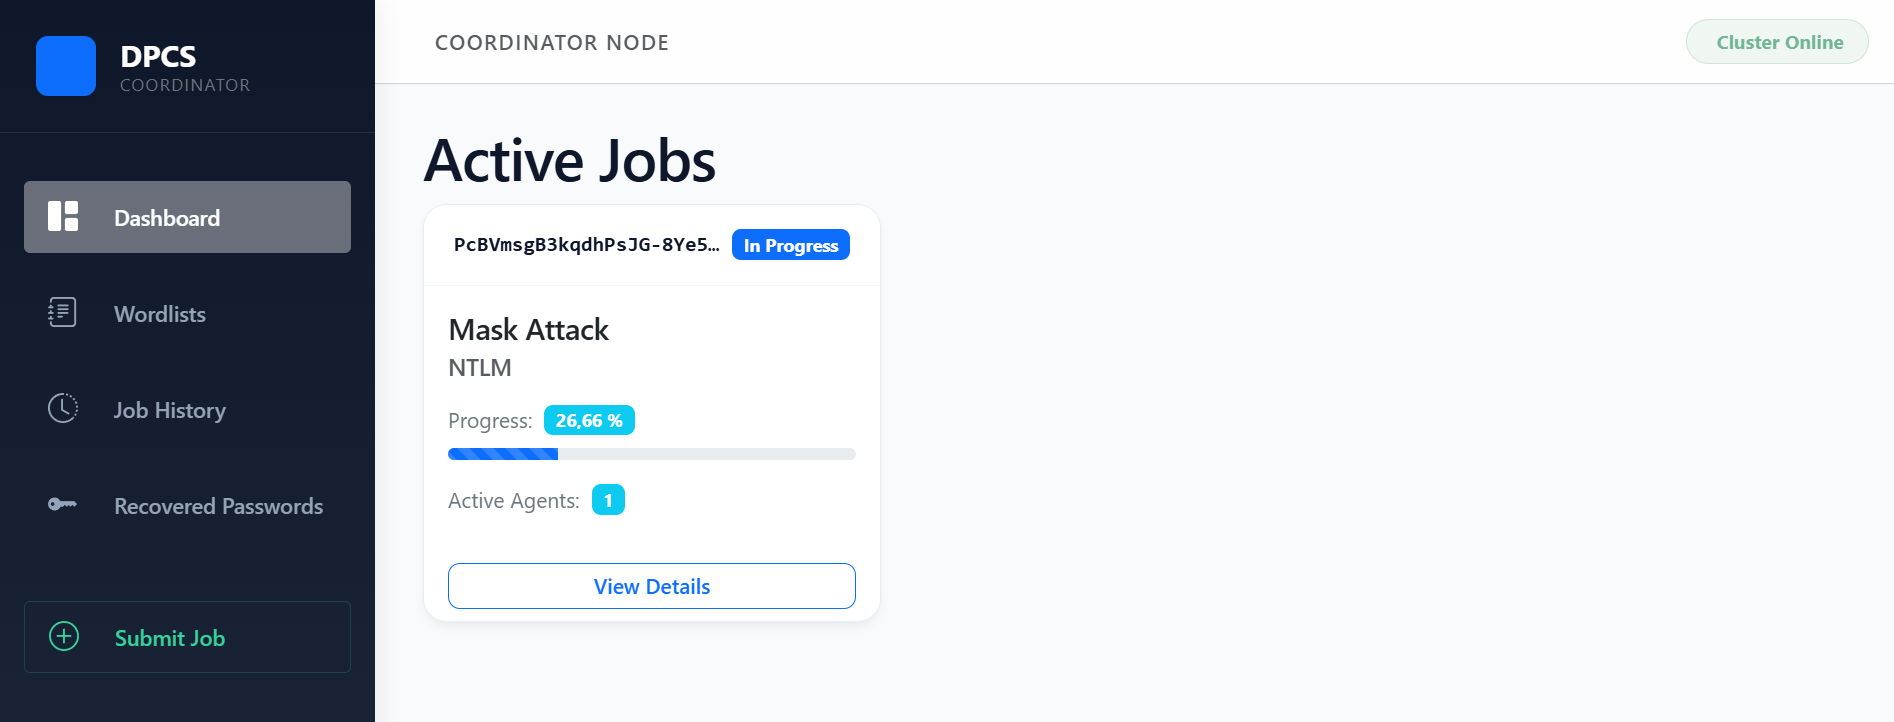
\includegraphics[width=1.0\textwidth]{obrazky-figures/dashboard.png}
    \caption{Screenshot of the Blazor Server application web interface Dashboard page, where an overview of all running jobs can be monitored.}
    \end{figure}
    
    \item \textbf{Job Submission Interface}: The creation of new cracking tasks is handled through the \verb|SubmitJob| page, which is backed by a strongly validated view model and a set of shared input controls. The user can specify the attack mode, the hash type, the target hashes (which can be entered manually or uploaded from a \textit{.hashes} or \textit{.txt} file), the chunk time, and the attack-specific parameters such as masks, wordlists, custom character sets, and optional rules. Upon form submission, the page calls the \verb|JobManagerGrain| directly through the embedded Proto.Actor cluster instance, which then persists the job and starts the corresponding Coordinator logic.

    \begin{figure}[H]
    \centering
    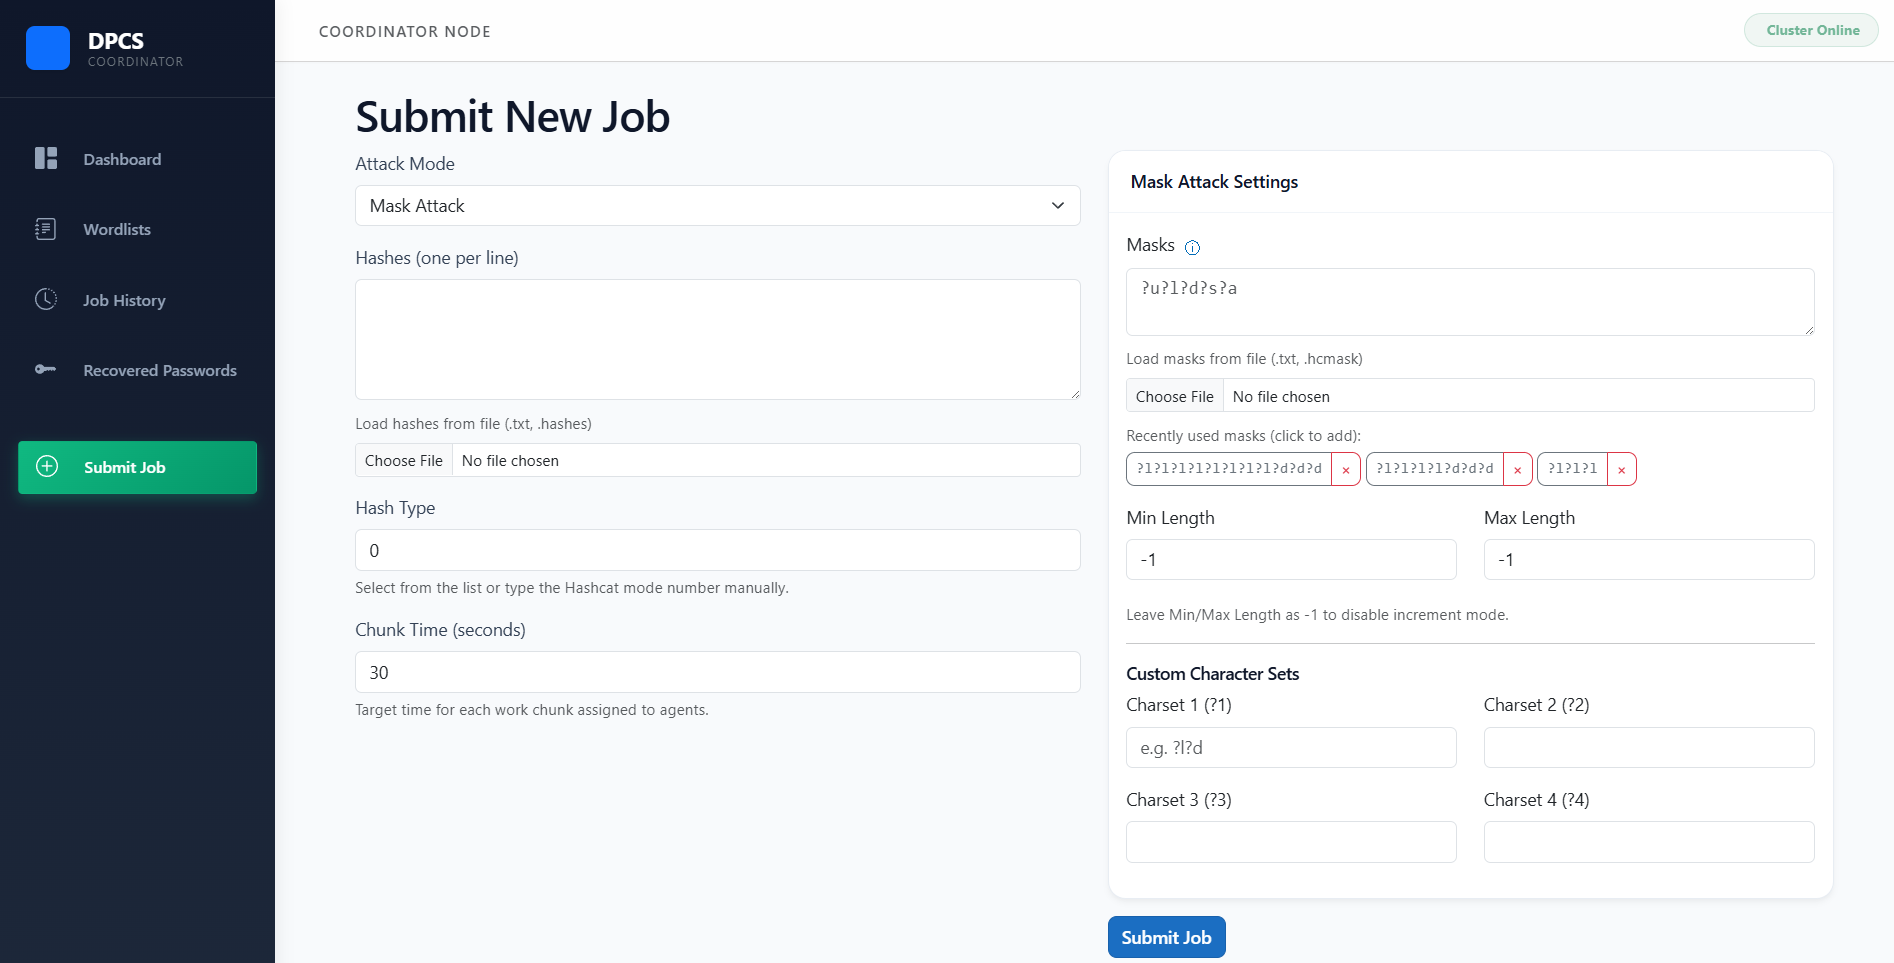
\includegraphics[width=1.0\textwidth]{obrazky-figures/mask-submit.png}
    \caption{Screenshot of a \textbf{Mask Attack} submission page, where the UI presents form fields to define the exact collection of masks to use in the attack, the custom character sets, and length increments. It also includes the ability to load previously used masks or upload masks from a \textit{.hcmask} or \textit{.txt} file.}
    \end{figure}

    \begin{figure}[H]
    \centering
    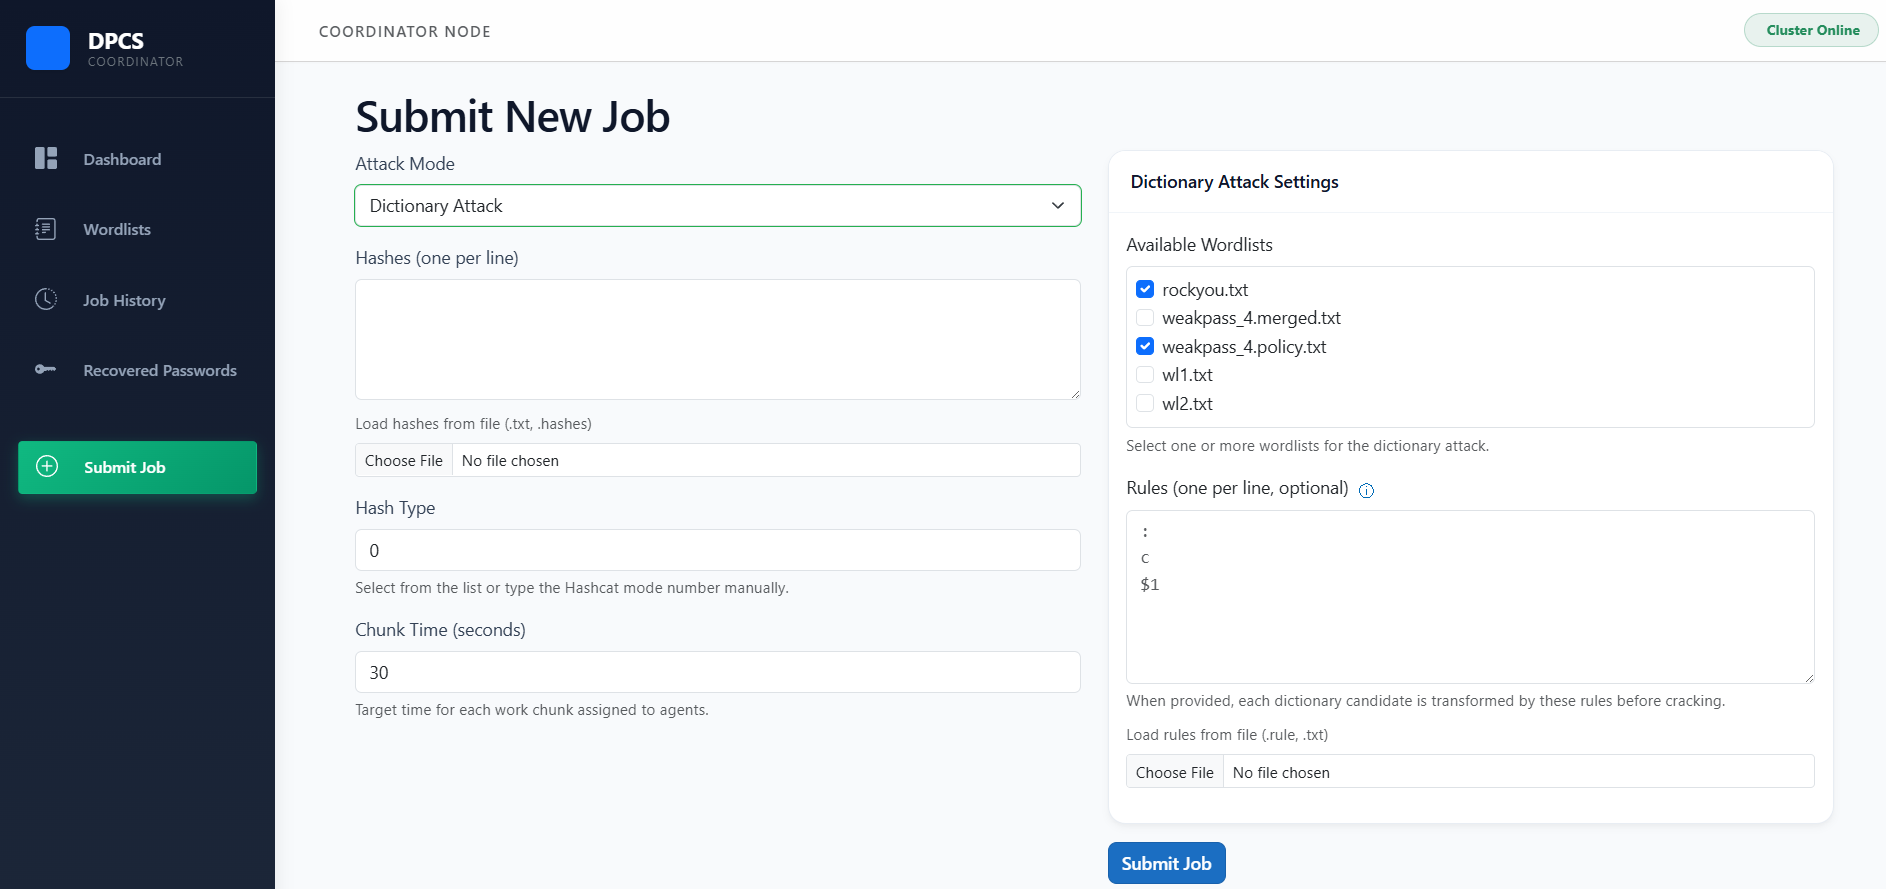
\includegraphics[width=1.0\textwidth]{obrazky-figures/dict-submit.png}
    \caption{Screenshot of a \textbf{Dictionary Attack} submission page, where the user selects one or more wordlists managed by the system. It also includes the ability to use rules to modify the wordlists, which can entered manually or uploaded from a \textit{.rule} or \textit{.txt} file.}
    \end{figure}
    
    \begin{figure}[H]
    \centering
    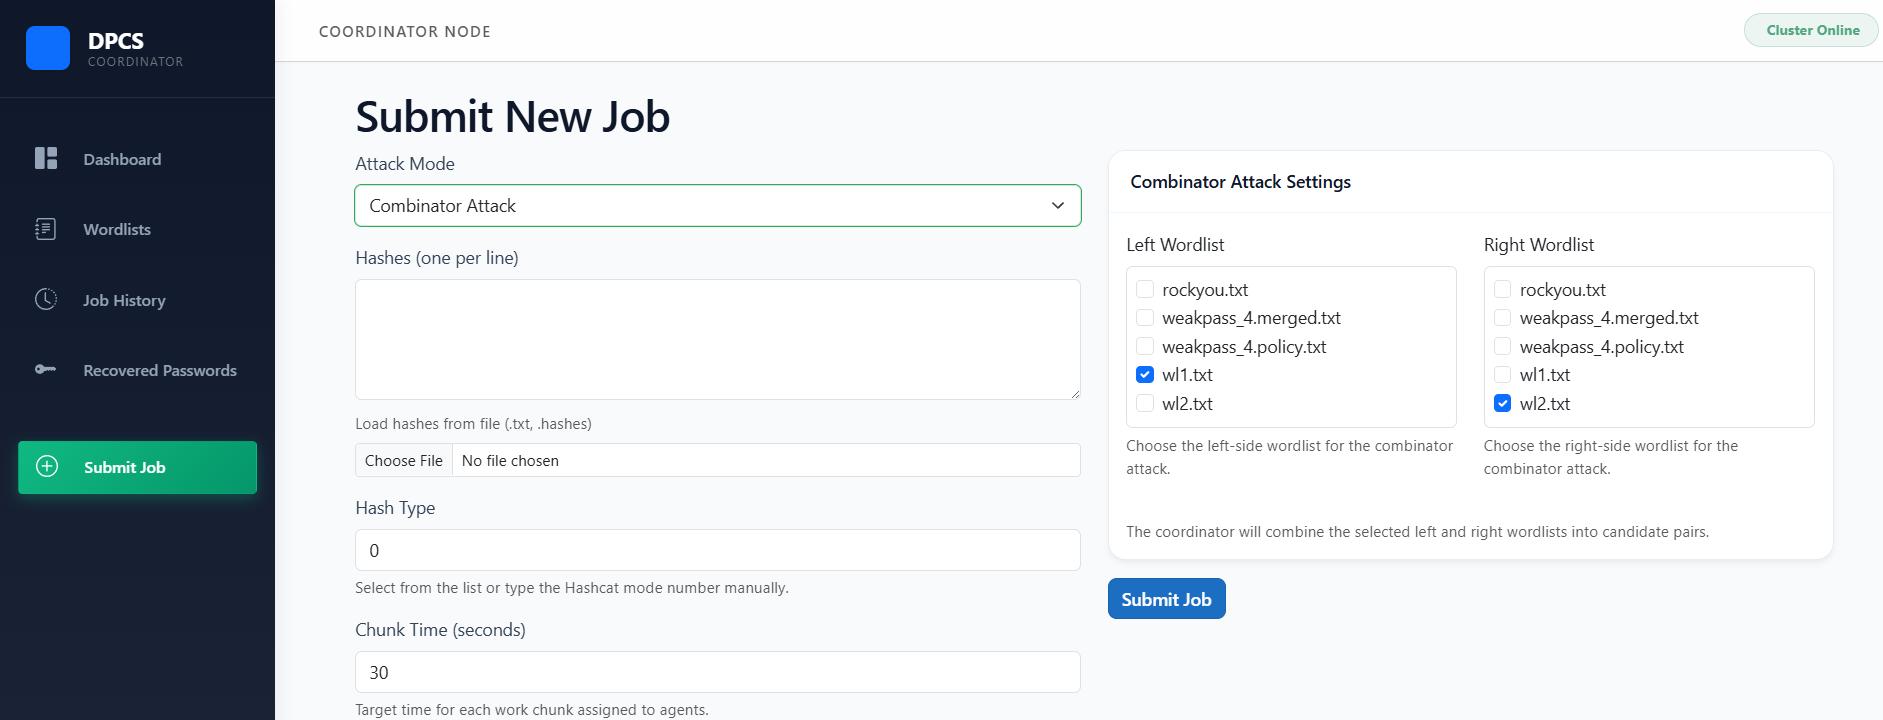
\includegraphics[width=1.0\textwidth]{obrazky-figures/combinator-submit.png}
    \caption{Screenshot of a \textbf{Combinator Attack} submission page, where the user selects one or more wordlists to be used on the left and or the right side from which the Cartesian product of password candidates is created.}
    \end{figure}

    \begin{figure}[H]
    \centering
    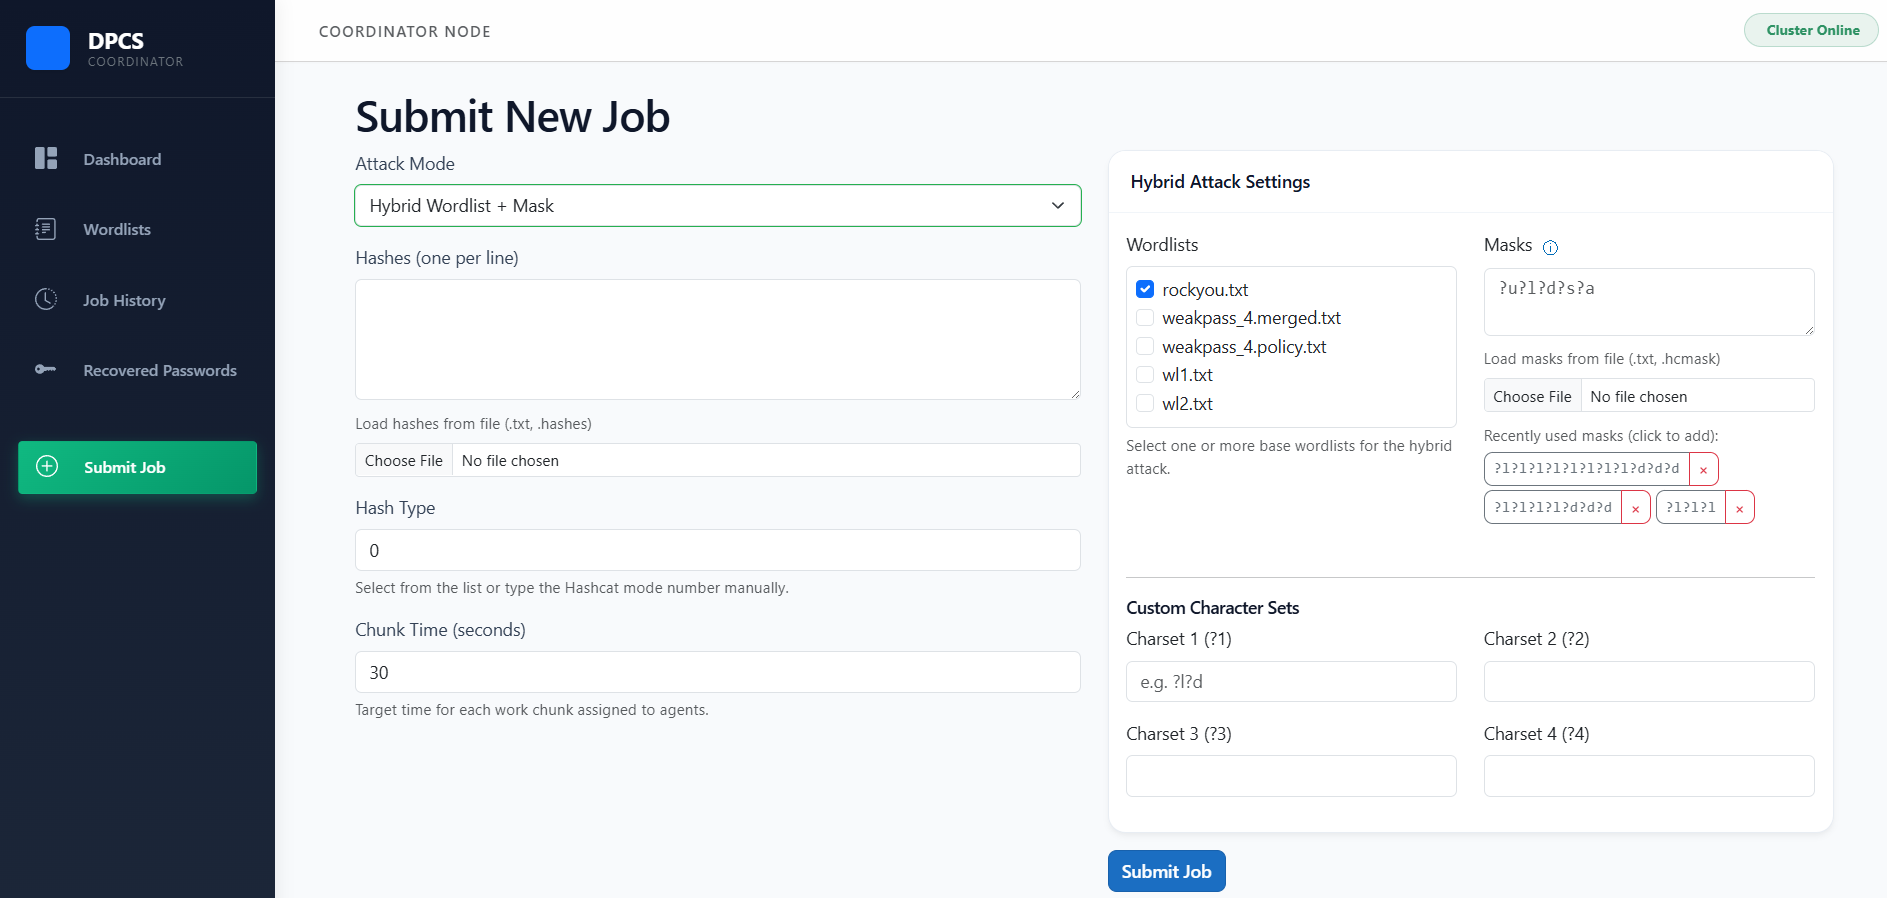
\includegraphics[width=1.0\textwidth]{obrazky-figures/hybrid-submit.png}
    \caption{Screenshot of a \textbf{Hybrid Attack} submission page, which comes in both variations for \textit{Mask + Wordlist} or \textit{Wordlist + Mask} modes based on whether the masks should be prepended or appended to the wordlist.}
    \end{figure}

    
    \item \textbf{Job Details View}: The \verb|JobDetails| page presents the original job configuration, the recovered plaintexts, the execution progress, and several shared components, including \verb|ActiveAgentsCard| for currently active Agent telemetry and \verb|AttackReportCard| for aggregated statistics and chart rendering. Because it can resolve both live job states from the actor system and historical ones from PostgreSQL, it is used for both active jobs and previously completed runs.

    \begin{figure}[H]
    \centering
    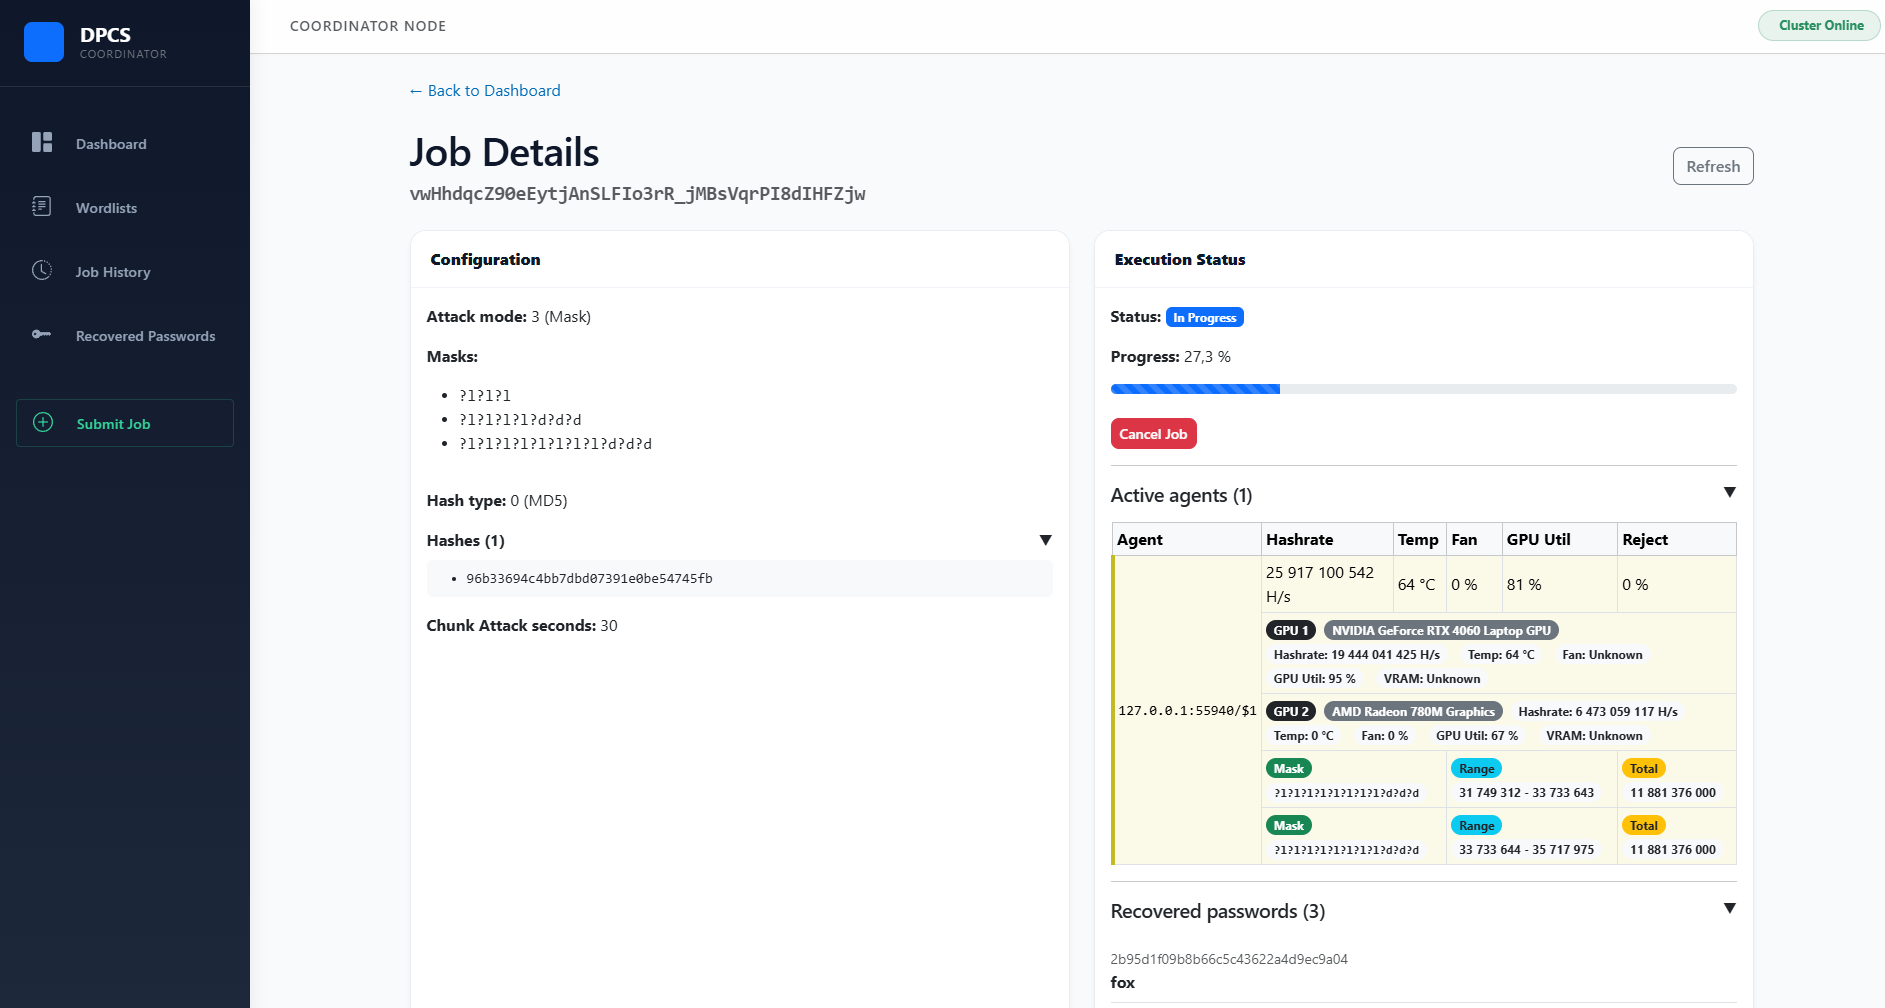
\includegraphics[width=1.0\textwidth]{obrazky-figures/attack-detail.png}
    \caption{Screenshot of a job detail page, which displays all information about the current progress of the running attack or a completed job, including assigned Agents currently cracking work chunks and their GPU metrics.}
    \end{figure}
    
    \item \textbf{Wordlist Management}: The \verb|Wordlists| page is a dedicated administrative interface for managing the dictionary files used by the cracking jobs. Users can upload wordlists, optionally overwrite existing files when no active job references them, and inspect the list of available files. The page also exposes the binary index generation mechanism used by the Manager to support HTTP byte-range downloads later during assignment execution. The index files are automatically generated upon upload, as described by Section \ref{sec:wordlist_indexing}.

    \begin{figure}[H]
    \centering
    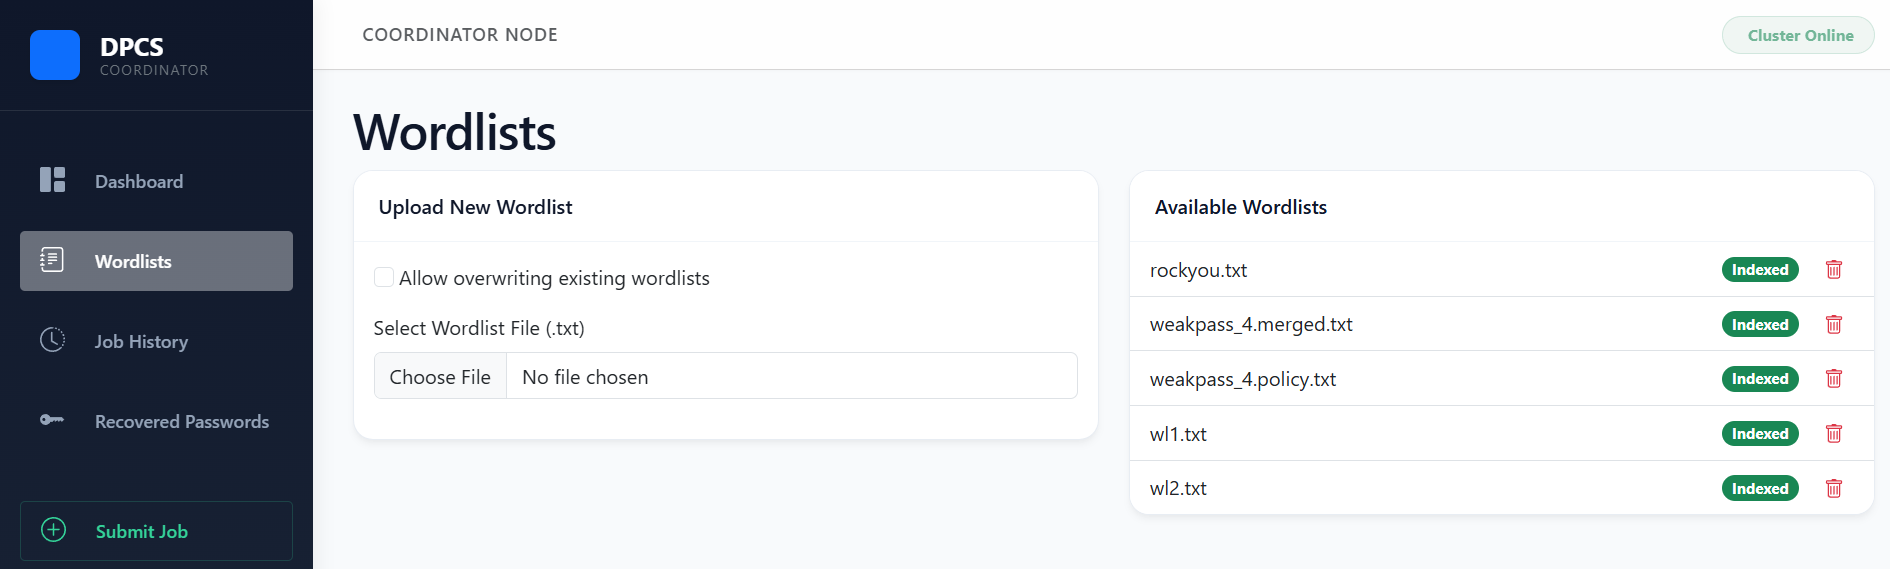
\includegraphics[width=1.0\textwidth]{obrazky-figures/wordlists-page.png}
    \caption{Screenshot of the wordlists page, where new wordlists can be uploaded and a list of already uploaded and indexed files is displayed on the right. The upload form also includes the option to allow or disable the option to overwrite existing wordlist files.}
    \end{figure}

    \item \textbf{Job History}: The \verb|JobHistory| page provides a chronological archive of completed and canceled jobs by querying the EF Core-backed PostgreSQL database. Unlike the dashboard, which emphasizes liveness and immediate progress, this page focuses on persistence, historical inspection, and navigation to the corresponding details page for each job that ran in the past.

    \begin{figure}[H]
    \centering
    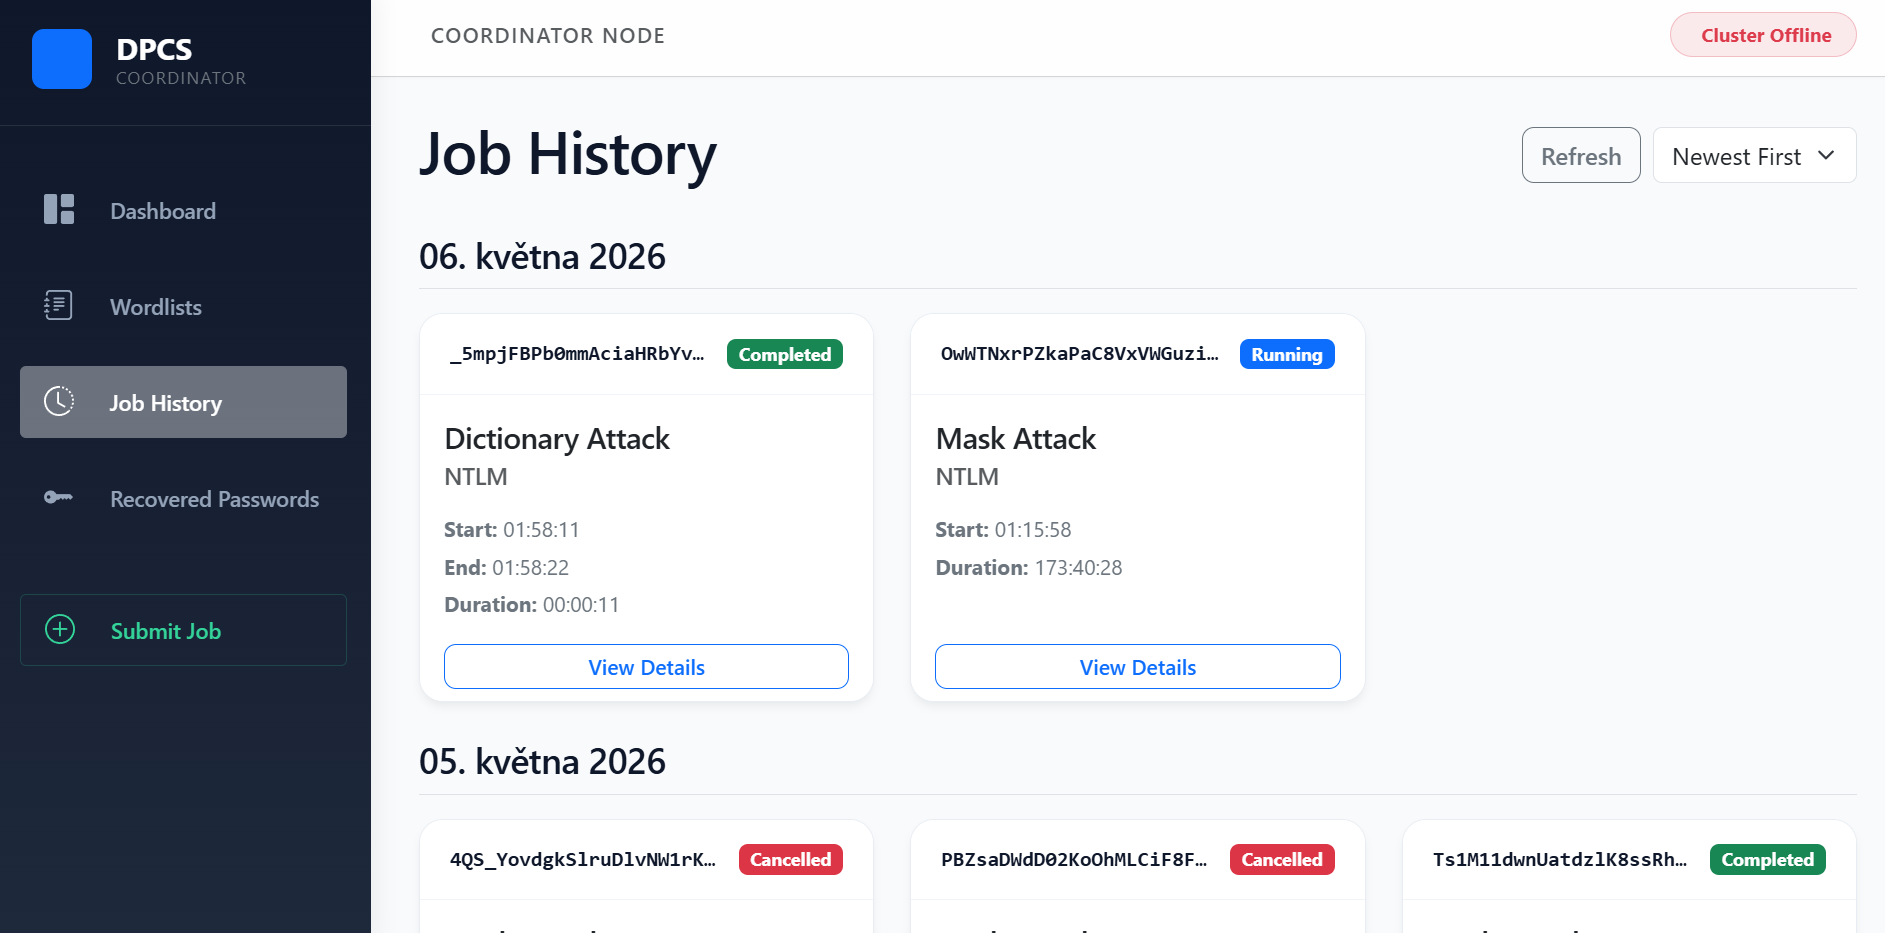
\includegraphics[width=1.0\textwidth]{obrazky-figures/job-history-page.png}
    \caption{Screenshot of the Job History page, where an overview of past cracking job runs can be viewed, leading to their detail pages.}
    \end{figure}

    \item \textbf{Recovered Passwords}: The \verb|RecoveredPasswords| page offers a centralized view of all plaintext results recovered during previous jobs. It is intentionally separated from the per-job details view so that an operator can quickly search, review, and compare recovered credentials across the full history of the cluster without navigating through each individual job.

    \begin{figure}[H]
    \centering
    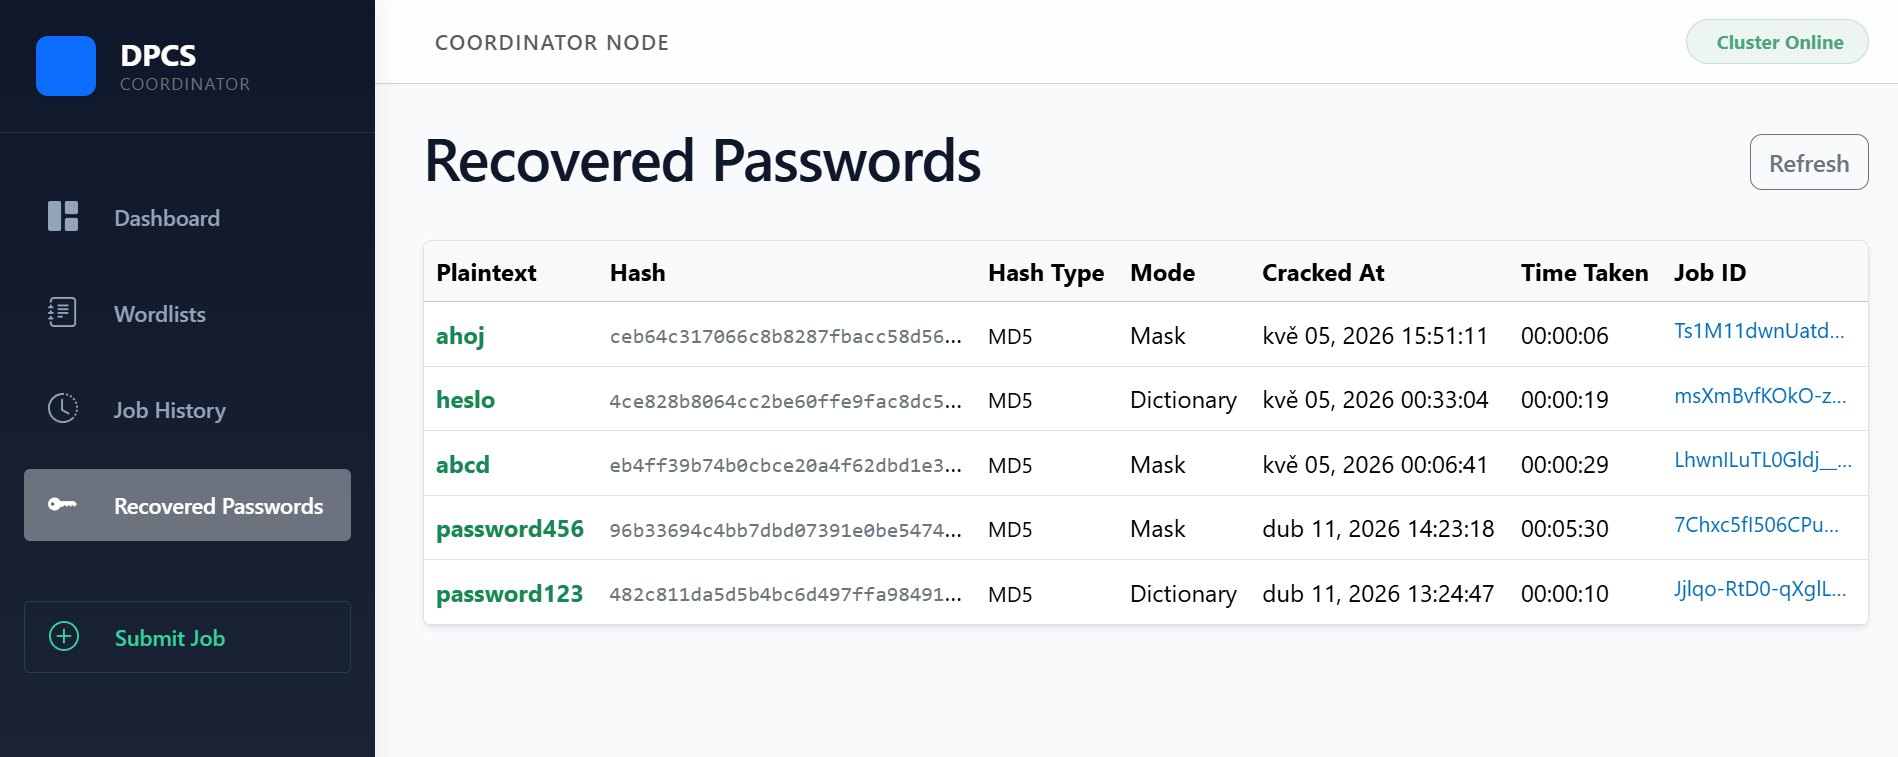
\includegraphics[width=1.0\textwidth]{obrazky-figures/rec-passwords-page.png}
    \caption{Screenshot of the Recovered Passwords page, where all past successfully cracked passwords are visible in plaintext form, accompanied by basic details.}
    \end{figure}

\end{itemize}

\subsection{Reusable Shared Components}
\label{sec:shared_components}

To adhere to the DRY (Don't Repeat Yourself) software engineering principle and maintain a cohesive design system, the Blazor application relies heavily on modular UI encapsulation. Complex or frequently used interface elements are isolated into standalone, parameter-driven Razor components within the \verb|DPCS.Blazor/Components/Shared| directory and are then composed into the higher-level pages. This design keeps the pages focused on orchestration and navigation, while the shared components handle the display of recurring state, such as job summaries, live Agent metrics, and attack-specific configuration fields.

\begin{itemize}

    \item \textbf{Job Card}: A reusable summary component used on the \textbf{dashboard} and the \textbf{job history} page. It renders the shortened job identifier, the selected attack mode, the status badge, the progress bar, and the elapsed execution time. Because the same component is instantiated from both live actor state and persisted database records, it ensures that the UI has a consistent visual language for both active and historical jobs.


    \item \textbf{Cluster Status Badge}: A persistent indicator placed in the shared application layout that displays the cluster health at a glance. It is rendered on every page and therefore provides administrators with an immediate overview of the system state without requiring them to open the full dashboard. The badge obtains its counts of Agents and Coordinators present in the cluster from the Proto.Actor membership list by calling \verb|ActorSystem.Cluster()?.MemberList?.GetAllMembers()| and counting members whose kinds contain \verb|JobCoordinatorGrain|, while the number of Agent nodes is derived from the total number of members minus the Coordinator count and the manager entry. The values are refreshed periodically so that the badge remains consistent with the live cluster composition.

    \begin{figure}[H]
    \centering
    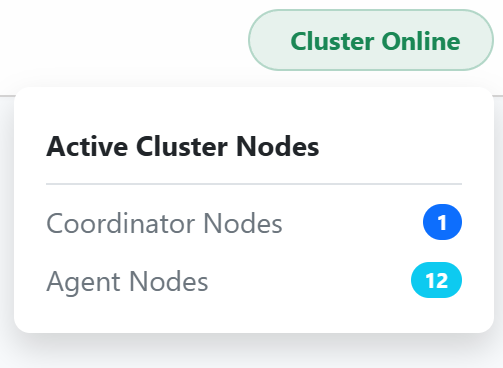
\includegraphics[width=0.33\textwidth]{obrazky-figures/cluster-badge.png}
    \caption{The cluster status badge shown in the shared layout, indicating whether the Coordinator and Agent nodes are currently reachable.}
    \end{figure}


    

    \item \textbf{Mask Selection}: The \verb|MaskSelection| component is used in the submission form to collect one or more mask expressions for a mask-style attack. It provides a textarea for direct editing, supports loading masks from a local file, and includes a small help modal that explains the built-in Hashcat charsets and the custom placeholder notation. A practical convenience feature is the list of previously used masks, which is stored by the service layer and displayed as clickable buttons so that an operator can reuse a familiar pattern without retyping it.


    \item \textbf{Wordlist Selection}: The \verb|WordlistSelection| component is composed of a selectable list of uploaded wordlists that can be used for dictionary, combinator, and hybrid attacks. Depending on the parameters passed to the component, it can render a single-select dropdown or a multi-select checklist. The component also handles the empty-state message when no dictionaries have been uploaded yet, and therefore encourages the operator to manage wordlists from the dedicated wordlist page before starting a job.


    \item \textbf{Rules Selection}: The \verb|RulesSelection| component offers an editable text area for rule content and supports loading rules from a local file. It is designed for dictionary-based attacks in which rules are applied before hashing. In addition to the input field itself, it includes a dedicated help modal with a compact reference table of common Hashcat rules, which helps operators avoid syntax mistakes while preparing a new attack and defining rules manually.


    \item \textbf{Custom Charset Controls}: The \verb|CustomCharsetFields| component provides four input fields for defining custom character sets, which can be referenced by the mask syntax using \verb|?1| to \verb|?4|. The component can operate in either editable or read-only mode, making it useful both during \textbf{job submission} and when the configuration is later displayed in a read-only \textbf{job details} view. The values are passed back to the parent form through standard Blazor event callbacks, keeping the component reusable and lightweight.


    
    

    \item \textbf{Active Agents Card}: A live view embedded into the \textbf{job details} page that displays each participating Agent together with its current hashrate, temperature, fan speed, GPU utilization, and any currently assigned work chunk. The component iterates over the \verb|JobStatus.Agents| collection, renders one table section per Agent, and uses a generated HSL-based color palette to visually distinguish individual rows. Its stylesheet, defined in \verb|ActiveAgentsCard.razor.css|, provides compact block styling and a hover effect for the table rows. The component also evaluates the \verb|AssignedChunk.PayloadCase| property to decide which chunk-specific details to display, rendering dictionary, association, mask, combinator, or hybrid information in a type-appropriate form.
\begin{comment}
    \begin{figure}[H]
    \centering
    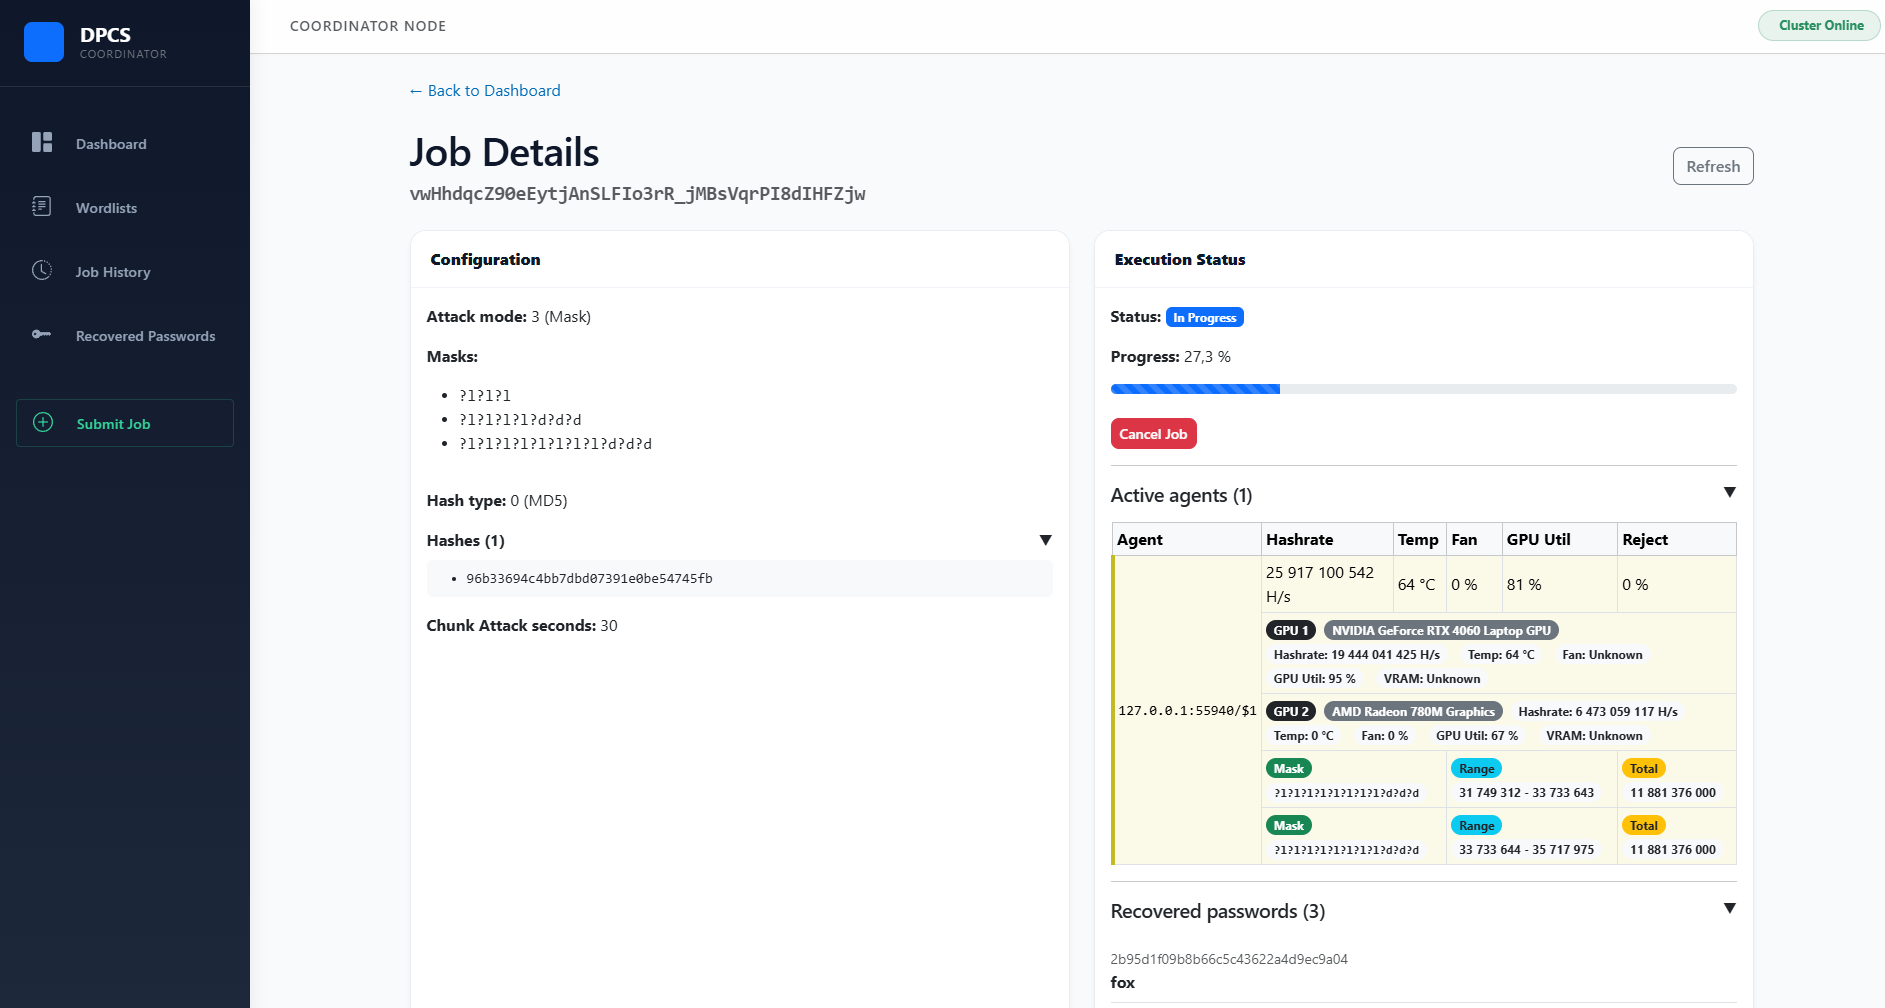
\includegraphics[width=0.95\textwidth]{obrazky-figures/attack-detail.png}
    \caption{The Active Agents card in the job detail view, showing per-Agent telemetry and assigned chunk information.}
    \end{figure}
\end{comment}

    \item \textbf{Attack Report Card}: A more elaborate reporting component included at the bottom of the \textbf{job details} page that aggregates lifecycle data and renders a large set of tables and charts. It includes summaries of coverage, completion rates, per-Agent contributions, and detailed chunk-level histories. The component is responsible for presenting the data produced by the reporting pipeline and for exposing download links for both CSV/JSON exports and PNG charts, which are later presented in the laboratory experiments of Section \ref{sec:gpu_tests}.

    \begin{figure}[H]
    \centering
    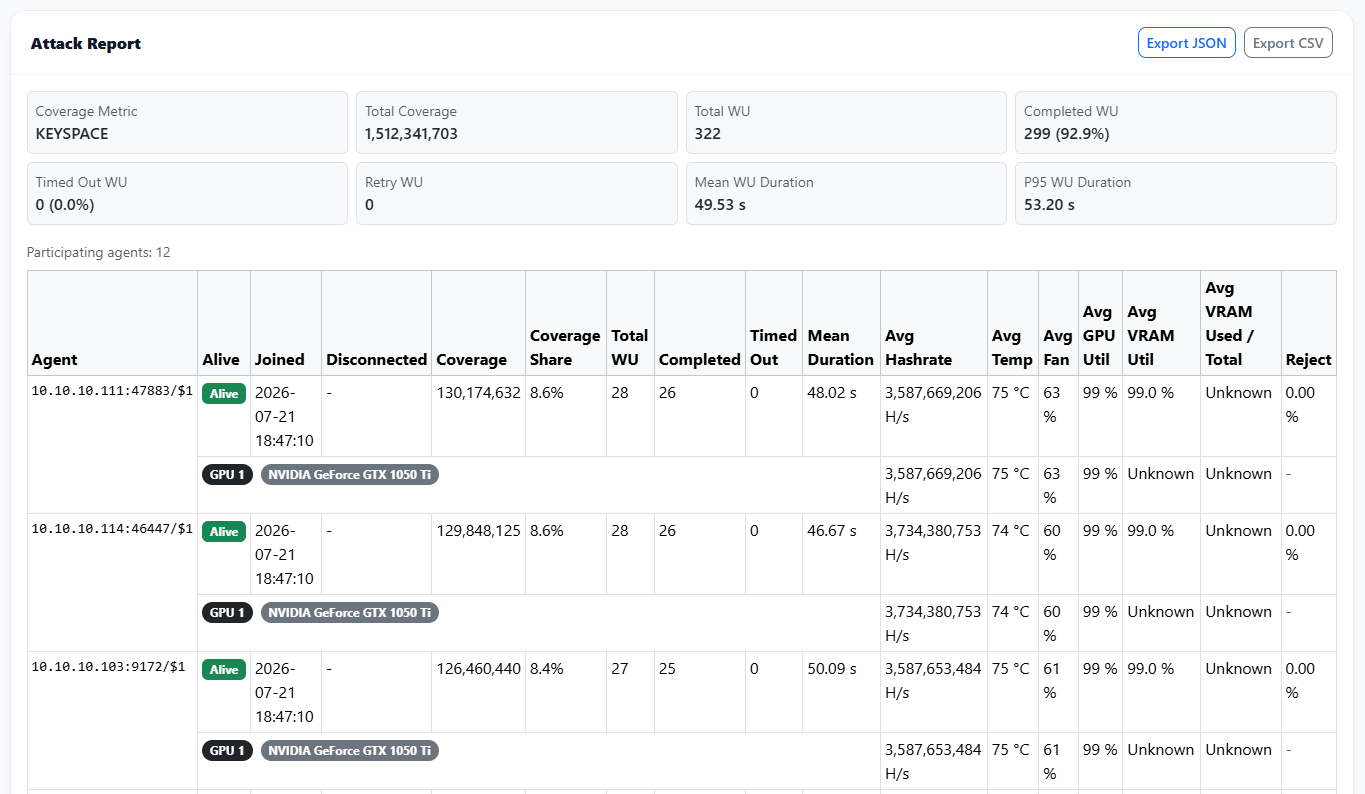
\includegraphics[width=0.95\textwidth]{obrazky-figures/attack-report.png}
    \caption{The attack report area shown in the job details view, where aggregated progress and telemetry information is presented.}
    \end{figure}

    \begin{figure}[H]
    \centering
    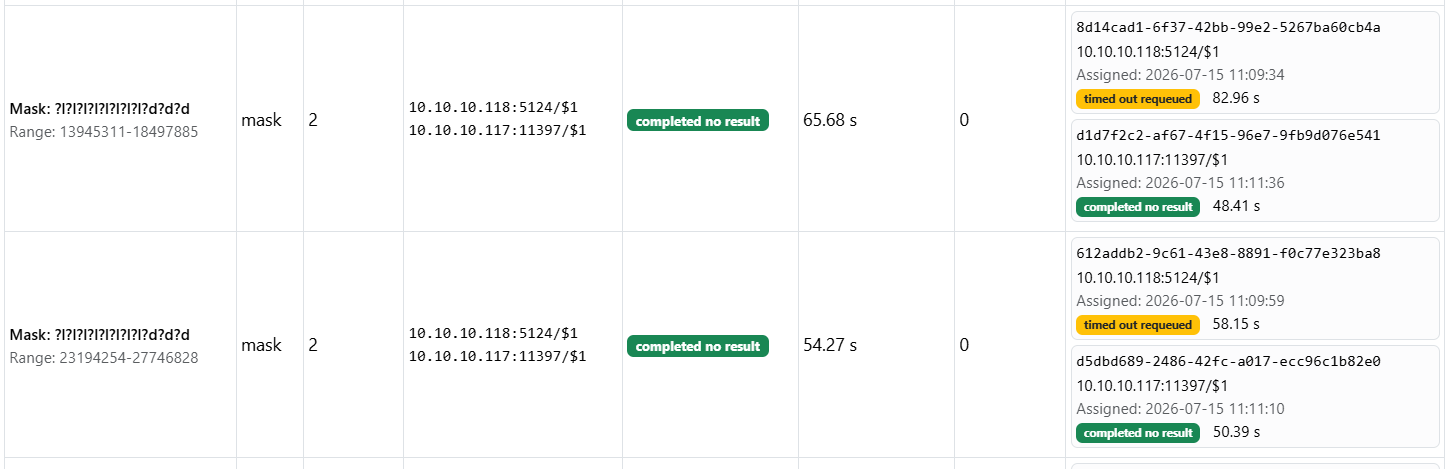
\includegraphics[width=0.95\textwidth]{obrazky-figures/attack-report-wus.png}
    \caption{The attack report component also includes information about individual Work Units, like the assigned keyspace or byte range, which Agent node it was assigned to, number of recovered passwords, and if an Agent node failed, when it was requeued to another.}
    \end{figure}



\end{itemize}

\begin{comment} \verb|/api/wordlists/{fileName}/checksum|, returns a SHA-256 checksum for an arbitrary byte range of a stored wordlist, enabling the Coordinator and the Agent-side materialization layer to verify chunk integrity without transferring the entire file. \end{comment}

\subsection{Supporting API Endpoints}

The Blazor Server also allows for the definition of a small but important set of ASP.NET Core minimal API HTTP endpoints for machine-readable access to the reporting and wordlist subsystems. These endpoints are declared in \verb|Program.cs| and are consumed directly by the Razor components.

\begin{enumerate}
    \item \verb|/api/jobs/{jobId}/work-units|: exposes the current Work Unit lifecycle export in either JSON or CSV format, which is used for the detailed \textbf{attack report} and offline analysis.
    
    \item \verb|/api/jobs/{jobId}/report-chart|: serves generated chart images for a wide range of metrics, including load balancing, per-Agent and cluster hashrate over time, GPU usage and temperature trends, progress evolution, and Work Unit duration distributions.
\end{enumerate}

\begin{comment}
    , and computing chunk checksums when the UI or API needs to verify a segment of a dictionary.
\end{comment}

The services used by these endpoints are implemented in the \verb|DPCS.Blazor.Services| namespace. The \verb|WordlistService| is responsible for storing uploads under the web application's data folder, building binary index files for byte-range access, and reporting file sizes. The \verb|MaskService| stores recently used masks in a JSON file, validates them against the Hashcat character-set syntax, and supports the reuse of commonly applied masks in the submission workflow. The most elaborate of these services is \verb|JobReportExportService|, which transforms the lifecycle, telemetry, and progress-history exports received from the actor system into human-readable CSV data and PNG charts through the \verb|ScottPlot| library\cite{scottplot}. This service is the bridge between the raw runtime telemetry produced by the Coordinator and the visually interpretable reporting experience shown on the job details page.




\section{OpenTelemetry Instrumentation and Runtime Metrics}

To support both operational monitoring and the reporting views described earlier, the implementation includes an OpenTelemetry-based observability layer. The instrumentation is configured centrally in the \verb|DPCS.ServiceDefaults| project and is activated by the Blazor Manager, the Coordinator, and the Agent through the shared \verb|AddServiceDefaults()| extension. In practice, this means that the system collects application-level metrics from the .NET runtime, from ASP.NET Core request handling, and from the custom meters defined specifically for the Agent and Coordinator services. If an OTLP endpoint is configured through the environment variable \verb|OTEL_EXPORTER_OTLP_ENDPOINT|, the collected data can be exported to an external collector or monitoring backend; otherwise, the metrics remain available to the local runtime and to development tooling.

\subsection{Metrics Defined on the Agent Node}

The Agent node emits a set of custom metrics that directly observe executed Work Units and the local GPU environment. These metrics are defined in the \verb|DPCS.Agent| project and are created with the \verb|System.Diagnostics.Metrics| API.

\begin{itemize}
    \item \verb|dpcs.Agent.hashrate|: an observable gauge that reports the current aggregate Hashcat hashrate of the local node. The value is read directly from the \verb|HashcatWrapper| and reflects the recent throughput of the running cracking process.

    \item \verb|dpcs.Agent.gpu.temperature|: an observable gauge for the average GPU temperature of the current machine.

    \item \verb|dpcs.Agent.gpu.fanspeed|: an observable gauge for the average GPU fan speed.

    \item \verb|dpcs.Agent.gpu.utilization|: an observable gauge for the average GPU utilization percentage.

    \item \verb|dpcs.Agent.reject_rate|: an observable gauge for the percentage of rejected shares reported by the local Hashcat process.

    \item \verb|dpcs.Agent.gpu.device.hashrate|, \verb|dpcs.Agent.gpu.device.temperature|,
    
    \verb|dpcs.Agent.gpu.device.utilization|, \verb|dpcs.Agent.gpu.device.vram.used|,
    
    and \verb|dpcs.Agent.gpu.device.vram.total|: per-device observable gauges that are emitted for each detected GPU. They are tagged with the device index and device name, allowing the metrics backend to distinguish the behavior of individual hardware units if more than one GPU is present in the system.

    \item \verb|dpcs.Agent.wu.started.total|: a counter incremented whenever the Agent begins execution of a new work unit. The metric is tagged with the work-unit mode, which allows the system to separate mask, dictionary, combinator, hybrid, and association traffic.

    \item \verb|dpcs.Agent.wu.result.total|: a counter incremented when a work unit finishes, with an \verb|outcome| tag that distinguishes completed, faulted, and submission-failed outcomes.

    \item \verb|dpcs.Agent.wu.active|: an up-down counter that tracks the number of work units currently executing on the Agent. The value is increased when execution starts and decreased once the work unit completes or fails.

    \item \verb|dpcs.Agent.wu.compute.duration.seconds|: a histogram metric that records the time spent in the Hashcat compute phase for each work unit.

    \item \verb|dpcs.Agent.wu.submission.duration.seconds|: a histogram that records the time spent submitting the work-unit result back to the Coordinator.

    \item \verb|dpcs.Agent.wu.total.duration.seconds|: a histogram that measures the total duration of a work-unit cycle, including both compute and submission time.
\end{itemize}

These Agent-side metrics are collected from two main sources. The gauges are sourced from the \verb|HashcatWrapper|, which exposes the current hardware and process state, while the work-unit counters and histograms are emitted by the \verb|WorkerActor| during the lifecycle of each chunk execution.

\subsection{Metrics Defined on the Coordinator Node}

The Coordinator node emits a second set of metrics that characterize how work is assigned, completed, retried, and timed out. These metrics are defined in the \verb|DPCS.Coordinator| project, inside the \verb|JobCoordinatorGrain| implementation, which is the central component responsible for orchestrating chunk execution and tracking the state of active jobs.

\begin{itemize}
    \item \verb|dpcs.Coordinator.wu.assigned.total|: a counter that increments whenever a work unit is assigned to an Agent.

    \item \verb|dpcs.Coordinator.wu.completed.total|: a counter that increments whenever a work unit is successfully completed and submitted by the Agent.

    \item \verb|dpcs.Coordinator.wu.retried.total|: a counter that increments whenever a work unit is queued for retry after a timeout or liveness expiration.

    \item \verb|dpcs.Coordinator.wu.timeout.total|: a counter that increments when a work unit times out because the assigned Agent no longer responds.

    \item \verb|dpcs.Coordinator.wu.active|: an up-down counter that tracks the number of work units currently assigned and awaiting a final result.

    \item \verb|dpcs.Coordinator.wu.processing.duration.seconds|: a histogram that records the elapsed time from assignment to completion or timeout. This metric is useful for evaluating the latency of the coordination layer and the degree to which work units are being processed within the expected time window.
\end{itemize}

The Coordinator-side metrics are collected from the job orchestration workflow itself. Each assignment, completion, retry, and timeout event is emitted by the Coordinator grain as the actor advances through the work lifecycle. In addition, the same component also records Agent presence and telemetry history, which are then used by the reporting views and chart endpoints described in the previous section.

\subsection{Manager and Shared Service Instrumentation}

The Manager node, implemented by the Blazor project, does not define its own custom metric instruments. Instead, it relies on the shared OpenTelemetry configuration provided by \verb|DPCS.ServiceDefaults|. That configuration registers ASP.NET Core instrumentation, HTTP client instrumentation, and the .NET runtime instrumentation, and it enables the \verb|DPCS.Agent| and \verb|DPCS.Coordinator| meters so that the telemetry pipeline covers the distributed system as a whole.

%From the perspective of the Manager, the most relevant metrics are therefore the framework-level measurements produced by the web server itself, including request throughput, HTTP response durations, and runtime health signals. These metrics are collected from the ASP.NET Core pipeline and from outgoing HTTP requests made by the Manager application. Because the Blazor host is also the entry point for the web UI and exposes the reporting endpoints, this instrumentation is useful for understanding the operational overhead of the management layer without requiring a separate custom metrics implementation.

\section{Deployment and Application Startup}

The current implementation is organized around two practical startup modes. The first is intended for local development and interactive testing, while the second is intended for deployment on an actual local network where the Manager, Coordinator, and Agent nodes are spread across different machines.

\subsection{Local Development with .NET Aspire}

For local development, the preferred entry point is the Aspire AppHost project. \textbf{Docker} needs to be running in the background before launching. The command below starts the full distributed application from a single location:

\begin{verbatim}
dotnet run --project DPCS.AppHost
\end{verbatim}

The AppHost project is responsible for defining the distributed application topology. In the current implementation, it creates a PostgreSQL database resource, adds a Consul container, and then registers the Blazor, Coordinator, and Agent projects as application resources that depend on those infrastructure services. The AppHost uses the \verb|WithReference| mechanism to provide the dependent projects with the connection string for PostgreSQL and the endpoint for the Consul container so that the applications can discover the required infrastructure without hard-coded wiring.

When the application is launched, Aspire also opens a dashboard that shows the running containers and projects, their health status, exposed endpoints, and log output. This makes it convenient to observe the whole system as one deployment unit during development. During development, the PostgreSQL container can take longer to start and initialize the database, causing the Blazor and Coordinator executables to crash because EF Core cannot run the database migration process properly. When that happens, they can be started again from the Aspire dashboard directly.

The configuration files used by the projects are still read from the standard .NET configuration pipeline. The AppHost itself does not require any custom command-line arguments for the normal development flow. The relevant values are supplied through \verb|appsettings.json| files or through environment variables and the Aspire injection mechanism.

\begin{verbatim}
// DPCS.Blazor/appsettings.json
{
  "Logging": {
    "LogLevel": {
      "Default": "Information",
      "Microsoft.AspNetCore": "Warning"
    }
  },
  "AllowedHosts": "*",
  "ProtoActor": {
    "Host": "10.10.10.118",
    "Port": 12000
  },
  "Kestrel": {
    "Endpoints": {
      "Http": {
        "Url": "http://0.0.0.0:5065"
      }
    }
  }
}
\end{verbatim}

\begin{verbatim}
// DPCS.Coordinator/appsettings.json
{
  "Logging": {
    "LogLevel": {
      "Default": "Information",
      "Microsoft.AspNetCore": "Warning"
    }
  },
  "AllowedHosts": "*",
  "Hashcat": {
    "Path": "C:\\hashcat-7.1.2\\hashcat.exe"
  },
  "ConnectionStrings": {
    "dpcs": "Host=10.10.10.118;Port=5432;Database=dpcs;
                  Username=postgres;Password=password123",
    "consul-http": "http://10.10.10.118:8500"
  },
  "ProtoActor": {
    "Host": "10.10.10.118",
    "Port": 12001
  },
  "DPCS": {
    "ServerBaseUrl": "http://10.10.10.118:5065"
  }
}
\end{verbatim}

\begin{verbatim}
// DPCS.Agent/appsettings.json
{
  "Hashcat": {
    "Path": "C:\\hashcat-7.1.2\\hashcat.exe",
    "WorkloadProfile": 2
  },
  "ConnectionStrings": {
    "consul-http": "http://10.10.10.118:8500"
    },
  "ProtoActor": {
    "Host": "10.10.10.103",
    "Port": 0
  }
}
\end{verbatim}

For the local setup, the most important values are the Proto.Actor host and port, the Hashcat executable path, and the web server base URL used by the Coordinator. In a development environment, they are often left at loopback values (127.0.0.1), but the same configuration can be adapted to a private LAN by inputting the actual IP address of the relevant machine.

\newpage

\subsection{Deployment on a Real Local Network}

When the system is deployed on a real local network, the Manager, Coordinator, and Agent nodes are started as ordinary .NET applications. In this case, only the workstation hosting the Manager node needs to have \textbf{Docker} running in the background, as it is responsible for launching the Consul and PostgreSQL containers. To start them, run the following command in the directory with the provided \verb|docker-compose.yml| file:

\begin{verbatim}
docker-compose up -d
\end{verbatim}

Then, all nodes are launched in the same manner in separate terminal windows:

\begin{verbatim}
dotnet run --project DPCS.Blazor
dotnet run --project DPCS.Coordinator
dotnet run --project DPCS.Agent
\end{verbatim}

For environments where the Agent is expected to run on different machines, the Agent project can also be published and started from the generated output directory. This approach was utilized while performing laboratory tests in Section \ref{sec:gpu_tests} in the next chapter by simply copying the published directory with DLL files and \verb|appsettings.json| from a flash drive onto each workstation's disk. The publish step is shown below:

\begin{verbatim}
dotnet publish .\DPCS.Agent\DPCS.Agent.csproj -c Release
\end{verbatim}

After publishing, the executable can be launched directly from the published directory as follows:

\begin{verbatim}
dotnet DPCS.Agent.dll
\end{verbatim}

In this deployment mode, the configuration values must be adjusted to match the actual network topology. The Manager node should expose its web UI using the 0.0.0.0 IP address and host the Consul service that the other nodes use for discovery by using its own IP address. The Coordinator and Agent projects should point to the Manager node's address through the relevant configuration values, while each node should also publish its own reachable Proto.Actor \verb|Host| address and the \verb|Port| value (where \verb|0| allows the OS to select a dynamic port, and a fixed value can be used when a specific port must be reserved), the path to the Hashcat executable, and, where necessary, the web server base URL used by the Coordinator to reach the Manager UI. This arrangement allows the nodes to join the same cluster even when they are located on different machines in the same private network.



% =========================================
% CHAPTER 6: PERFORMANCE EVALUATION
% =========================================
\chapter{Performance Evaluation}
\label{chap:evaluation}

The value of a distributed system lies in its ability to scale efficiently, utilize hardware optimally, and survive adverse conditions. This chapter empirically evaluates the DPCS architecture using two complementary approaches: (1) deterministic in-process simulations implemented in \verb|DPCS.Tests| and (2) physical multi-node GPU experiments executed in a real laboratory environment. Together, these approaches test the design claims regarding latency hiding, dynamic load balancing, and data distribution efficiency under both controlled and real operating conditions.

\section{Methodology and the Test Environment}

Evaluating a distributed actor system requires a methodology that can reliably test multi-node orchestration, fault recovery, and dynamic load-balancing mathematics. Traditional micro-benchmarking tools are insufficient for this task because the scenarios involve complex lifecycles, hardware heterogeneity, and deliberate node termination.

The methodology used in this thesis is split into two stages. First, an \textbf{In-Process System Simulation} is used to obtain repeatable validation of the orchestrator's chunk scheduling algorithms, actor supervision trees, database concurrency, and fault-tolerance recovery logic. This was implemented in the DPCS.Tests project using the xUnit testing framework to run defined scenarios.

Second, selected scenarios are re-executed in a physical laboratory cluster to validate behavior with physical GPU telemetry and real process scheduling overhead. The results of these experiments are presented in Section \ref{sec:gpu_tests}.

\subsection{The xUnit Evaluator Harness}
Instead of relying on manual interactions in the web UI or shell scripts spawning OS processes, the testing is driven by a dedicated, automated test harness built using the \textbf{xUnit} testing framework \cite{xunit}. This approach provides strict isolation and sequential execution of performance scenarios.

To accurately test the database concurrency constraints without the friction of local installations, the evaluator utilizes the \textbf{Testcontainers} library. For every test scenario, Testcontainers \cite{testcontainers} dynamically spins up an ephemeral, disposable PostgreSQL Docker container. This guarantees a completely clean database state per test while maintaining the true Multi-Version Concurrency Control (MVCC) behavior of PostgreSQL, which an in-memory mock database cannot replicate. Additionally, the \textbf{ScottPlot} \cite{scottplot} library is integrated into the test suite to programmatically generate the evaluation charts and graphs directly from the benchmark data.

To maintain a clean and modular testing architecture, the \verb|DPCS.Tests| project is structurally partitioned into distinct components:
\begin{itemize}
    \item \textbf{Infrastructure}: Contains the \verb|ClusterTestBase| class, which ensures that a fresh PostgreSQL Docker container and an isolated in-memory Consul service mesh (by utilizing the \verb|Proto.Cluster.Testing.InMemAgent| built-in class) are established before each test and are cleanly disposed of afterward by implementing the \verb|IAsyncLifetime| interface.

    \item \textbf{Wrappers}: Houses the \verb|DummyHashcatWrapper|, a testing mock implementation of the \verb|IHashcatWrapper| interface capable of simulating varying hardware hash rates, applying precise time multipliers, and generating chunk execution metrics without invoking actual OS subprocesses.

    \item \textbf{Scenario Definitions}: Each of the performance evaluations is isolated into a dedicated class (\verb|Scenario1_LoadBalancingTests|, \verb|Scenario2_PrefetchLatencyTests|, and \verb|Scenario3_FaultToleranceTests|). This separation ensures that complex assertions involving load distribution, network latency masking, and actor supervision are decoupled and independently verifiable.
\end{itemize}

\subsection{In-Memory Clustering and Hardware Simulation}
To eliminate the dependency on a running Consul service mesh and the latency of local loopback network routing, the test harness leverages Proto.Actor's built-in \verb|TestProvider|. This provider allows the entire Manager, Coordinator, and Agent actor topology to be instantiated directly within the xUnit process memory space, simulating instantaneous cluster discovery and message routing.

Furthermore, to show that the system solves the "Straggler Problem" without needing physically different hardware, the system's architecture relies on the Dependency Inversion Principle. The raw Hashcat execution logic is abstracted behind an \verb|IHashcatWrapper| interface. Within the evaluation project, a \verb|DummyHashcatWrapper| is injected into the simulated Agent nodes. 

This dummy wrapper allows the test harness to explicitly dictate mock hashrates. By injecting Agent A with a mocked hashrate of 1,000 H/s and Agent B with 100,000 H/s, the Evaluator tricks the \verb|JobCoordinatorGrain| into calculating different keyspace bounds. The dummy wrapper then artificially delays its \verb|Task| completion based on the assigned chunk size to simulate actual cracking time.

\subsection{Simulated Test Datasets}
To expose different systemic bottlenecks within this environment, the tests emulate the behavior of two distinct cryptographic algorithms by calibrating the \verb|DummyHashcatWrapper| parameters:
\begin{itemize}
    \item \textbf{Fast Hash} (e.g. MD5, NTLM): Computationally trivial. Simulated by setting a rapid compute time parameter (e.g., 500 milliseconds per chunk). This explicitly tests the system's orchestration overhead, the impact of network latency, and the effectiveness of the prefetching queue.
    \item \textbf{Slow Hash} (e.g. bcrypt, argon2): Computationally expensive. Simulated by setting a prolonged compute time parameter (e.g., 30 seconds per chunk). This explicitly tests long-running task stability, dynamic load balancing mathematics, and exact keyspace division without network routing times skewing the results.
\end{itemize}

\begin{comment}
\subsection{Simulation Scope and Limitations}
While the in-process simulation provides absolute mathematical verification of the actor state machines, dynamic chunking logic, and fault recovery algorithms, it inherently limits the evaluation of physical data plane operations. 

Consequently, evaluating the physical network bandwidth saturation and peak RAM utilization of Agent nodes during HTTP Byte-Range distribution of multi-gigabyte dictionary wordlists (as designed in Section \ref{sec:http_range_requests}) cannot be fully concluded from simulation alone. This is why the chapter now includes real laboratory experiments in C304; however, because only one laboratory day was available, not all planned attack-mode variants were measured on physical hardware.
\end{comment}

\section{Dynamic load balancing and Hardware Heterogeneity}
As detailed in Chapter \ref{chap:analysis}, statically dividing the keyspace among cluster nodes invariably leads to the "Straggler Problem," where fast hardware sits idle waiting for slower nodes to finish disproportionately large chunks of work. To empirically validate the dynamic chunk sizing algorithms implemented within the \verb|JobCoordinatorGrain|, the system was evaluated using a heterogeneous simulated cluster.

The test spawned four \verb|WorkerActor| instances injected with the \verb|DummyHashcatWrapper| implementation, representing different capabilities:
\begin{itemize}
    \item \textbf{Agent A \& B}: Simulated low-end CPUs processing 50,000 H/s each.
    \item \textbf{Agent C}: A simulated mid-range GPU processing 100,000 H/s.
    \item \textbf{Agent D}: A simulated high-end GPU processing 200,000 H/s.
\end{itemize}

The Coordinator was instructed to orchestrate an attack over a total keyspace of 120,000,000 candidates, targeting an average \verb|ChunkTimeSeconds| of 30 seconds per work assignment.

\begin{table}[hbt]
\centering
\caption{Empirical data from a 4-node heterogeneous cluster simulation demonstrating fair workload distribution proportional to the simulated hardware capabilities of each node.}
\label{tab:load-balancing-evaluation}
\footnotesize
\begin{tabular}{|l|c|c|c|c|l|}
\hline
\textbf{Metric} & \textbf{Agent A} & \textbf{Agent B} & \textbf{Agent C} & \textbf{Agent D} & \textbf{Cluster Total} \\ 
 & (50k) & (50k) & (100k) & (200k) & \\ \hline
Assigned Chunks & 10 & 10 & 10 & 10 & 40 \\ \hline
Keyspace Covered & 15,000,000 & 15,000,000 & 30,000,000 & 60,000,000 & 120,000,000 \\ \hline
Coverage Percentage & 12.50\% & 12.50\% & 25.00\% & 50.00\% & 100\% \\ \hline
Total Compute Time & 300.00 s & 300.00 s & 300.00 s & 300.00 s & - \\ \hline
Avg Time per Chunk & 30.00 s & 30.00 s & 30.00 s & 30.00 s & - \\ \hline
\end{tabular}
\end{table}

\begin{figure}[H]
\centering
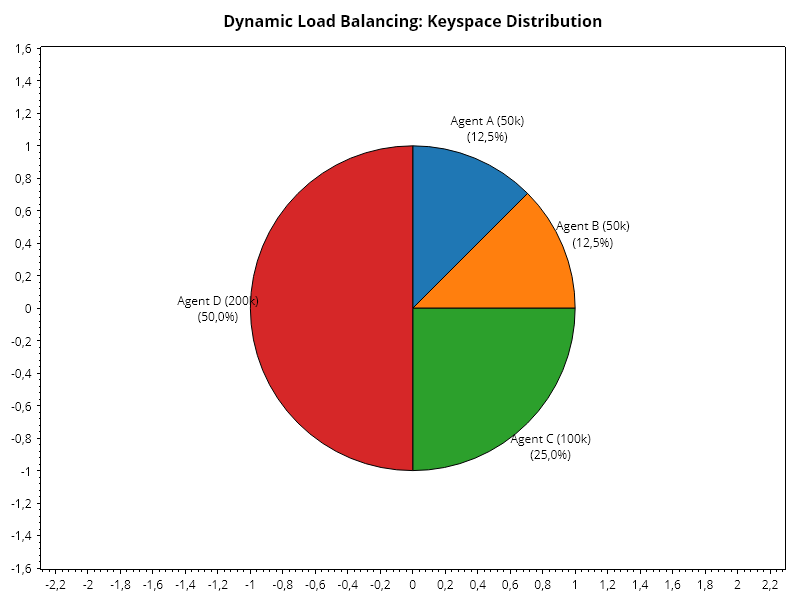
\includegraphics[width=0.8\textwidth]{obrazky-figures/LoadBalancing_Keyspace.png}
\caption{A pie chart visualization of the total keyspace distribution, matching the proportional hardware capabilities of the nodes. For example, Agent D (200,000 H/s) processed four times the keyspace of Agent A (50,000 H/s), as expected.}
\label{fig:loadbalancing-keyspace}
\end{figure}

\begin{figure}[H]
\centering
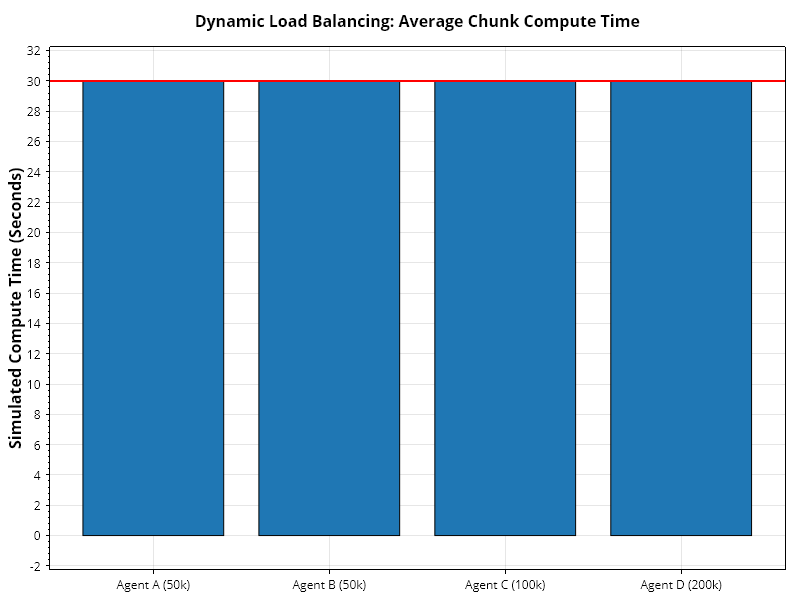
\includegraphics[width=0.8\textwidth]{obrazky-figures/LoadBalancing_TimePerChunk.png}
\caption{Average chunk time was at the 30 second target mark for all Agents, even though some of them were assigned more work than others based on their simulated hardware capabilities. This shows the expected behavior of the dynamic chunk size scheduling.}
\label{fig:loadbalancing-time}
\end{figure}

\section{Latency Hiding and Prefetch Evaluation}
As argued in Chapter \ref{chap:analysis}, network latency introduces significant overhead when cracking fast hashes. This section measures the GPU utilization percentage (via the \verb|HashcatWrapper| telemetry) under two scenarios:
\begin{enumerate}
    \item \textbf{Strict Polling (No Prefetching)}: The Agent requests a chunk, processes it, and waits idly for the next response over the network before continuing.

    \item \textbf{Event-Driven (Prefetching Enabled)}: The Agent utilizes the \verb|ReenterAfter| mechanism to fetch the subsequent chunk in the background while the GPU is actively computing the current chunk.
\end{enumerate}

To properly observe this interaction, the simulated \verb|JobCoordinatorGrain| was instrumented to inject an artificial 250-millisecond delay into every \verb|WorkRequest| to accurately represent real-world routing and database latency across a Wide Area Network (WAN). The test executed a rapid simulated attack (representing MD5) requiring exactly 10 chunks of work, with the \verb|DummyHashcatWrapper| calibrated to require approximately 500 milliseconds of compute time per chunk.

\begin{table}[hbt]
\centering
\caption{Execution times of a fast-hashing job with simulated 250 ms network latency.}
\label{tab:prefetch-evaluation}
\begin{tabular}{|l|c|l|}
\hline
\textbf{Architecture} & \textbf{Total Execution Time (s)} & \textbf{Performance Gain} \\ \hline
Polling (No Prefetch) & 7.82 & Baseline \\ \hline
Event-Driven (Prefetch) & 5.54 & +29.09 \% \\ \hline
\end{tabular}
\end{table}

\begin{figure}[H]
\centering
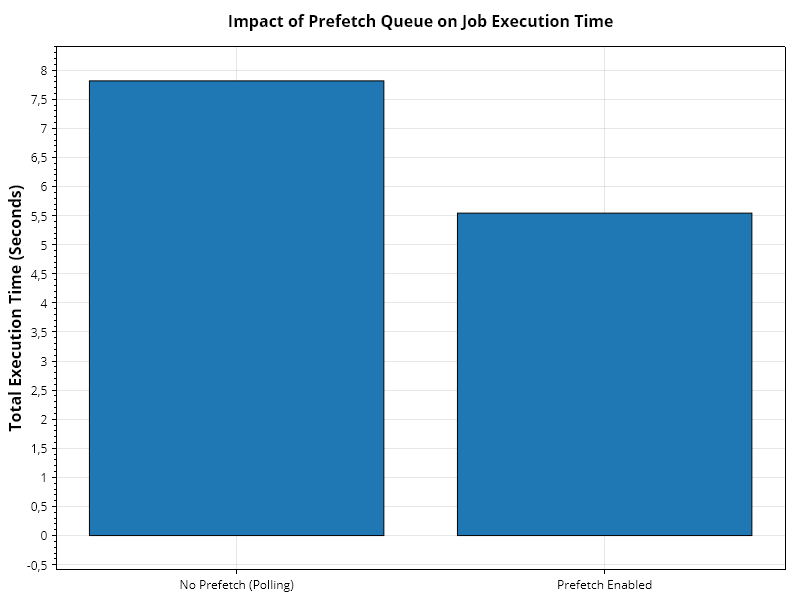
\includegraphics[width=0.8\textwidth]{obrazky-figures/Prefetch_Evaluation.png}
\caption{A bar chart visualization demonstrating the total cluster execution time reduction achieved by hiding network latency behind computational cycles.}
\label{fig:prefetch-evaluation}
\end{figure}

As shown in Table \ref{tab:prefetch-evaluation} and Figure \ref{fig:prefetch-evaluation}, the results align with the expected behavior. In the strict polling scenario, the network latency and computation time execute \textbf{sequentially}. A single cycle requires $250\text{ms} + 500\text{ms} = 750\text{ms}$. Across 10 chunks, this totals $\sim7.5$ seconds (yielding a 7.82 s simulation result, inclusive of framework instantiation overhead). The GPU remained idle 33 \% of the time, waiting for network packets.

Conversely, the event-driven prefetch architecture processed the entire workload in 5.54 seconds, achieving a near 30\% reduction in total execution time. Beyond the initial 250 ms penalty incurred during the first chunk download, the network latency was entirely masked. The node fetched chunk $N+1$ concurrently while computing chunk $N$. It is therefore expected to see near full GPU utilization in the later laboratory measurements.

\subsection{Discovery of Mailbox Congestion through Over-Fetching}
An important architectural observation was made during adjustments to the value of the \verb|MaxPrefetchQueueSize| parameter. Initially, the queue size was set to allow 2 pending chunks. In a high-latency environment, the \verb|WorkerActor| immediately dispatched two rapid, consecutive network requests to the Coordinator to fill its queue. 

Because the \verb|JobCoordinatorGrain| (like all Virtual Actors) is single-threaded to prevent state corruption, its mailbox became temporarily congested while processing these back-to-back requests, each suffering a routing delay. When the fast \verb|WorkerActor| finished computing its first chunk and attempted to submit the result, the Coordinator was still busy processing too many prefetch requests. This congestion blocked the acknowledgment of the result submission, forcing the \verb|WorkerActor| to halt execution.

This phenomenon showed that while prefetching is a useful mechanism for latency hiding, over-prefetching in an Actor Model environment creates control-plane bottlenecks. The optimal configuration discovered for fast-hashing algorithms is a strict queue size of 1, ensuring that the worker requests exactly one chunk ahead of time, maintaining a staggered pipeline without blocking the central orchestrator's mailbox.

\section{Simulating Fault Tolerance and Actor Supervision}
From the perspective of the Coordinator's liveness probe, a remote router dying or a server losing power looks identical: the periodic \verb|AgentTelemetry| heartbeats stop arriving. To empirically evaluate the "Distributed Checkpointing" mechanism described in Chapter \ref{chap:analysis}, a node failure was programmatically injected into a running cluster.

The simulation was instantiated with two Agents assigned to process a keyspace of 12,000,000 candidates, which the \verb|JobCoordinatorGrain| segmented into four chunks of 3,000,000 candidates. Due to the prefetch architecture, both Agent A and Agent B immediately checked out two chunks each. To accurately test the recovery timeline without artificial delays caused by the test's accelerated time multiplier, the heartbeat and timeout thresholds were parameterized to a 2-second interval and a 6-second timeout (compared to the production standard of 15 and 45 seconds, which prioritizes minimal network overhead).

While the Agents were actively computing their initial chunks, Agent A was terminated mid-flight. As expected, Agent B successfully finished its assigned workload and entered a standby polling loop. Because the final chunk assigned to Agent A remained unacknowledged, the global job progress stalled at 75\%.

\begin{figure}[H]
\centering
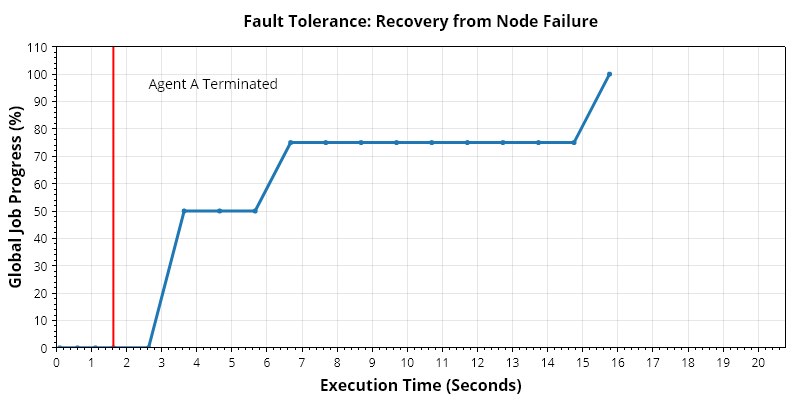
\includegraphics[width=0.8\textwidth]{obrazky-figures/FaultTolerance_Recovery.png}
\caption{A plot visualizing the recovery from a sudden node failure. The red line marks the exact moment Agent A was terminated. After the 6 seconds of missed heartbeats, the \texttt{JobCoordinatorGrain} flagged Agent A as dead, cleanly removed it from the active registry, and re-queued the lost work chunk. Agent B, executing its standby polling loop, detected the reinstated workload, acquired the chunk, and processed it. By successfully achieving 100\% keyspace coverage despite the hardware failure, the result of this test indicates that the system's reliance on telemetry-based leases and at-least-once message delivery ensures data integrity, and eliminates the need for manual administrative intervention.}
\label{fig:fault-tolerance}
\end{figure}

\section{Physical GPU Laboratory Deployment}
\label{sec:gpu_tests}

The physical experiments were performed during a full-day measurement session in the C304 Cisco computer lab at the Faculty of Information Technology, Brno University of Technology. The deployed cluster consisted of 12 laboratory computers with identical hardware:
\begin{itemize}
    \item \textbf{CPU}: AMD Ryzen 5 PRO 5650G
    \item \textbf{RAM}: 64 GB
    \item \textbf{GPU}: NVIDIA GTX 1050 Ti (VRAM: 4 GB)
    %\item \textbf{Operating System}: Microsoft Windows 11
\end{itemize}

The Manager and Coordinator nodes were deployed on a single computer in the LAN with the 10.10.10.118 IP address. The Agent nodes were distributed across the 12 workstations. Real-run artifacts were exported from the DPCS.Blazor web interface as \textit{HTML} snapshots of the Job Details page and \verb|work-units.json| files that contain all detailed metrics about Work Units (chunks) processed by Agents during job execution. The generation of these files is handled by the reporting pipeline displayed by the Attack Report Razor component (as explained in Section \ref{sec:shared_components}). The resulting artifacts are discussed in this chapter alongside the exported lifecycle and telemetry charts.

There were multiple experiments run in total, 3 of which were selected to be presented in the following sections. These experiments tested the capabilities of the system under different scenarios of Mask and Dictionary attack jobs with fast \textbf{MD5} (hash type 0) and slow \textbf{bcrypt} (hash type 3200) hashes, along with varying masks and wordlists. Even though preparations were made to run the Combinator, Hybrid, and Association attack experiment variations, due to time restrictions, only the performance of the base Mask and Dictionary attack modes was thoroughly tested in the end.

\subsection{Synthetic Hash Dataset Generation}

The run experiments use a series of synthetic datasets, which were generated by the utility project \verb|DPCS.HashGenerator|. The main goal of this tool is to prepare repeatable input files for controlled experiments across different Hashcat attack modes.

The generator takes one directory with source wordlists (primarily \verb|rockyou.txt|\footnote{https://weakpass.com/wordlists/rockyou.txt}), an output directory, a target sample count, selected hash types (MD5 and/or bcrypt), a bcrypt work factor, and a parallel thread count. For each scenario, it first creates plaintext candidate samples, then hashes them in parallel, and finally writes three output artifacts: a \verb|.txt| file with hashes only (direct Hashcat input), a \verb|.truth.csv| file with hash-to-plaintext mapping for validation, and a \verb|_manifest.json| file describing attack mode parameters to input in the Blazor web UI.

The plaintext generation step follows the intended attack type. Dictionary scenarios use reservoir sampling over input wordlists. Rule-based scenarios apply simple transformations (for example, capitalization, suffix/prefix additions, or character substitutions). Mask scenarios create candidates from mask tokens and optional custom character sets, including an increment mode where mask length varies within a configured range. Combinator and hybrid scenarios combine sampled wordlist entries with mask-generated fragments according to the selected mode.

After plaintext generation, each candidate is hashed using MD5 (hash mode 0) or bcrypt (hash mode 3200). Hashing is parallelized with \verb|Parallel.ForEach| and a configurable degree of parallelism to reduce dataset preparation time.



\section{Scenario 1: Mask Attack with a Single Mask}

The test dataset for this scenario was generated with a simple mask \verb|?l?l?l?l?l?l| (meaning all combinations of 6-character-long lowercase characters), resulting in a total keyspace of 456,976 password candidates. This scenario was run for both MD5 and bcrypt hashing algorithms. The experiment demonstrated how the Speed-Security paradox, as explained in Section \ref{speed-sec-paradox}, can influence the size of scheduled chunks and the need to set them dynamically on the fly. For a mask of such a small size, the first (MD5) run finished on just a single node in \textbf{2.46 seconds}, and the second (bcrypt) took \textbf{1 hour, 5 minutes, and 15 seconds}.

\begin{table}[H]
    \centering
    \caption{Measured Agent metrics for the MD5 variant of Scenario 1. With a reported hashrate of 2.6 GH/s, the keyspace of 456,976 candidates is too small to justify distribution across multiple Agent nodes. This confirms that the implemented dynamic scheduling logic does not waste compute power on unnecessarily small static chunks.}
    \label{tab:scenario1_md5_md5}
    \footnotesize
    \begin{tabularx}{\textwidth}{|l|l|l|l|l|}
        \hline
         \textbf{Agent PID} & \textbf{Keyspace Coverage} & \textbf{Coverage Share} & \textbf{Total WU} & \textbf{Mean Duration} \\ \hline
         \multirow{3}{*}{10.10.10.110:38039/\$1} & 456,976 & 100.00 \% & 1 & 2.46 s \\ \cline{2-5}
          & \multicolumn{2}{l|}{\textbf{Avg. Hashrate}} & \textbf{Avg. Util.} & \textbf{Avg. Temp.} \\ \cline{2-5}
         &  \multicolumn{2}{l|}{2,600,890,033 H/s} & 89 \% & 56 °C \\ \hline
    \end{tabularx}
\end{table}

The second run with the bcrypt hashes properly distributed the keyspace across the whole cluster of 12 laboratory computers. Due to an implementation limitation of a chunk range minimum of 1,000, the Work Units averaged a longer completion time of about 201.19 seconds and varied hashrates from about 450 to 2,905 H/s. However, observed GPU utilization remained at about 98 to 99\% with small dips when loading the next chunk assignment and starting a new Hashcat process. Temperatures also remained stable, ranging from 55 to 60 °C for all Agent nodes.

\begin{table}[H]
    \centering
    \caption{Measured Work Unit metrics of the Agents participating in the bcrypt variant of Scenario 1. The distribution is fairly even, and the timing differences mainly reflect when each Agent joins the job and when it completes its current work chunk.}
    \label{tab:scenario1_bcrypt_work_units}
    \footnotesize
    \begin{tabular}{|l|l|l|l|l|}
        \hline
         \textbf{Agent PID} & \textbf{Keyspace Coverage} & \textbf{Coverage Share} & \textbf{Total WU} & \textbf{Mean Duration} \\ \hline
         10.10.10.101:3948/\$1 & 38,976 & 8.5 \% & 39 & 198.21 s \\ \hline
         10.10.10.103:9172/\$1 & 38,000 & 8.3 \% & 38 & 203.06 s \\ \hline
         10.10.10.109:19992/\$1 & 38,000 & 8.3 \% & 38 & 201.70 s \\ \hline
         10.10.10.110:38039/\$1 & 39,000 & 8.5 \% & 39 & 196.60 s \\ \hline
         10.10.10.111:47883/\$1 & 38,000 & 8.3 \% & 38 & 203.32 s \\ \hline
         10.10.10.112:37796/\$1 & 37,000 & 8.1 \% & 37 & 205.13 s \\ \hline
         10.10.10.113:37048/\$1 & 38,000 & 8.3 \% & 38 & 203.14 s \\ \hline
         10.10.10.114:46447/\$1 & 39,000 & 8.5 \% & 39 & 195.22 s \\ \hline
         10.10.10.115:16423/\$1 & 38,000 & 8.3 \% & 38 & 201.25 s \\ \hline
         10.10.10.116:10682/\$1 & 38,000 & 8.3 \% & 38 & 200.05 s \\ \hline
         10.10.10.117:12661/\$1 & 38,000 & 8.3 \% & 38 & 203.24 s \\ \hline
         10.10.10.118:48505/\$1 & 37,000 & 8.1 \% & 37 & 203.91 s \\ \hline
        \textbf{Cluster} & 456,976 & 100.0 \% & 457 & 208.11 s \\ \hline
    \end{tabular}
\end{table}

\begin{table}[H]
    \centering
    \caption{Measured GPU metrics of all Agents participating in the bcrypt variant of Scenario 1. The results are broadly consistent because all nodes used the same NVIDIA GeForce 1050 Ti hardware.}
    \label{tab:scenario1_bcrypt_gpu}
    \footnotesize
    \begin{tabular}{|l|l|l|l|l|}
        \hline
         \textbf{Agent PID} & \textbf{Average Hashrate} & \textbf{Average GPU Util.} & \textbf{Average GPU Temp.} \\ \hline
         10.10.10.101:3948/\$1 & 1,729 H/s & 98 \% & 57 °C \\ \hline
         10.10.10.103:9172/\$1 & 1,719 H/s & 94 \% & 56 °C \\ \hline
         10.10.10.109:19992/\$1 & 1,718 H/s & 98 \% & 56 °C \\ \hline
         10.10.10.110:38039/\$1 & 1,725 H/s & 98 \% & 58 °C \\ \hline
         10.10.10.111:47883/\$1 & 1,719 H/s & 99 \% & 57 °C \\ \hline
         10.10.10.112:37796/\$1 & 1,717 H/s & 99 \% & 56 °C \\ \hline
         10.10.10.113:37048/\$1 & 1,719 H/s & 99 \% & 57 °C \\ \hline
         10.10.10.114:46447/\$1 & 1,727 H/s & 99 \% & 57 °C \\ \hline
         10.10.10.115:16423/\$1 & 1,722 H/s & 99 \% & 58 °C \\ \hline
         10.10.10.116:10682/\$1 & 1,723 H/s & 99 \% & 56 °C \\ \hline
         10.10.10.117:12661/\$1 & 1,718 H/s & 98 \% & 57 °C \\ \hline
         10.10.10.118:48505/\$1 & 1,715 H/s & 93 \% & 57 °C \\ \hline
    \end{tabular}
\end{table}

\begin{figure}[H]
\centering
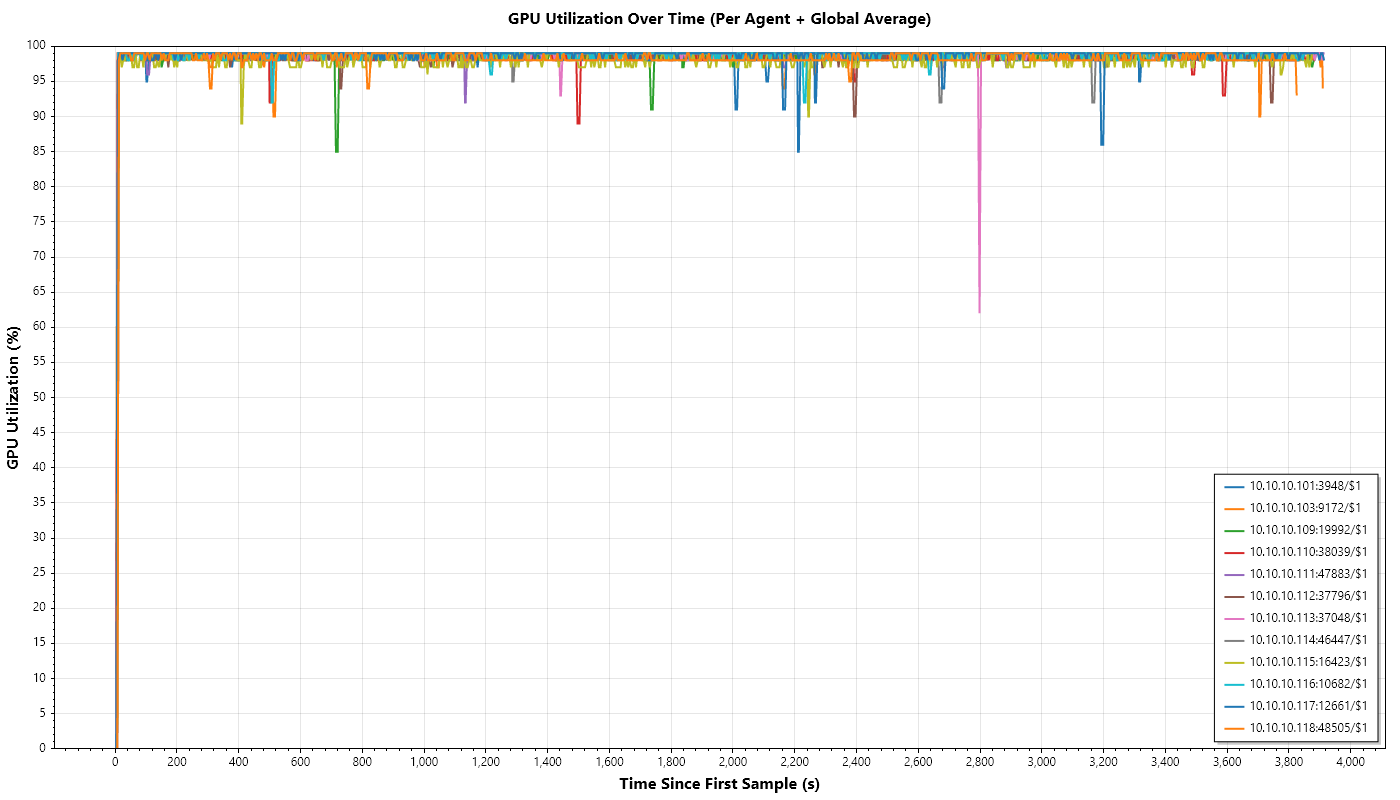
\includegraphics[width=\textwidth]{obrazky-figures/exp1/gpu-usage.png}
\caption{Chart of the observed GPU usage per Agent over time. All Agents remained close to full utilization throughout the run. Small dips occurred briefly when an Agent submitted the result of its assigned chunk and started the next Hashcat process.}
\label{fig:exp1-gpu-usage}
\end{figure}

\begin{figure}[H]
\centering
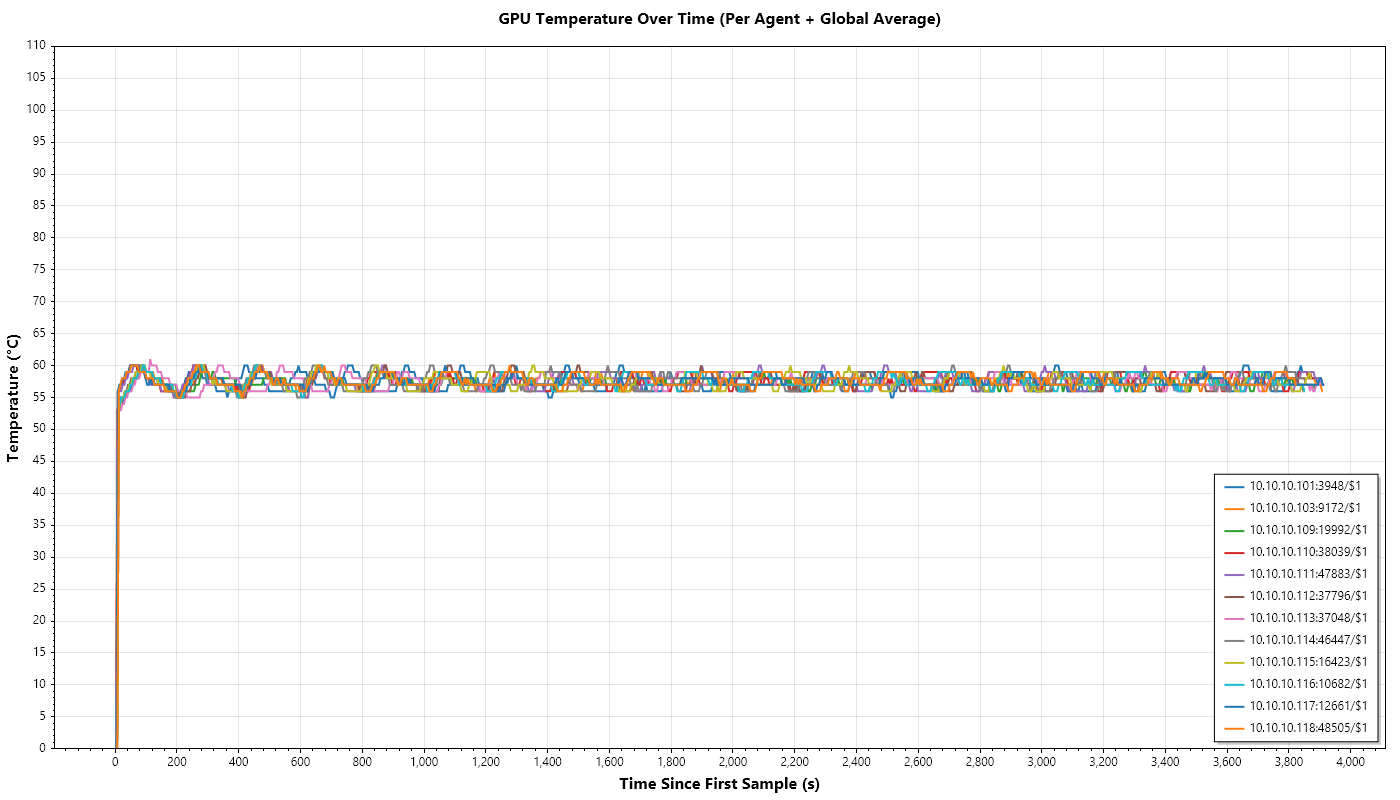
\includegraphics[width=\textwidth]{obrazky-figures/exp1/gpu-temp.png}
\caption{Chart of the observed GPU temperature per Agent over time. Temperatures increased slightly over time, but remained stable overall within the 55 to 60 °C range.}
\label{fig:exp1-gpu-temp}
\end{figure}

\begin{figure}[H]
\centering
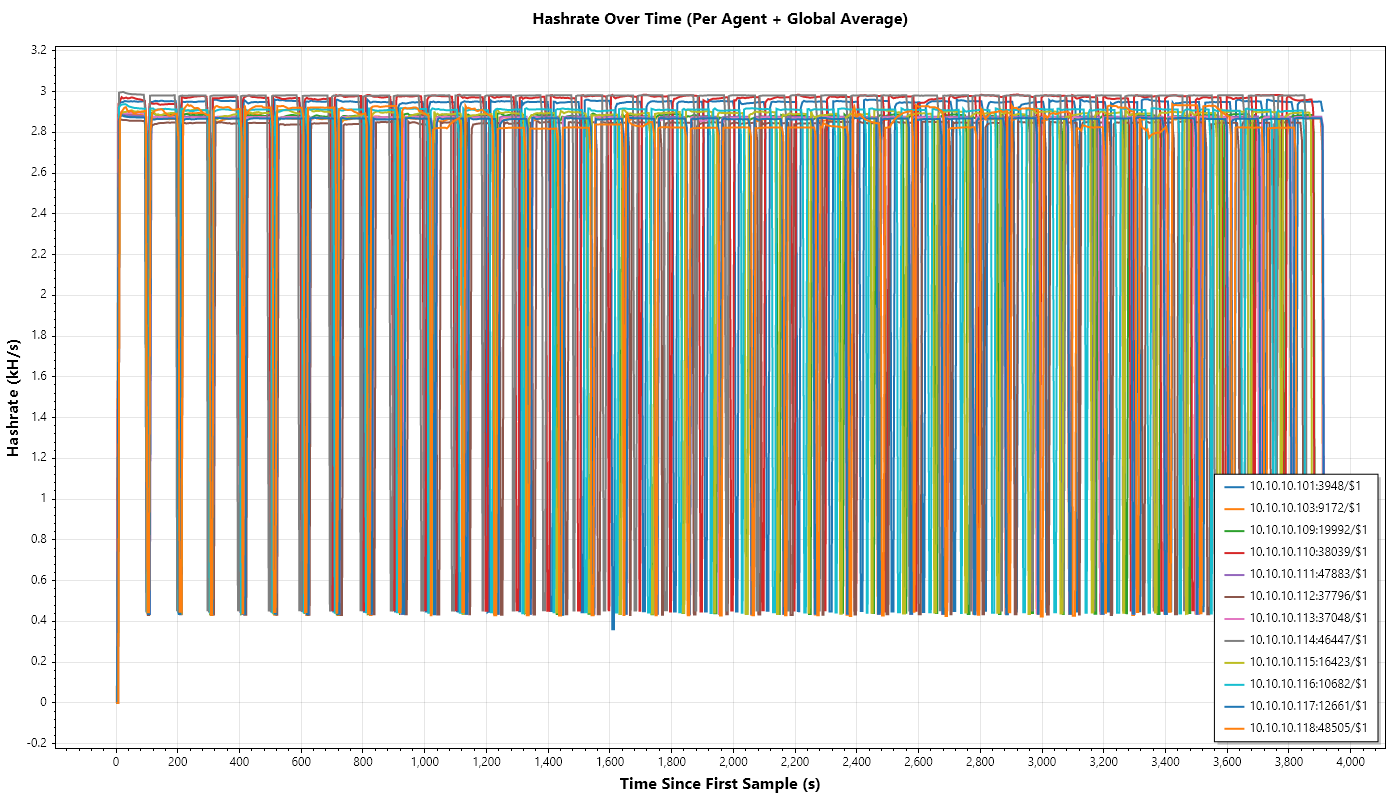
\includegraphics[width=\textwidth]{obrazky-figures/exp1/gpu-hashrate.png}
\caption{Chart of the observed GPU hashrate per Agent over time. The hashrate varied at the start and end of processed chunks across Agents, ranging from about 450 to 3,000 H/s, which is consistent with the slow bcrypt algorithm.}
\label{fig:exp1-gpu-hashrate}
\end{figure}

\begin{figure}[H]
\centering
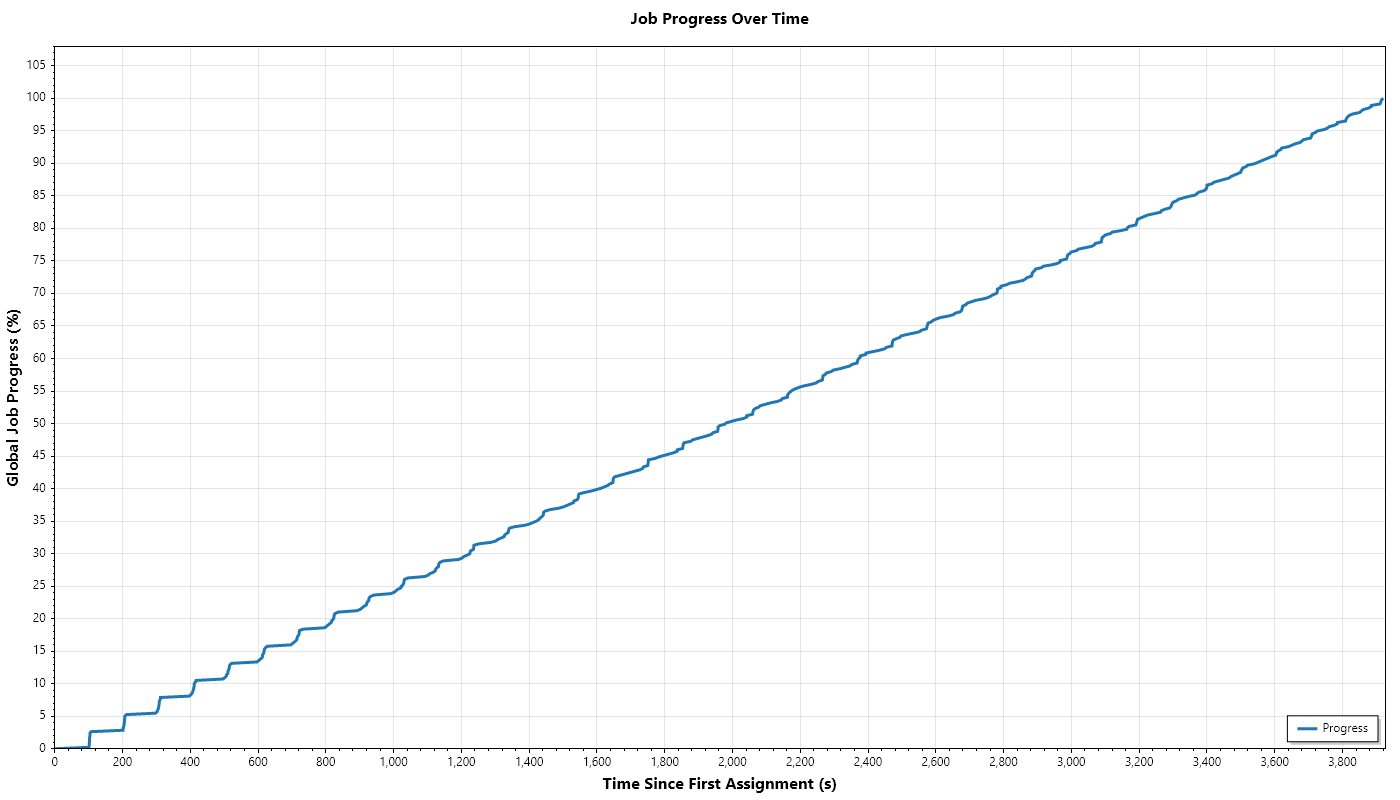
\includegraphics[width=\textwidth]{obrazky-figures/exp1/job-progress.png}
\caption{Chart of the observed overall job progression percentage over time. At the start, Agents began and completed their first chunks at similar times, resulting in sudden jumps in the progress percentage. Later chunks were assigned and acknowledged at different times, and the overall progress increased more smoothly and linearly.}
\label{fig:exp1-job-progress}
\end{figure}

\section{Scenario 2: Mask Attack with Iteration Mode / Multiple Masks}

This scenario evaluates a mask attack where the search domain is expanded through multiple masks of increasing complexity. The \textbf{Iteration Mode} option in the mask attack with mask \verb|?l?l?l?l?l?l?l?l?d?d?d|, minimum length value set to \textbf{8} and maximum length set to \textbf{11} generates a total of 4 masks: 8 lowercase characters, then 8 lowercase + 1 digit, then +2 digits, and finally +3 digits. The evaluated run used MD5 hashes (hash mode 0) with the same Coordinator target of 30 seconds per chunk.

According to the exported report for this scenario, the system searched through the combined keyspace of \textbf{1,512,341,703 candidates} out of the total \textbf{13,200,208,736 possible candidates} because a matching recovered password was found for all submitted hashes, so the job execution ended early.

\begin{table}[hbt]
    \centering
    \caption{Per-mask overview of the total keyspace size and the number of Work Units distributed across Agents.}
    \label{tab:scenario2_mask_overview}
    \footnotesize
    \begin{tabular}{|l|l|l|l|l|}
        \hline
         \textbf{Mask} & \textbf{Total Keyspace} & \textbf{Total run Work Units} \\ \hline
         \verb|?l?l?l?l?l?l?l?l| & 11,881,376 & 3 \\ \hline
         \verb|?l?l?l?l?l?l?l?l?d| & 118,813,760 & 26 \\ \hline
         \verb|?l?l?l?l?l?l?l?l?d?d| & 1,188,137,600 & 252 \\ \hline
         \verb|?l?l?l?l?l?l?l?l?d?d?d| & 11,881,376,000 & 41 \\ \hline
         \textbf{Combined} & 13,200,208,736 & 322 \\ \hline
    \end{tabular}
\end{table}

The run finished with a total of \textbf{322 Work Unit attempts}. The whole job took \textbf{11 minutes and 32 seconds}, with all 12 Agents participating in completing it. The key observation is that iteration-mode masks are computationally much larger than the single-mask baseline from Scenario 1, but the dynamic scheduler still kept chunk durations near the configured target order of magnitude, with a mean duration of about \textbf{49.53 s} and no timed-out work units.

\begin{table}[hbt]
    \centering
    \caption{Measured Work Unit metrics of Agents participating in the iterative mask run of Scenario 2. The distribution remained balanced across the full cluster despite the much larger combined keyspace.}
    \label{tab:scenario2_work_units}
    \footnotesize
    \begin{tabular}{|l|l|l|l|l|}
        \hline
         \textbf{Agent PID} & \textbf{Keyspace Coverage} & \textbf{Coverage Share} & \textbf{Total WU} & \textbf{Mean Duration} \\ \hline
         10.10.10.101:3948/\$1 & 124,722,650 & 8.2 \% & 26 & 50.62 s \\ \hline
         10.10.10.103:9172/\$1 & 126,460,440 & 8.4 \% & 27 & 50.09 s \\ \hline
         10.10.10.109:19992/\$1 & 122,138,952 & 8.1 \% & 26 & 50.40 s \\ \hline
         10.10.10.110:38039/\$1 & 127,981,053 & 8.5 \% & 27 & 48.73 s \\ \hline
         10.10.10.111:47883/\$1 & 130,174,632 & 8.6 \% & 28 & 48.02 s \\ \hline
         10.10.10.112:37796/\$1 & 124,946,496 & 8.3 \% & 27 & 49.69 s \\ \hline
         10.10.10.113:37048/\$1 & 123,197,958 & 8.1 \% & 26 & 50.79 s \\ \hline
         10.10.10.114:46447/\$1 & 129,848,125 & 8.6 \% & 28 & 46.67 s \\ \hline
         10.10.10.115:16423/\$1 & 123,997,181 & 8.2 \% & 27 & 48.24 s \\ \hline
         10.10.10.116:10682/\$1 & 129,436,029 & 8.6 \% & 27 & 49.97 s \\ \hline
         10.10.10.117:12661/\$1 & 124,278,347 & 8.2 \% & 27 & 49.99 s \\ \hline
         10.10.10.118:48505/\$1 & 125,159,840 & 8.3 \% & 26 & 51.52 s \\ \hline
         \textbf{Cluster} & 1,512,341,703 & 100.0 \% & 322 & 49.53 s \\ \hline
    \end{tabular}
\end{table}

\begin{table}[hbt]
    \centering
    \caption{Measured GPU metrics of all Agents, participating in the job, running the iterative mask version of Scenario 2. All nodes stayed close to full utilization and reported similar  thermals, which confirms that this scenario remained predominantly compute-bound rather than transfer-bound.}
    \label{tab:scenario2_gpu}
    \footnotesize
    \begin{tabular}{|l|l|l|l|}
        \hline
         \textbf{Agent PID} & \textbf{Average Hashrate} & \textbf{Average GPU Util.} & \textbf{Average GPU Temp.} \\ \hline
         10.10.10.101:3948/\$1 & 3,737,131,323 H/s & 99 \% & 74 °C \\ \hline
         10.10.10.103:9172/\$1 & 3,587,653,484 H/s & 99 \% & 75 °C \\ \hline
         10.10.10.109:19992/\$1 & 3,586,104,383 H/s & 99 \% & 77 °C \\ \hline
         10.10.10.110:38039/\$1 & 3,791,710,637 H/s & 99 \% & 77 °C \\ \hline
         10.10.10.111:47883/\$1 & 3,587,669,206 H/s & 99 \% & 75 °C \\ \hline
         10.10.10.112:37796/\$1 & 3,587,144,834 H/s & 99 \% & 76 °C \\ \hline
         10.10.10.113:37048/\$1 & 3,736,547,565 H/s & 99 \% & 76 °C \\ \hline
         10.10.10.114:46447/\$1 & 3,734,380,753 H/s & 99 \% & 74 °C \\ \hline
         10.10.10.115:16423/\$1 & 3,605,894,945 H/s & 98 \% & 75 °C \\ \hline
         10.10.10.116:10682/\$1 & 3,626,112,668 H/s & 99 \% & 75 °C \\ \hline
         10.10.10.117:12661/\$1 & 3,719,874,994 H/s & 98 \% & 79 °C \\ \hline
         10.10.10.118:48505/\$1 & 3,558,170,808 H/s & 98 \% & 75 °C \\ \hline
    \end{tabular}
\end{table}

\begin{figure}[H]
\centering

\includegraphics[width=\textwidth]{obrazky-figures/exp2/gpu-usage.png}
\caption{Scenario 2 GPU utilization over time across participating Agents. Overall, they remained close to full utilization throughout the run, with only brief dips no lower than 85 \%.}
\label{fig:exp2-gpu-usage}
\end{figure}

\begin{figure}[H]
\centering

\includegraphics[width=\textwidth]{obrazky-figures/exp2/gpu-temp.png}
\caption{Scenario 2 GPU temperature evolution during iterative mask processing. During this run, temperatures increased compared with Scenario 1, but remained consistent between 65 and 75 °C.}
\label{fig:exp2-gpu-temp}
\end{figure}

\begin{figure}[H]
\centering

\includegraphics[width=\textwidth]{obrazky-figures/exp2/gpu-hashrate.png}
\caption{Scenario 2 per-Agent hashrate profile. Compared with Scenario 1, which used a simpler mask and the bcrypt algorithm, the hashrate remained more stable over time, ranging from about 3.5 to 3.9 GH/s.}
\label{fig:exp2-gpu-hashrate}
\end{figure}

\begin{figure}[H]
\centering

\includegraphics[width=\textwidth]{obrazky-figures/exp2/job-progress.png}
\caption{Scenario 2 overall job progress over time. The job progressed mostly steadily and linearly until the end, when all submitted hashes had been matched. This also demonstrates how the system exits early and does not waste computational resources once all relevant work has been completed.}
\label{fig:exp2-job-progress}
\end{figure}

\section{Scenario 3: Dictionary Attack with rockyou.txt}

Scenario 3 was executed in two variants over the well-known \verb|rockyou.txt|\footnote{https://weakpass.com/wordlists/rockyou.txt} wordlist without rules: a fast-hash MD5 run and a slow-hash bcrypt run. This pair directly demonstrates the runtime impact of the selected hash algorithm while keeping the dictionary source constant.

The MD5 variant was completed in a single chunk by a single participant because the \textbf{133.4 MiB} size of the \verb|rockyou.txt| wordlist was not sufficient to justify distribution across multiple Agents in this configuration. The run finished in \textbf{5.20 s}. By contrast, the bcrypt variant kept \textbf{12 participating Agents} occupied for \textbf{1 hour, 11 minutes, and 48 seconds} and recorded \textbf{178 total work-unit attempts}. This is consistent with the speed-security paradox discussed in Chapter 2: for the same dictionary coverage, bcrypt dramatically increases the compute cost per candidate and, therefore, the total runtime.

\begin{table}[hbt]
    \centering
    \caption{Measured Work Unit and GPU metrics for the MD5 variant of Scenario 3. As in Scenario 1, the workload remained on a single Agent because the input size was too small relative to the measured throughput to justify further splitting.}
    \label{tab:scenario3_md5}
    \footnotesize
    \hline
    \begin{tabularx}{\textwidth}{|l|l|l|l|l|}
         \textbf{Agent PID} & \multicolumn{1}{l|}{\textbf{Keyspace Coverage}} & \textbf{Coverage Share} & \textbf{Total WU} & \textbf{Mean Duration} \\ \hline
         \multirow{3}{*}{10.10.10.113:37048/\$1} & \multicolumn{1}{l|}{133.4 MiB} & 100.00 \% & 1 & 5.20 s \\ \cline{2-5}
         & \multicolumn{2}{l|}{\textbf{Avg. Hashrate}} & \textbf{Avg. Util.} & \textbf{Avg. Temp.} \\ \cline{2-5}
         & \multicolumn{2}{l|}{18,500,644 H/s} & 39 \% & 49 °C \\ \hline
    \end{tabularx}
\end{table}

The bcrypt variant distributed the same \textbf{133.4 MiB} dictionary across the full cluster and kept Work Unit durations clustered around the \textbf{539.05 s} mean. Per-node throughput ranged from about \textbf{2,784 H/s} to \textbf{2,955 H/s}, while observed GPU utilization stayed mostly between \textbf{97 \%} and \textbf{99 \%}. This behavior closely matches the long-running, compute-bound profile expected from bcrypt.

\begin{table}[H]
    \centering
    \caption{Measured Work Unit metrics of Agents participating in the job running the bcrypt version of Scenario 3. The work distribution was close to even, with only minor differences caused by the exact moment at which each Agent joined the job and received its first long-running assignment. It is also worth noting that, although the Agent \textit{10.10.10.118:48505/\$1} ran on the same machine as the Coordinator node, it received essentially the same total number of Work Units and the same amount of wordlist data as the other nodes.}
    \label{tab:scenario3_bcrypt_work_units}
    \footnotesize
    \begin{tabular}{|l|l|l|l|l|}
        \hline
         \textbf{Agent PID} & \textbf{Keyspace Coverage} & \textbf{Coverage Share} & \textbf{Total WU} & \textbf{Mean Duration} \\ \hline
         10.10.10.101:3948/\$1 & 11.1 MiB & 8.3 \% & 15 & 542.89 s \\ \hline
         10.10.10.103:9172/\$1 & 10.3 MiB & 7.7 \% & 14 & 557.00 s \\ \hline
         10.10.10.109:19992/\$1 & 10.3 MiB & 7.7 \% & 14 & 553.68 s \\ \hline
         10.10.10.110:38039/\$1 & 11.9 MiB & 8.9 \% & 16 & 511.51 s \\ \hline
         10.10.10.111:47883/\$1 & 11.2 MiB & 8.4 \% & 15 & 537.09 s \\ \hline
         10.10.10.112:37796/\$1 & 10.5 MiB & 7.9 \% & 14 & 551.89 s \\ \hline
         10.10.10.113:37048/\$1 & 10.6 MiB & 7.9 \% & 14 & 558.21 s \\ \hline
         10.10.10.114:46447/\$1 & 14.3 MiB & 10.7 \% & 17 & 471.30 s \\ \hline
         10.10.10.115:16423/\$1 & 11.0 MiB & 8.2 \% & 15 & 551.72 s \\ \hline
         10.10.10.116:10682/\$1 & 10.8 MiB & 8.1 \% & 15 & 538.67 s \\ \hline
         10.10.10.117:12661/\$1 & 10.5 MiB & 7.9 \% & 14 & 558.11 s \\ \hline
         10.10.10.118:48505/\$1 & 11.1 MiB & 8.3 \% & 15 & 553.25 s \\ \hline
    \end{tabular}
\end{table}

\begin{table}[H]
    \centering
    \caption{Measured GPU metrics of all Agents, participating in the job, running the bcrypt version of Scenario 3.}
    \label{tab:scenario3_bcrypt_gpu}
    \footnotesize
    \begin{tabular}{|l|l|l|l|}
        \hline
         \textbf{Agent PID} & \textbf{Average Hashrate} & \textbf{Average GPU Util.} & \textbf{Average GPU Temp.} \\ \hline
         10.10.10.101:3948/\$1 & 2,936 H/s & 98 \% & 59 °C \\ \hline
         10.10.10.103:9172/\$1 & 2,807 H/s & 98 \% & 57 °C \\ \hline
         10.10.10.109:19992/\$1 & 2,823 H/s & 98 \% & 57 °C \\ \hline
         10.10.10.110:38039/\$1 & 2,955 H/s & 99 \% & 58 °C \\ \hline
         10.10.10.111:47883/\$1 & 2,820 H/s & 99 \% & 59 °C \\ \hline
         10.10.10.112:37796/\$1 & 2,784 H/s & 97 \% & 57 °C \\ \hline
         10.10.10.113:37048/\$1 & 2,810 H/s & 99 \% & 57 °C \\ \hline
         10.10.10.114:46447/\$1 & 2,918 H/s & 98 \% & 59 °C \\ \hline
         10.10.10.115:16423/\$1 & 2,882 H/s & 97 \% & 58 °C \\ \hline
         10.10.10.116:10682/\$1 & 2,829 H/s & 98 \% & 57 °C \\ \hline
         10.10.10.117:12661/\$1 & 2,808 H/s & 91 \% & 57 °C \\ \hline
         10.10.10.118:48505/\$1 & 2,844 H/s & 98 \% & 58 °C \\ \hline
    \end{tabular}
\end{table}


\begin{figure}[H]
\centering

\includegraphics[width=\textwidth]{obrazky-figures/exp3/gpu-usage.png}
\caption{Scenario 3 (bcrypt) GPU utilization over time. All Agents remained close to full utilization throughout the run, indicating that the tasks were more compute-bound than network-bound. The prefetching logic therefore worked as expected: while Hashcat processed the currently assigned wordlist chunk, the next chunk was downloaded in the background quickly enough to be processed immediately once the previous Hashcat process had finished.}
\label{fig:exp3-bcrypt-gpu-usage}
\end{figure}

\begin{figure}[H]
\centering

\includegraphics[width=\textwidth]{obrazky-figures/exp3/gpu-temp.png}
\caption{Scenario 3 (bcrypt) GPU temperature profile. The temperatures remained stable, ranging from 55 to 60 °C.}
\label{fig:exp3-bcrypt-gpu-temp}
\end{figure}

\begin{figure}[H]
\centering

\includegraphics[width=\textwidth]{obrazky-figures/exp3/gpu-hashrate.png}
\caption{Scenario 3 (bcrypt) hashrate profile. The overall hashrate remained stable over time, ranging from about 2.8 to 3 kH/s, which is consistent with the results observed in Scenario 2.}
\label{fig:exp3-bcrypt-gpu-hashrate}
\end{figure}

\begin{figure}[H]
\centering

\includegraphics[width=\textwidth]{obrazky-figures/exp3/job-progress.png}
\caption{Scenario 3 (bcrypt) overall progress over time. Similar to Scenario 1, the global job-progress percentage exhibited sudden jumps as Agents reported their work results at similar times. This behavior remained consistent until the end.}
\label{fig:exp3-bcrypt-job-progress}
\end{figure}

\begin{comment}
\section{Scenario 4: Dictionary Attack with weakpass\_4.policy.txt}

Scenario 4 used the \verb|weakpass_4.policy.txt|\footnote{https://weakpass.com/wordlists/weakpass\_4.policy.txt} wordlist with MD5 hashes to test it with a substantially larger dictionary volume of \textbf{3.5 GiB} than Scenario 3, which used the smaller rockyou.txt wordlist.

Even with multi-gigabyte input coverage, the run completed without retries or timeouts, finished all \textbf{20 Work Units}, and reached completion in only \textbf{33.72 seconds}. The measured mean Work Unit duration was \textbf{17.64 s}. This result supports the practical viability of the HTTP byte-range distribution model under fast-hash conditions, where data movement and orchestration overhead become more visible than the cryptographic primitive itself. However, better results could possibly be observed with even larger dictionaries or by using rules to expand the wordlist candidate count, which could run longer. The same can be said for using bcrypt as the hashing algorithm (like the previous scenarios); however, based on the run times previously seen with the smaller rockyou.txt wordlist, which job ran for over 1 hour, this scenario is expected to run for multiple hours. This was not feasible to measure during the single-day session in the C304 lab.

\begin{table}[H]
    \centering
    \caption{Measured Work Unit metrics of Agents participating in the job running the MD5 weakpass dictionary version of Scenario 4. The work was shared fairly evenly, although the full job was divided into only a small number of relatively large byte ranges, so the share per Agent varied more than in the longer-running bcrypt experiments. The workload was still drained quickly by the cluster. It is also worth noting that some Agents had mean durations close to the expected 30-second target, while lower values were caused by the Coordinator notifying Agents to cancel unfinished work once all passwords had already been found and the Agent was still in the middle of downloading a wordlist chunk or processing it with Hashcat.}
    \label{tab:scenario4_work_units}
    \footnotesize
    \begin{tabular}{|l|l|l|l|l|}
        \hline
         \textbf{Agent PID} & \textbf{Keyspace Coverage} & \textbf{Coverage Share} & \textbf{Total WU} & \textbf{Mean Duration} \\ \hline
         10.10.10.101:3948/\$1 & 248.0 MiB & 7.0 \% & 1 & 29.99 s \\ \hline
         10.10.10.103:9172/\$1 & 191.4 MiB & 5.4 \% & 1 & 32.94 s \\ \hline
         10.10.10.109:19992/\$1 & 230.4 MiB & 6.5 \% & 1 & 33.02 s \\ \hline
         10.10.10.110:38039/\$1 & 312.4 MiB & 8.8 \% & 2 & 14.74 s \\ \hline
         10.10.10.111:47883/\$1 & 129.8 MiB & 3.7 \% & 1 & 21.81 s \\ \hline
         10.10.10.112:37796/\$1 & 331.1 MiB & 9.3 \% & 2 & 17.06 s \\ \hline
         10.10.10.113:37048/\$1 & 216.2 MiB & 6.1 \% & 1 & 23.56 s \\ \hline
         10.10.10.114:46447/\$1 & 201.4 MiB & 5.7 \% & 1 & 29.49 s \\ \hline
         10.10.10.115:16423/\$1 & 318.3 MiB & 9.0 \% & 2 & 14.79 s \\ \hline
         10.10.10.116:10682/\$1 & 397.6 MiB & 11.2 \% & 2 & 10.86 s \\ \hline
         10.10.10.117:12661/\$1 & 281.1 MiB & 7.9 \% & 2 & 13.56 s \\ \hline
         10.10.10.118:48505/\$1 & 695.0 MiB & 19.6 \% & 4 & 10.00 s \\ \hline
         \textbf{Cluster} & 3.5 GiB & 100.0 \% & 20 & 17.64 s \\ \hline
    \end{tabular}
\end{table}

\begin{table}[H]
    \centering
    \caption{Measured GPU metrics of all Agents, participating in the job, running the MD5 weakpass dictionary version of Scenario 4. Compared with the slower bcrypt workloads, GPU utilization is much lower here because each chunk finishes quickly and orchestration overhead becomes visible between assignments.}
    \label{tab:scenario4_gpu}
    \footnotesize
    \begin{tabular}{|l|l|l|l|}
        \hline
         \textbf{Agent PID} & \textbf{Average Hashrate} & \textbf{Average GPU Util.} & \textbf{Average GPU Temp.} \\ \hline
         10.10.10.101:3948/\$1 & 18,618,568 H/s & 40 \% & 51 °C \\ \hline
         10.10.10.103:9172/\$1 & 18,803,037 H/s & 38 \% & 50 °C \\ \hline
         10.10.10.109:19992/\$1 & 18,227,717 H/s & 35 \% & 51 °C \\ \hline
         10.10.10.110:38039/\$1 & 18,950,240 H/s & 39 \% & 54 °C \\ \hline
         10.10.10.111:47883/\$1 & 19,193,919 H/s & 39 \% & 52 °C \\ \hline
         10.10.10.112:37796/\$1 & 18,521,425 H/s & 45 \% & 51 °C \\ \hline
         10.10.10.113:37048/\$1 & 19,030,517 H/s & 39 \% & 49 °C \\ \hline
         10.10.10.114:46447/\$1 & 18,881,323 H/s & 39 \% & 51 °C \\ \hline
         10.10.10.115:16423/\$1 & 19,925,093 H/s & 38 \% & 56 °C \\ \hline
         10.10.10.116:10682/\$1 & 19,203,624 H/s & 36 \% & 53 °C \\ \hline
         10.10.10.117:12661/\$1 & 18,617,325 H/s & 36 \% & 53 °C \\ \hline
         10.10.10.118:48505/\$1 & 17,956,488 H/s & 35 \% & 55 °C \\ \hline
    \end{tabular}
\end{table}

\begin{figure}[H]
\centering

\includegraphics[width=\textwidth]{obrazky-figures/exp4/gpu-usage.png}
\caption{Scenario 4 GPU utilization over time. This shows that even the 3.5 GiB wordlist was not large enough for a cluster of 12 Agents, resulting in a short overall runtime but poor GPU utilization, because the Work Units finished quickly or were cancelled by the Coordinator once all passwords for the submitted hashes had been found. It is also apparent that some Agents stopped reporting once their work had finished, while other chunks had already been assigned to different Agents that started later.}
\label{fig:exp4-gpu-usage}
\end{figure}

\begin{figure}[H]
\centering

\includegraphics[width=\textwidth]{obrazky-figures/exp4/gpu-temp.png}
\caption{Scenario 4 GPU temperature profile. During this short run, with lower GPU utilization, temperatures remained close to the baseline range of about 50 to 55 °C.}
\label{fig:exp4-gpu-temp}
\end{figure}

\begin{figure}[H]
\centering

\includegraphics[width=\textwidth]{obrazky-figures/exp4/gpu-hashrate.png}
\caption{Scenario 4 hashrate profile. The lower observed GPU utilization is reflected in a lower hashrate than in the other MD5-based scenarios.}
\label{fig:exp4-gpu-hashrate}
\end{figure}

\begin{figure}[H]
\centering

\includegraphics[width=\textwidth]{obrazky-figures/exp4/job-progress.png}
\caption{Scenario 4 overall job progress over time. The chart shows the same pattern of sudden jumps in progress as Agents submitted results in a first wave, followed by a single final chunk that pushed the job to 100 \% completion and triggered cancellation of unfinished work.}
\label{fig:exp4-job-progress}
\end{figure}
\end{comment}

\begin{comment}
    
\section{Scenario 5: Hybrid Attack with rockyou.txt}

Scenario 5 evaluates attack mode 6 (Hybrid Wordlist + Mask) on MD5. The exported Work Unit records show a total keyspace coverage of \textbf{7,410 candidates}, decomposed into \textbf{741 Work Unit attempts}, with \textbf{718 completed attempts (96.9\%)} and no retries or timeouts.

Although the run reached full logical progress, no plaintext from the target set was recovered for this specific configuration of \verb|rockyou.txt| with the tested suffix mask pattern. The JSON timeline shows a total wall-clock duration of \textbf{152.48 s}, while the attack report recorded a mean work-unit duration of \textbf{4.93 s}. The final status is \textbf{Cancelled}, which reflects operational interruption behavior rather than algorithmic failure. It confirms that already completed work is still captured in the generated report artifacts. The last exported telemetry state also marks all Agents as dead, which is why the averaged hashrate and utilization fields in the table below remain at zero, even though the completed work itself was recorded correctly.

\begin{table}[hbt]
    \centering
    \caption{Measured Work Unit metrics of Agents, participating in the job, running the hybrid wordlist-plus-mask version of Scenario 5. The distribution remained almost perfectly even because the scheduler worked with many short work units over a relatively small total keyspace.}
    \label{tab:scenario5_work_units}
    \footnotesize
    \begin{tabular}{|l|l|l|l|l|}
        \hline
         \textbf{Agent PID} & \textbf{Keyspace Coverage} & \textbf{Coverage Share} & \textbf{Total WU} & \textbf{Mean Duration} \\ \hline
         10.10.10.101:3948/\$1 & 610 & 8.2 \% & 61 & 4.95 s \\ \hline
         10.10.10.103:9172/\$1 & 620 & 8.4 \% & 62 & 4.90 s \\ \hline
         10.10.10.109:19992/\$1 & 620 & 8.4 \% & 62 & 4.87 s \\ \hline
         10.10.10.110:38039/\$1 & 620 & 8.4 \% & 62 & 4.90 s \\ \hline
         10.10.10.111:47883/\$1 & 630 & 8.5 \% & 63 & 4.85 s \\ \hline
         10.10.10.112:37796/\$1 & 610 & 8.2 \% & 61 & 4.98 s \\ \hline
         10.10.10.113:37048/\$1 & 620 & 8.4 \% & 62 & 4.87 s \\ \hline
         10.10.10.114:46447/\$1 & 630 & 8.5 \% & 63 & 4.86 s \\ \hline
         10.10.10.115:16423/\$1 & 610 & 8.2 \% & 61 & 4.97 s \\ \hline
         10.10.10.116:10682/\$1 & 620 & 8.4 \% & 62 & 4.91 s \\ \hline
         10.10.10.117:12661/\$1 & 620 & 8.4 \% & 62 & 4.95 s \\ \hline
         10.10.10.118:48505/\$1 & 600 & 8.1 \% & 60 & 5.15 s \\ \hline
    \end{tabular}
\end{table}

\begin{table}[hbt]
    \centering
    \caption{Measured GPU metrics of all Agents, participating in the job, running the hybrid wordlist-plus-mask version of Scenario 5. The zeroed hashrate and utilization values are a consequence of the final exported state after cancellation rather than an indication that the assigned work was never processed.}
    \label{tab:scenario5_gpu}
    \footnotesize
    \begin{tabular}{|l|l|l|l|}
        \hline
         \textbf{Agent PID} & \textbf{Average Hashrate} & \textbf{Average GPU Util.} & \textbf{Average GPU Temp.} \\ \hline
         10.10.10.101:3948/\$1  & 1,130,710 H/s & 96 \% & 62 °C \\ \hline
         10.10.10.103:9172/\$1  & 1,725,327 H/s & 99 \% & 63 °C \\ \hline
         10.10.10.109:19992/\$1 & 1,693,193 H/s & 99 \% & 61 °C \\ \hline
         10.10.10.110:38039/\$1 & 1,117,942 H/s & 99 \% & 61 °C \\ \hline
         10.10.10.111:47883/\$1 & 1,607,717 H/s & 99 \% & 62 °C \\ \hline
         10.10.10.112:37796/\$1 & 1,039,717 H/s & 91 \% & 61 °C \\ \hline
         10.10.10.113:37048/\$1 & 1,723,840 H/s & 99 \% & 62 °C \\ \hline
         10.10.10.114:46447/\$1 & 1,546,790 H/s & 89 \% & 62 °C \\ \hline
         10.10.10.115:16423/\$1 & 1,551,590 H/s & 99 \% & 60 °C \\ \hline
         10.10.10.116:10682/\$1 & 1,114,206 H/s & 89 \% & 61 °C \\ \hline
         10.10.10.117:12661/\$1 & 1,610,824 H/s & 98 \% & 63 °C \\ \hline
         10.10.10.118:48505/\$1 & 1,452,432 H/s & 88 \% & 60 °C \\ \hline
    \end{tabular}
\end{table}

\begin{figure}[H]
\centering

\includegraphics[width=\textwidth]{obrazky-figures/exp5/gpu-usage.png}
\caption{Scenario 5 GPU utilization over time.}
\label{fig:exp5-gpu-usage}
\end{figure}

\begin{figure}[H]
\centering

\includegraphics[width=\textwidth]{obrazky-figures/exp5/gpu-temp.png}
\caption{Scenario 5 GPU temperature profile.}
\label{fig:exp5-gpu-temp}
\end{figure}

\begin{figure}[H]
\centering

\includegraphics[width=\textwidth]{obrazky-figures/exp5/gpu-hashrate.png}
\caption{Scenario 5 hashrate profile (inactive/zero because Agents are marked dead at the end state).}
\label{fig:exp5-gpu-hashrate}
\end{figure}

\begin{figure}[H]
\centering

\includegraphics[width=\textwidth]{obrazky-figures/exp5/job-progress.png}
\caption{Scenario 5 overall progress over time.}
\label{fig:exp5-job-progress}
\end{figure}

\end{comment}

\begin{comment}
\subsection{Executed Scenarios and Aggregate Outcomes}
Table \ref{tab:real-gpu-runs} lists the key runs completed in C304. It combines data from the per-job attack report cards and work-unit export logs.

\begin{table}[hbt]
\centering
\caption{Selected real GPU runs executed on the 12-node C304 laboratory cluster.}
\label{tab:real-gpu-runs}
\footnotesize
\begin{tabular}{|l|c|c|c|c|c|}
\hline
\textbf{Scenario} & \textbf{Coverage} & \textbf{Recovered} & \textbf{WU Completed} & \textbf{Mean / P95 WU} & \textbf{Wall Time} \\ \hline
dict\_rockyou\_norules\_bcrypt & 133.4 MiB & 10 & 174/178 (97.8\%) & 539.05 s / 583.00 s & 4216.98 s \\ \hline
dict\_weakpass\_large\_md5 & 3.5 GiB & 10 & 20/20 (100\%) & 17.64 s / 32.94 s & 33.72 s \\ \hline
mask\_simple\_len6\_bcrypt & 456,976 keyspace & 0 & 457/457 (100\%) & 201.19 s / 208.11 s & 3914.95 s \\ \hline
hybrid\_mode6\_word\_mask\_md5 & 7,410 keyspace & 0 & 718/741 (96.9\%) & 4.93 s / 5.11 s & 152.48 s \\ \hline
test\_iter & 1,512,341,703 keyspace & 6 & 299/322 (92.9\%) & 49.53 s / 53.20 s & 690.84 s \\ \hline
dict\_rockyou\_norules\_md5 (10,000 hashes) & 133.4 MiB & 10,000 & 1/1 (100\%) & 64.90 s / 64.90 s & 64.90 s \\ \hline
\end{tabular}
\end{table}

The results confirm that DPCS can maintain stable execution over heterogeneous-duration workloads: very short MD5 jobs (seconds), medium dictionary streaming jobs (tens of seconds), and long bcrypt runs (over one hour) all completed without timed-out work units in these exported runs.

\subsection{Observed GPU Telemetry Behavior}
The exported attack reports consistently identify the same physical accelerator model (NVIDIA GTX 1050 Ti) across participating nodes, matching the laboratory inventory. During slow bcrypt runs, measured per-node hashrates were approximately 2,784–2,955 H/s with GPU utilization typically around the high 90\% range, indicating compute-bound behavior. For fast MD5 dictionary streaming on the 3.5 GiB weakpass dataset, per-node hashrates were approximately 17.96–19.93 MH/s and chunk durations ranged from 7.44 s to 33.02 s, showing a stronger influence of orchestration and data movement overhead.

\subsection{Relationship to Simulated Findings}
The physical results are consistent with the simulation-based conclusions from Sections 6.2--6.4:
\begin{itemize}
    \item \textbf{Dynamic chunking remains effective}: long bcrypt jobs show tightly grouped duration distributions (e.g., mean 201.19 s and P95 208.11 s for \verb|mask_simple_len6_bcrypt|), which aligns with the target of stable chunk times.
    \item \textbf{Data-plane stress is tractable}: the 3.5 GiB weakpass dictionary run completed all 20 work units with no timeout and full progress, demonstrating the practical viability of HTTP range-based distribution in the measured environment.
    \item \textbf{Operational reality introduces partial completions}: unlike deterministic simulation, real laboratory sessions include cancellations and partially completed queues (e.g., \verb|hybrid_mode6_word_mask_md5| with 96.9\% completed work units), which must be accounted for in production-grade monitoring and rerun strategies.
\end{itemize}

Overall, combining deterministic simulation with physical GPU deployment provides stronger evidence than either method alone: simulation proves algorithmic correctness and fault-supervision invariants, while C304 measurements validate end-to-end feasibility on real 12-node hardware.
\end{comment}

% =========================================
% CHAPTER 7: CONCLUSION
% =========================================
\chapter{Conclusion}
\label{chap:conclusion}


The primary objective of this thesis was to explore whether a distributed password cracking system could be implemented in a practical and maintainable way by combining the Actor Model with established cracking tools. The work began with an analysis of password cracking principles, workload distribution, and the constraints of high-throughput distributed execution. Based on that review, an architecture was proposed and implemented using Proto.Actor, with responsibilities separated between the Manager node for job submission and monitoring, the Coordinator node for orchestration and work tracking, and Agent nodes for executing assigned local workloads.

The resulting implementation shows that this approach can provide a coherent structure for the orchestration layer while still relying on proven components for the actual cracking work. Hashcat remains the computational engine, while the actor system provides a way to coordinate tasks, maintain distributed state, and route telemetry and results between cluster nodes.

The evaluation was carried out in two steps. First, an automated testing setup based on simulated actor clusters was used to examine the correctness of the core orchestration logic, dynamic chunk scheduling, and recovery behavior under controlled conditions. Second, a set of experiments was conducted in the C304 Cisco laboratory at the Faculty of Information Technology, Brno University of Technology, using a cluster of 12 workstations with real GPU hardware.

The laboratory results suggest that the implementation can maintain stable execution over jobs of different durations and that the dynamic work assignment strategy is suitable for planning based on hardware capabilities. At the same time, the experiments also showed that practical deployment still depends on careful tuning of workload size, network behavior, and monitoring. In particular, the measured results for fast MD5 workloads and longer bcrypt runs indicate that the orchestration layer performs reasonably well, but that full utilization of the available hardware depends on the attack parameters and the size of the keyspace being processed.

Overall, this thesis contributes a working prototype for distributed password cracking in the .NET ecosystem and provides a practical foundation for further development. The main value of the work lies not only in the implemented architecture but also in the observation that the Actor Model can be used effectively as a coordination mechanism for distributed cracking workloads when paired with specialized tools such as Hashcat and a suitable telemetry layer.
